\documentclass[a4paper, 12pt, titlepage,oneside,drop]{kthesis}
\usepackage{a4wide}            
\usepackage[T1]{fontenc}
\usepackage{lmodern}
\usepackage[utf8]{inputenc}    
\usepackage[swedish,english]{babel}
\usepackage{cite}
\usepackage[pdftex]{rotating,graphicx}
\usepackage{epstopdf}
\usepackage{graphicx}   % For eps figures
\usepackage{csvsimple}
\usepackage{amsmath}
\usepackage{multirow}
\usepackage{rotating}
\usepackage{amsmath}
\usepackage{amsfonts}
\usepackage{amssymb}
\usepackage{amsbsy}
\pagestyle{headings}
\usepackage[table]{xcolor}% http://ctan.org/pkg/xcolor
\usepackage{color}
\usepackage{graphicx}
\usepackage{epsfig}
\usepackage{float}
\newtheorem{thm}{Theorem}
\usepackage{tikz}
\usetikzlibrary{shapes,arrows}
\usepackage[hang,indention=-0.5cm,width=14cm,font=small,labelfont=bf,labelsep=period]{caption}
\usepackage{palatino}
\usepackage{fixltx2e}
\usepackage{siunitx}
\usepackage{booktabs}
\usepackage{caption}
%\usepackage[width=1.2\textwidth]{caption}

 
 
 
\setlength{\parskip}{6pt}  % 12 pt = hopp mellan stycken
\setlength{\parindent}{0pt} % 0 pt  = indrag
\makeatletter
\newcommand{\rmnum}[1]{\romannumeral #1}
\newcommand{\Rmnum}[1]{\expandafter\@slowromancap\romannumeral #1@}
\makeatother

%And here the document begins!

\begin{document}
\def\hath{{H}}
\def\wf {\Psi(\{ {\textbf r}_{\textit i}, {\textbf R}_{\textit I} \})}
\def\wfbo{\Psi_{{\textit BO}}({{\textbf r}_{{\textit i}}},{\textbf R} )}
\def\wfh{\Psi^{{\textit H}}(\{ {\textbf r}_{{\textit i}}\})}
\def\wfks{\Psi^{{\textit KS}}(\{ {\textbf r}_{{\textit i}}\})}
\def\wfhit<#1>{\Psi_{{\textit H}}^{#1}({{\textbf r}_{{\textit i}}})}
\def\bwf<#1><#2>{\Psi_{#1}^{KS}({\textbf r}_{#2})}
\def\bwff<#1><#2>{\phi_{#1}({\textbf r}_{#2})}
\def\bwfn<#1><#2>{\phi_{#1}({\textbf r}{#2})}
\def\bwfnn<#1><#2>{\phi_{#1}({\textbf r}_{#2})}
\def\wfbloch<#1><#2>{\Psi_{#1,#2}({\textbf r})}
\def\ubloch<#1><#2>{u_{#1,#2}({\textbf r})}
\def\ebloch<#1><#2>{E_{#1,#2}}
\def\bwfc<#1><#2><#3>{\phi_{#1}^{#3}({\textbf r}_{#2})}
\def\sumi<#1> {\sum\limits_{\textit #1}}
\def\sumij<#1><#2> {\sum\limits_{\textit #1,#2}}
\def\suminj<#1><#2> {\sum\limits_{{\textit #1} \neq {\textit #2}}}
\def\coefkhe{-\frac{\hbar^2}{2 m_{\textit e}}}
\def\coefkhn{-\frac{\hbar^2}{2 M_\textit{I}}}
\def\nablaia<#1> {{\nabla}_{\textit{#1}}^{2}}
\def\moperater{-i\hbar \nabla}
\def\sumg<#1>{{\sum\limits_{{#1}}}}    
\def\sumlm<#1><#2>{\sum\limits_{{#1}{#2}}}
\def\coeff<#1><#2><#3>{C_{#1,{\textbf k_0} +\textbf{#2}}^{#3}}      %C_{j,k_0+G}^{*}
\def\expkg<#1><#2>{e^{i(\textbf{#1}+\textbf{#2})\textbf{r}}}          %exp{i(k+G)r}
\def\expg<#1>{e^{i{\textbf #1} {\textbf r}}}                         %exp{iGr}
%\def\bwf<#1>{\phi_{\textbf{k_0}+\textbf{#1}}^{\textbf{APW}}(\textbf{r})}          %phi_{k_0+G}  
\def\chig<#1>{{\chi_{\textbf kk_0}(\textbf{#1})}}                  %chi_{kk_0}{G}
%\def\hath{ | \hat{H} | }           
\def\kplusg<#1><#2>{(\textbf{#1}+\textbf{#2})}                    % k+G 
\def\radiaf<#1><#2>{f_{{\ell}^{\prime}{m}^{\prime}} (r_{\alpha},\textbf{#1+#2})}    % f(r,k+G)
\def\radiafc<#1><#2><#3>{f_{{\ell}^{\prime}{m}^{\prime}}^{#3} (r_{\alpha},\textbf{#1+#2})}    % f(r,k+G)
\def\bradiaf{u^{\alpha}_{q,\ell^{\prime}}(r_{\alpha},E_{\ell^{\prime}})}              %u(r_\alpha) did not contain the Energy
\def\sphfr<#1><#2><#3> {{Y_{#1}^{#3}(\hat{\textbf{#2}}_{\alpha})}}                             %Y_{lm}(\hat{r})
\def\sphfq<#1><#2><#3> {{Y_{#1}^{#3}(\widehat{{\textbf{#2}}})}}                             %Y_{lm}(\hat{q})
\def\gaucoe{C_{{\ell{m}},{\ell^{\prime}m^{\prime}},{\ell^{\prime\prime}m^{\prime\prime}}}}  %Gaunt coefficient
\def\potvgir{V_{\textbf G^{\prime\prime} }}                                %V{G}
\def\potvmt{V^{\alpha}_{{\ell}^{\prime\prime}{m}^{\prime\prime}} (r_{\alpha})}  %V{lm,r}     
\def\fracatom<#1> {e^{i \textbf{#1} \textbf R^\alpha }}   % exp(iq\def\nablai2<#1> {{\nabla}_{\textit{#1}}^{2}}R)
\def\bessf<#1>{j_{\ell}({#1}r_{\alpha})}     %j_l(kr)
\def\dr{\mathrm{d}\textbf{r}}
\def\chikp<#1><#2>{{\chi_{#1,#2}(\textbf{r})}}  
\newcommand{\se}{Schrödinger equation}
\def\hm{Hamiltonian }
\def\cigs{\mathrm  { CuIn_{1-\textit{x}}Ga_{x}Se_2}}
\def\czts{\mathrm {Cu_2ZnSnS_2} } 
\def\cztse{\mathrm { Cu_2ZnSnSe_2}}
\def\cztsse{\mathrm  { CuZnSn(S_{1-\textit{x}}Se_{x})_4}}


\pagenumbering{roman}
\setcounter{page}{1}

\begin{center}




 
\epsfig{file=kth_svv_indu_eng_manage.eps,width=4 cm}
  \vspace{5 cm}





  \vspace{12pt}
  \textsc{\LARGE{\textbf{{\today}}}}
  \vspace{12pt}

  \vspace{5 cm}

  \textsc{\large{Rongzhen Chen}}


  \vfill 

  \ 

  \large{Doctoral Thesis}
  \\
  \large{School of Industrial Engineering and Management,
  Department of Materials Science and Engineering,
  KTH, Sweden, 2014}

\end{center}

 \thispagestyle{empty}



\newpage
\setcounter{page}{2}
\thispagestyle{empty}
\
\vfill

\begin{flushright}
 Materialvetenskap\\
 KTH\\
ISRN KTH/MSE--12/09--SE+AMFY/AVH
 \hfill SE-100 44 Stockholm\\ ISBN 978-91-7501-313-8  \hfill
Sweden\\
\end{flushright}


\vspace{5mm}

Akademisk avhandling som med tillstånd av Kungliga Tekniska
Högskolan framlägges till offentlig granskning för avläggande av
tenknologie doktorsexamen in materialvetenskap  ???
2014 kl ???? i ??, Materialvetenskap, Kungliga Tekniska
Högskolan,\linebreak Brinellvägen 23, Stockholm.

\vspace{5mm}

\copyright \hspace{3pt} Rongzhen Chen, ???, 2014

\vspace{5mm}

Tryck: Universitetsservice US AB

\newpage


\begin{abstract}

\begin{comment}
In order to reduce the high dependence on fossil fuels and oil, solar energy is one of the alternatives. There are several rather important absorber materials in the thin film photovlotaic technology, such as the cadmium
telluride (CdTe) and chalcopyrite $\cigs$ (CIGS). The efficiency of CIGS has been reached up to around 20\%. Therefore, the accurate information for this kind of absorber materials is of great importance in order to
design the photovlotaic (PV) materials. 

In this licenciate thesis, the parameterization of the band dispersion for the uppermost three valence bands (VBs) and the lowest conduction
band (CB) in CIGS with $x=0, 0.5$, and $1$ is explored, which is based on the $k \cdot p$ method, but extended it up to high order. It demonstates that the VBs and CB
are quite non-parabolic away from the $\Gamma$ point, which impplies that the effecive mass on $\Gamma$ point is not suitable to discribe the materials properties like 
band filling and strong excitation effects. At last, the $\varepsilon$ spectra of $CuIn_{0.5}Ga_{0.5}Se_2$ is calculated, and compared with the
experiment result from $CuIn_{0.7}Ga_{0.3}Se_2$ at 40 K, which demonstates that the overall shape of $\varepsilon$ spectra both of calculated and experimented 
is in good agreement.

\noindent The lowest CB and three uppermost VBs of CIGS is parameterized in order to better understand and discribe the anisotropy and non-parabolic of the energy dispersion.
In order to illustrate the non-parabolic of the band dispersion, the effective electron and hole mass tensors are abtained in four symmetry directions, to futher illustrate
the non-parabolic, the constant energy surface are calculated for the three topmost VBs as well as the lowest CB. Based on the non-parabolic parameterization and compared
with parabolic band energy approximation, the density-of-states (DOS), Fermi energy and the carrier concentrations are calculated and analyzed. To summarize, one can better
understand and analyze the electrical properties in the CIGS alloys.


\noindent The $\varepsilon$ spectra of $CuIn_{0.5}Ga_{0.5}Se_2$ is determined by the full-potential linearized augmented plane wave calculations (FPLAPW), which shows a good 
agreement with the result from Spectroscopic ellipsometry, which illustrates the result of $CuIn_{0.7}Ga_{0.3}Se_2$ at 40 K, furthermore, the probable electronic origins of 
observed interband critical points (CP) is discussed, and the electronic origins of each CP are examined based on the results from the FPLAPW calculations. At 
last, the band to band analysis of the contribution to the total ${\varepsilon_2}$ spectrum is explored.

\end{comment}

\newpage

\end{abstract}

\newpage
\setcounter{page}{5}

\section*{Preface} \addcontentsline{toc}{chapter}{Preface}

\subsection*{List of included publications:}

\begin{enumerate}
\renewcommand{\labelenumi}{\Roman{enumi}}
%\item{} \textbf{Parameterization of $CuIn_{1−x}Ga_{x}Se_2$ (x = 0, 0.5, and 1) energy bands}
\item{}  \textbf{Parameterization of $\mathbf {CuIn_{1-x}Ga_{x}Se_2}$ (x = 0, 0.5, and 1) energy bands}
\\\textbf{R. Chen} and C. Persson, \textit{Thin Solid Films} {\textbf {519}}, 7503 (2011).



\item{}\textbf{Band-edge density-of-states and carrier concentrations in intrinsic and \textit{p}-type $\mathbf {CuIn_{1-x}Ga_{x}Se_2}$}
\\\textbf{R. Chen} and C. Persson, \textit{J. Appl. Phys.} {\textbf {112}}, 103708 (2012).

\item{} \textbf{Dielectric function spectra at 40 K and critical-point energies for $\mathbf {CuIn_{0.7}Ga_{0.3}Se_2}$}
\\ S.G. Choi, \textbf{R. Chen}, C. Persson, T.J. Kim, S.Y. Hwang, Y. D. Kim, and L. M. Mansfield,
\textit{Appl. Phys. Lett. } {\textbf {101}}, 261903 (2012).

\end{enumerate}
\subsection*{My contribution to the publications:}

\textbf{Paper I:} modeling, analysis of result, literature survey;
the manuscript was written jointly.\\
\textbf{Paper II:} modeling, analysis of result, literature survey; main part of the manuscript was written.\\
\textbf{Paper \Rmnum{3}:} all calculations, analysis of the theoretical part, part of literature survey;
the manuscript was written jointly.\\

\subsection*{Publications not included in the thesis:}
\begin{enumerate}
\renewcommand{\labelenumi}{\Roman{enumi}}
\setcounter{enumi}{3}

\subsubsection*{Book chapter:}
\item{}\textbf{Electronic structure and optical properties from first-principles modeling} \\
C. Persson, \textbf{R. Chen}, H. Zhao, M. Kumar, and D. Huang, Chapter in “Copper zinc tin sulphide-based thin film solar cells”,
edited by K. Ito ({\textit John Wiley $\&$ Sons}, ??CITY??, 2014??); in preparation.


%\end{enumerate}

\subsubsection*{International conference contributions:}
%\begin{enumerate}
\renewcommand{\labelenumi}{\Roman{enumi}}
\setcounter{enumi}{4}

\item{} \textbf{Band structure and optical properties of CuInSe\textsubscript{2}}
\\ \textbf{R. Chen} and C. Persson, 
\textit{Advanced Materials Research Journal} {\textbf 894}, 254 (2014). \\
\textit{4th Int. Conf. on Adv. Mater. Res (ICAMR$-$4), Macao, China, 23$-$24 Jan. 2014.}


\item{} \textbf{Electronic modeling and optical properties of CuIn\textsubscript{0.5}Ga\textsubscript{0.5}Se\textsubscript{2} thin film solar cell}
\\ \textbf{R. Chen} and C. Persson,
\textit{J. Appl. Math. \& Phys.} {\textbf 2}, 41 (2014). \\
\textit{Conf. on New Adv. Cond, Matter Phys. (NACMP 2014), Shenzhen, 14$-$16 Jan 2014.}

\end{enumerate}

\newpage
\setcounter{page}{7}
\setcounter{secnumdepth}{3}
\setcounter{tocdepth}{3}
\tableofcontents

\newpage
\pagenumbering{arabic}



\chapter{Introduction}

With the increasing of energy consumption, more and more energy or power is needed. According to the statistical review of world energy on 2014 (\textbf{Fig. \ref{wpec}}),
the required energy is mainly satisfied by the fossil fuels (mainly coal, petroleum and 
natural gas), with a market share of around 87\%. The total energy consumption is between 12000 and 13000 million tonnes oil equivalent (MTOE), which is equivalent to around 15 terawatts. 
Normally lightbulbs in our homes consume around between 50 to 100 watts of energy, 1 terawatt implies 10 billion of the 100 watts lightbulbs are lighted at the same time. 
Unfortunately, the fossil fuels is very limited energy and non-renewable resources, one day which is not far from  now it will be dissipated due to the energy consumption growth.

\begin{figure}[H]
\centering
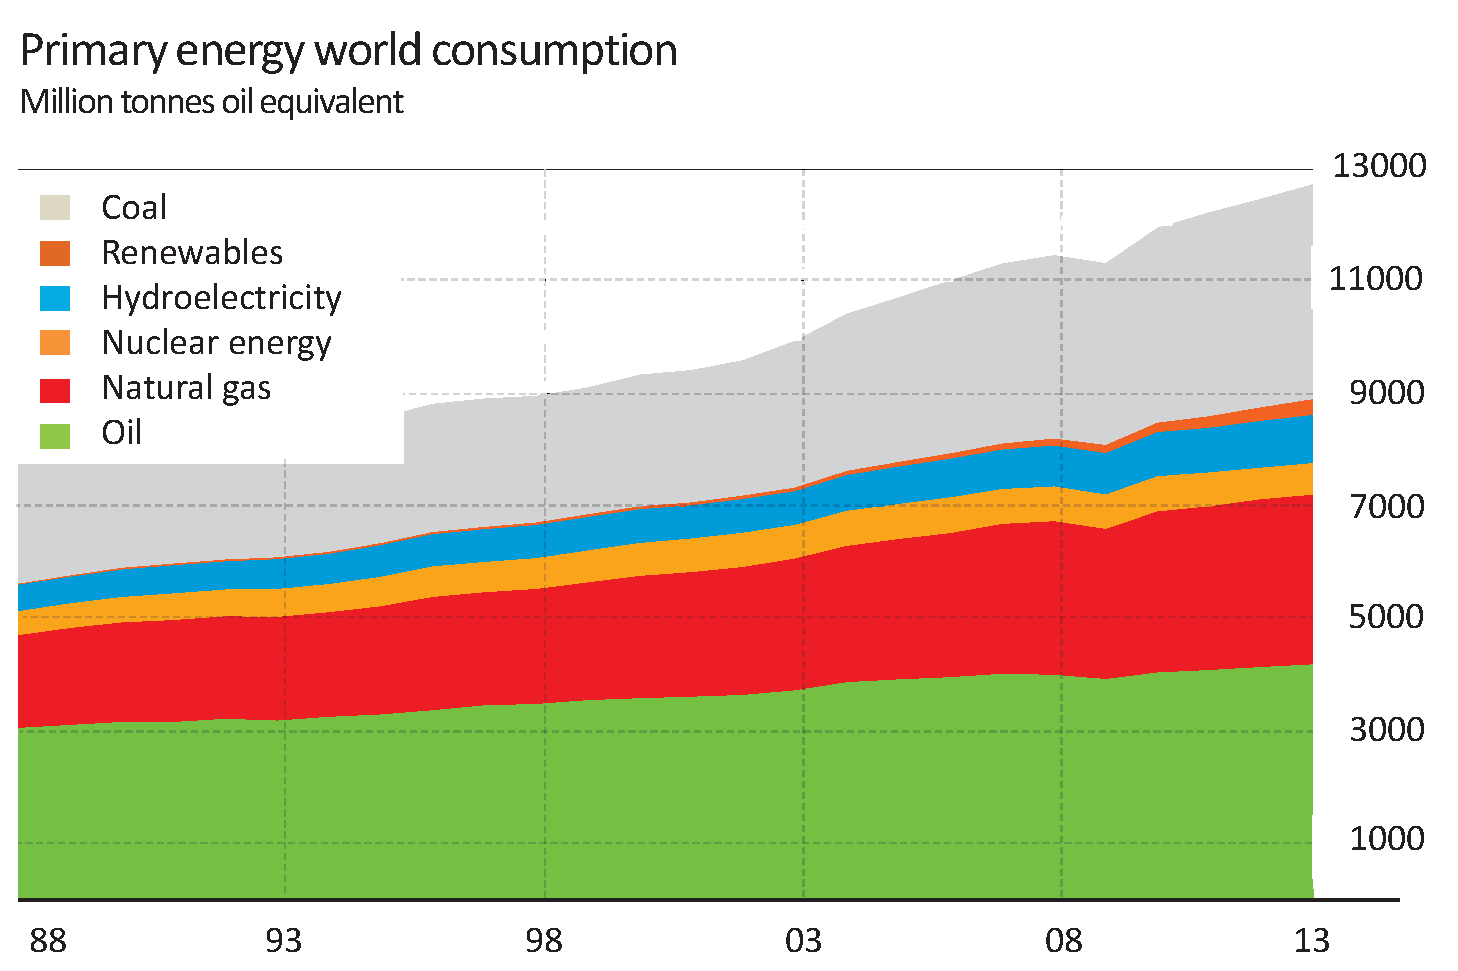
\includegraphics[scale=0.4]{energy.eps}
\caption{Data is from BP statistical review of world energy 2014.}
\label{wpec}
\end{figure}

By the year of 2050, the total world energy consumption will double. Therefore, it is urgent to explore more sustainable and environmentally friendly energy sources. From \textbf{Fig. \ref{wpec}},
one will notice that renewable energy (mainly solar energy, wind power, and geothermal energy) in 2014 accounts for around 2\% of energy consumption globally. It is important to focus on the renewable energy research from a 
long term point of view. The solar energy technologies are one of the hot topic among the renewable energy research considering the point of CO\textsubscript{2} free, reliable energy supply, no cooling water requirement and
operation in silence.

The solar energy technologies are the way to produce electricity from the light of the sun. Sunlight is a portion of the radiation by the sun, like infrared, visible,
and ultraviolet light. The spectrum of the sun is close to the spectrum of black body with a temperature of about 6000 K (\textbf{Fig. \ref{spectrumsun}}). In the field of photovoltaics (PV), solar spectrum is represented
by air mass (AM) which defines the direct optical path length through the Earth's atmosphere. The AM1.5 and AM0 are important: AM1.5 is the air mass at a solar zenith angle of 48.19 degree, and AM0 mean the solar spectrum 
outside of the atmosphere. Generally, the AM1.5 is seen as the reference spectrum in PV field. In \textbf{Fig. \ref{spectrumsun}}, the absorption in the atmosphere is quite stronge by gasses, dust and aerosols, as well as
the scattering of light from air molecules. 

\begin{figure}[H]
\centering
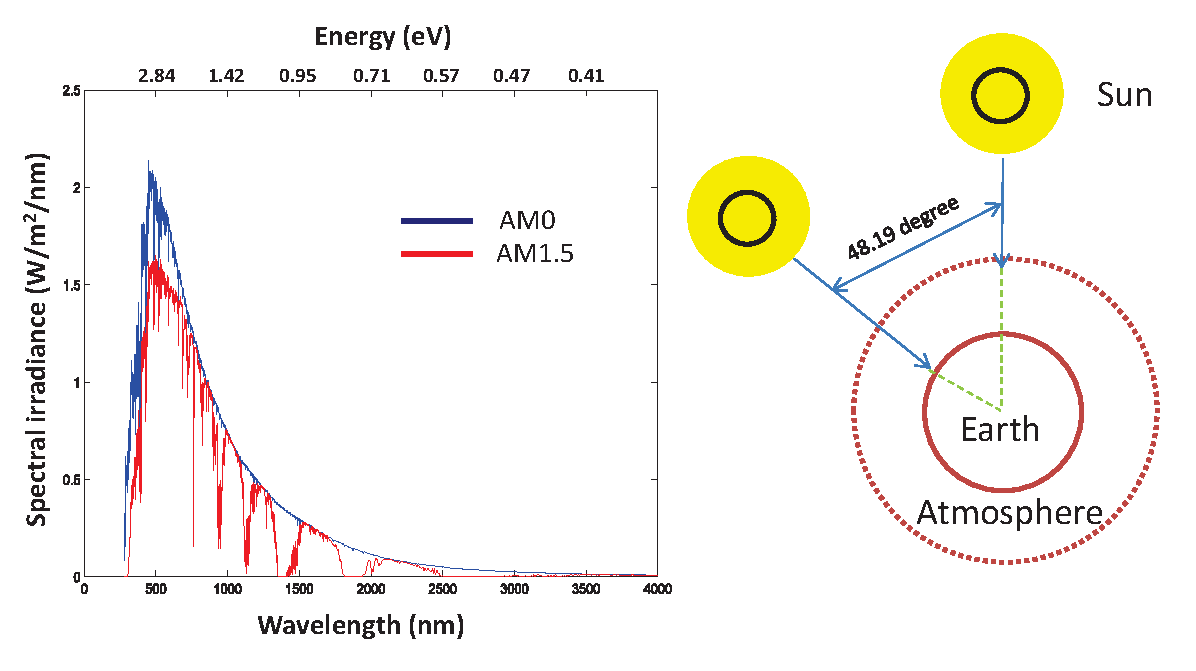
\includegraphics[scale=0.6]{spectrum.eps}
\caption{Solar irradiance spectrum}
\label{spectrumsun}
\end{figure}

There are mainly three kinds of solar energy technologies. The first one is solar thermal,which utilizes the flat sunlight collector plates to harness the energy from sunlight to heat water for use in industries, homes, and pools.
Therefore, the solar thermal collectors do not convert sunlight to electricity directly, but transfer the energy to heat up the water instead. The advangtage is the conversion efficiency is relatively higher. The second one is 
solar chemical, which takes advantage of solar energy by absorbing sunlight in a chemical reaction. However, the conversion efficiency is quite low. The last one is solar photovoltaics (solar cell), which is the way
to utilize solar panels to convert sunlight into electricity. The installation is easier, occupy less space and less maintenance compared with solar thermal. The conversion efficiency is higher than solar chemical. However, 
all the three solar energy technologies are environmentally friendly.


\section{Solar cells}
In the worldwide, the conversion efficiency in all different types of solar cell is improved remarkably. From \textbf{Fig. \ref{nrel}}, one can notice that the highest efficiency for multijunction cells, crystalline silion cells,
thin-film technologies and new emerging cells are around 44.7\%, 27.6\%, 23.3\% and 19.3\%(??by Yang Yang not this figure so far??), respectively. Therefore, the solar cell is a very important and promising way to produce the
renewable energy.

\begin{sidewaysfigure}
\centering
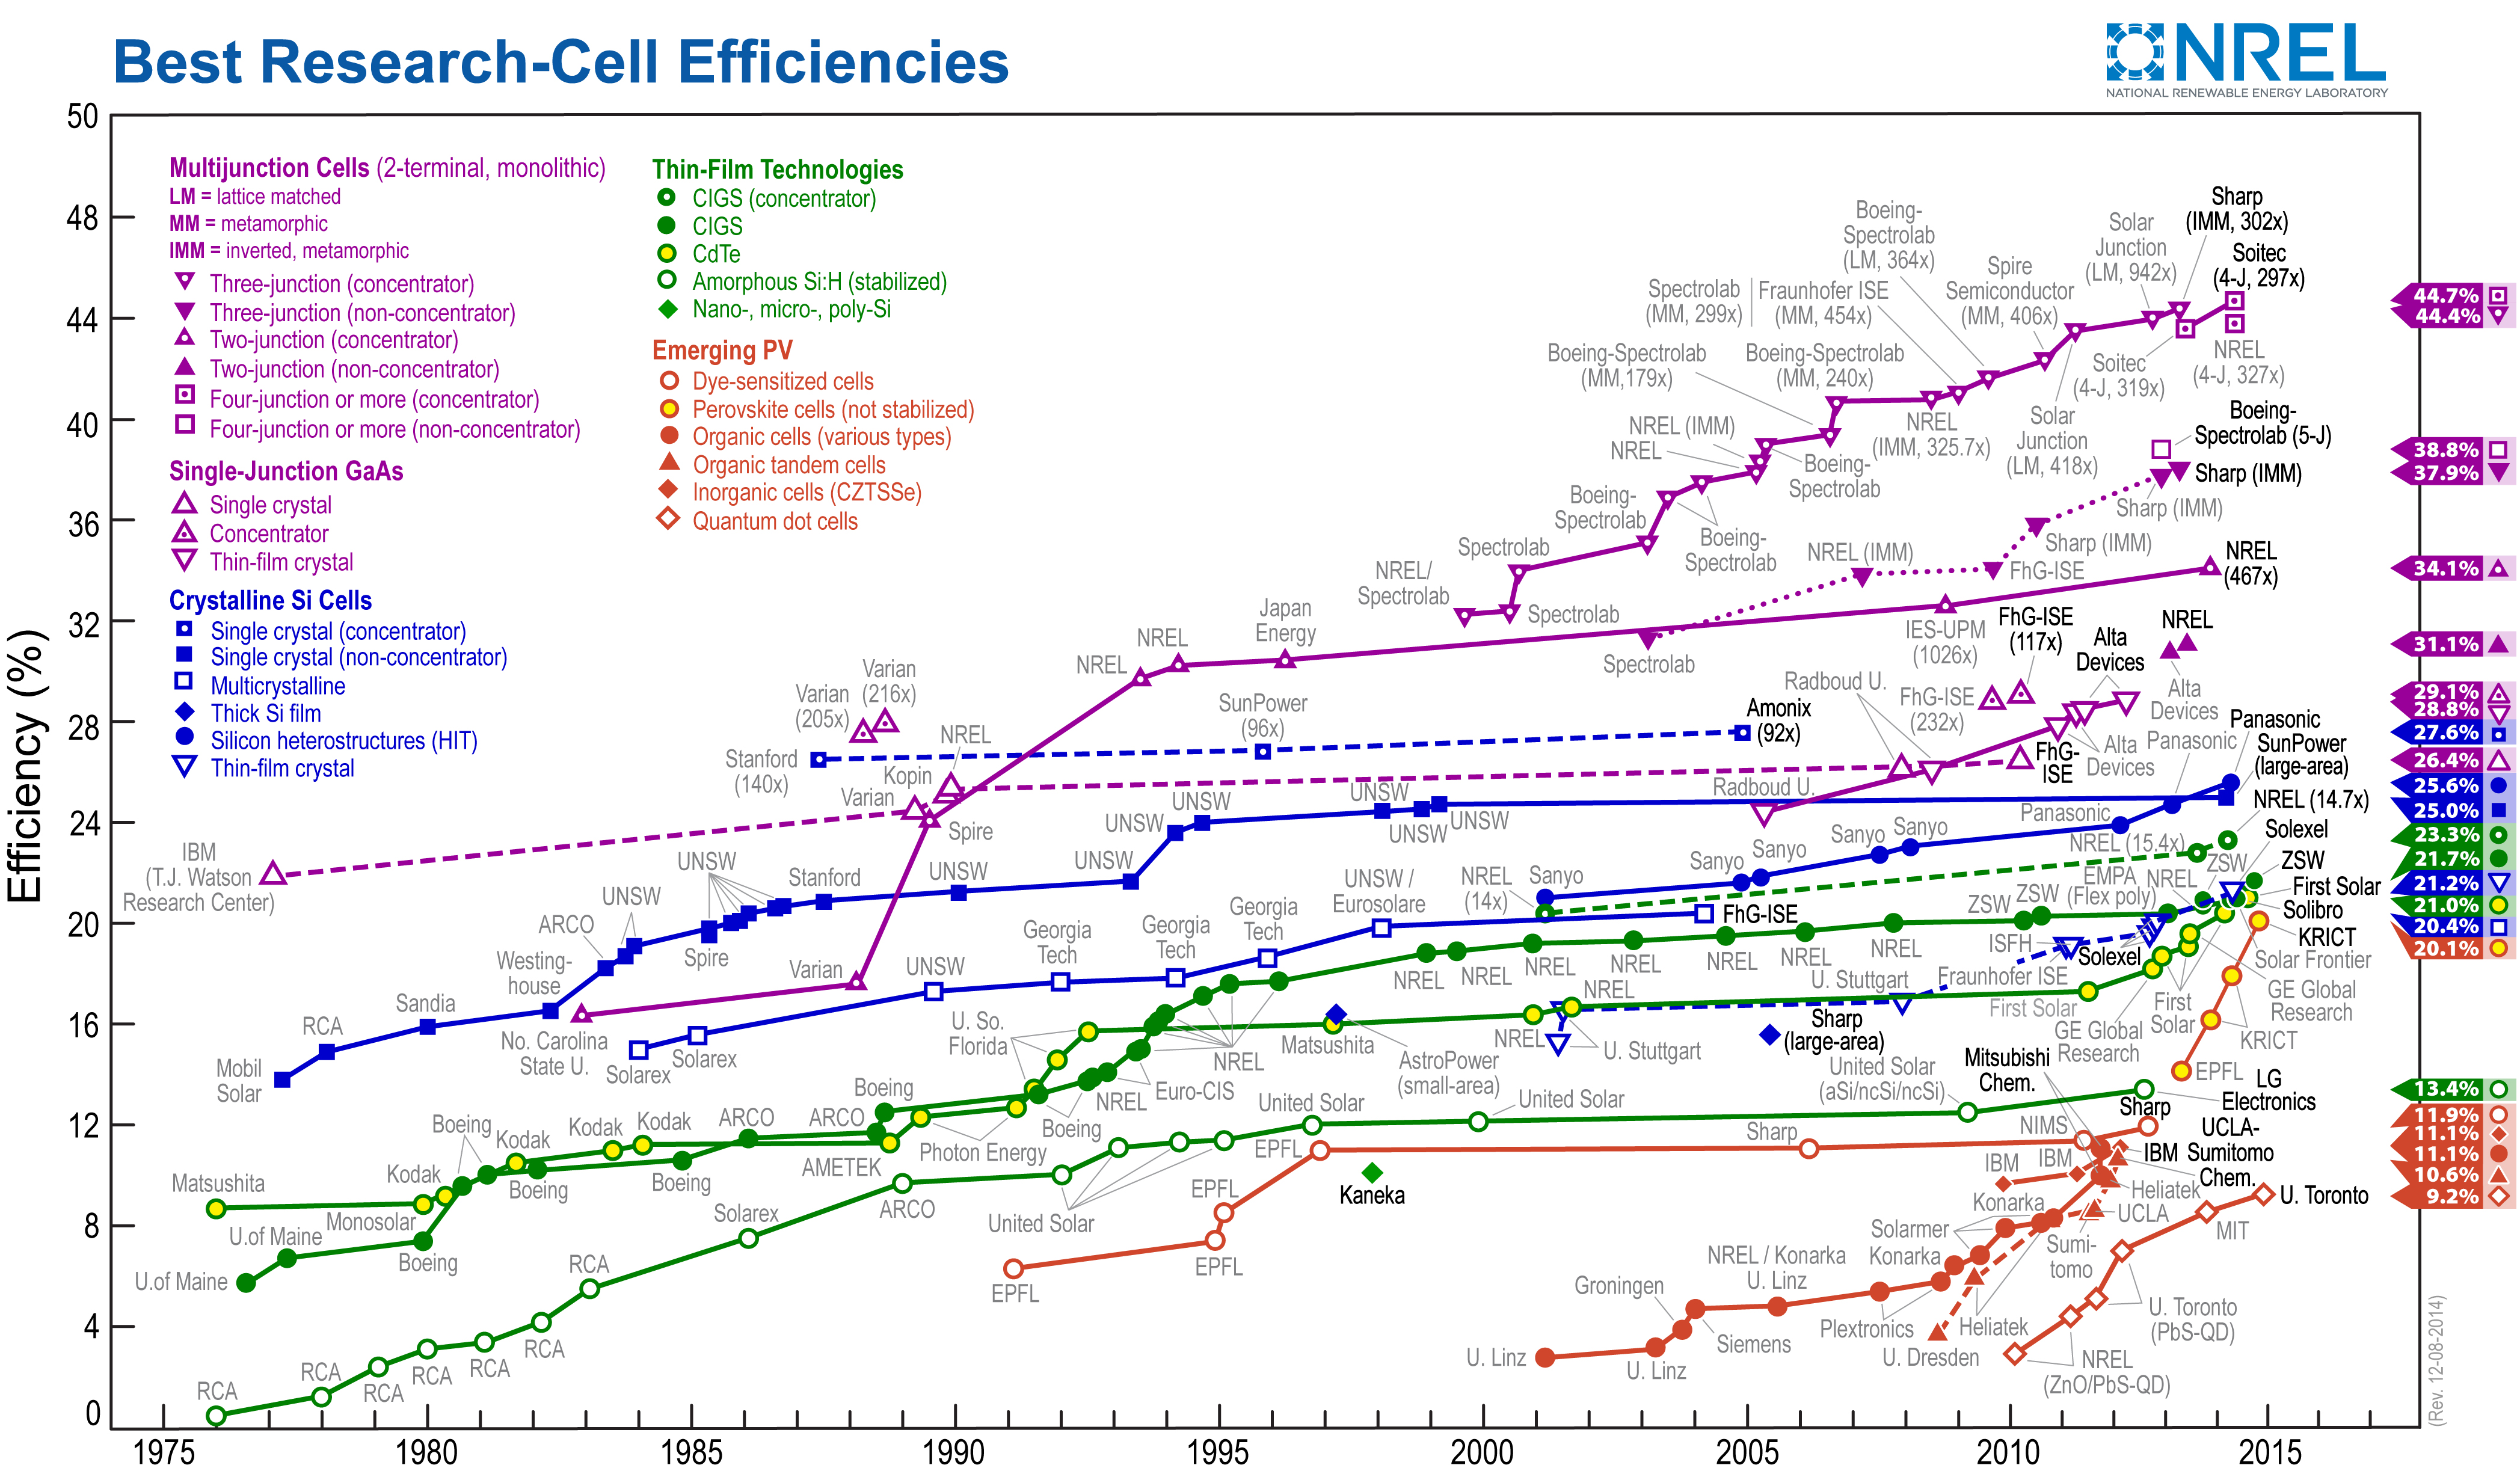
\includegraphics[scale=0.7]{efficiency_chart.jpg}
\caption{Best research-cell efficiencies. Figure is from National Renewable Energy Laboratory (NREL), Golden, Colorado.}
\label{nrel}
\end{sidewaysfigure}

Multijunction cells are the cells which contain multi \textit{p}-\textit{n} junctions (or subcells) which have different band gap for each \textit{p}-\textit{n} junction.
Therefore, different wavelengths of light from the Sun are absorbed for each of junction. For example, wider band gap junction is at the front of the cell, which can absorb the photons with high energy; the junction with 
low band gap can absorb the photos with lower energy. Therefore, the conversion efficiency is higher than singe \textit{p}-\textit{n} junction, for example, the maximum conversion efficiency is 44.7\% by Soitec using 
four-junction or more in \textbf{Fig. \ref{nrel}}. Crystalline silicon cells are the most widely utilized in the photovoltaic industries, which built the solar cells using crystalline silicon (c-Si). It has two types in
the crystalline silicon photovoltaics: mono-crystalline silicon and multi-crystalline silicon. The crystalline silicon cells have high efficiency, for example, the maximum conversion efficiency is 27.6\% with concentrator 
by Amonix and maxium 25.6\% without concentrator by Panasonic in  the \textbf{Fig. \ref{nrel}}. Thin-Film solar cells are the cells which are made by depositing one or several thin layers, which allows the cells to be rather 
flexible and resulting in lower weight. The maximum conversion efficiency is lower than crystalline silicon today, which has the maximum conversion efficiency 23.3\% using CIGS with concentrator by NREL and 21.7\% without 
concentrator by the center for solar energy and hydrogen research (ZSW) in Stuttgart in \textbf{Fig. \ref{nrel}}. The Emerging PV in \textbf{Fig. \ref{nrel}} represents the newest ways to create electricity from
sunlight and potentially with higher conversion efficiency, such as perovskite cells, for which the maximum conversion efficiency is 19.3\% by the group Yang Yang at the University of California, Los Angeles. 
(update the above figure until May, 2014) Perovskite cells jump into the world of solar cells only in 2009, and the conversion efficiency is improved remarkable within 5 years. Certainly, the search and optimisation 
of alternatively solar cell materials is still an ongoing and active area today.


\subsection{Single-junction solar cells}
The \textit{p}--\textit{n} junction is the fundamental building block of solar cells. The single \textit{p}-\textit{n} homojunction will be explored in this section.

We start from the seperate \textit{n}-type material and \textit{p}-type material at room temperature (assume that all the donor (acceptor) atoms are positively (negatively) ionized at room temperature). In \textbf{Fig. \ref{dopedmaterials}}, the left one shows the \textit{n}-type and \textit{p}-type materials. The \textit{n}-type
material has many free negatively charged electrons which can move freely in the material, and there are numbers of positively charged immobile donor ions as well. Similarily, the \textit{p}-type material has many free positively
charged holes which can move freely in the material, and there are numbers of negatively charged immobile acceptor ions as well. However, the material is still neutral in both \textit{n}-type and \textit{p}-type.
On the right in \textbf{Fig. \ref{dopedmaterials}}, the corresponding Fermi levels are shown. The Fermi level (E\textsubscript{nf}) is closer to conduction band minimum for \textit{n}-type material due to the many free 
negatively charged electrons. Conversely, the Fermi level of \textit{p}-type material (E\textsubscript{pf}) is closer to the valence band maximum to the free positively charged holes.

\begin{figure}[H]
    \begin{center}
           % 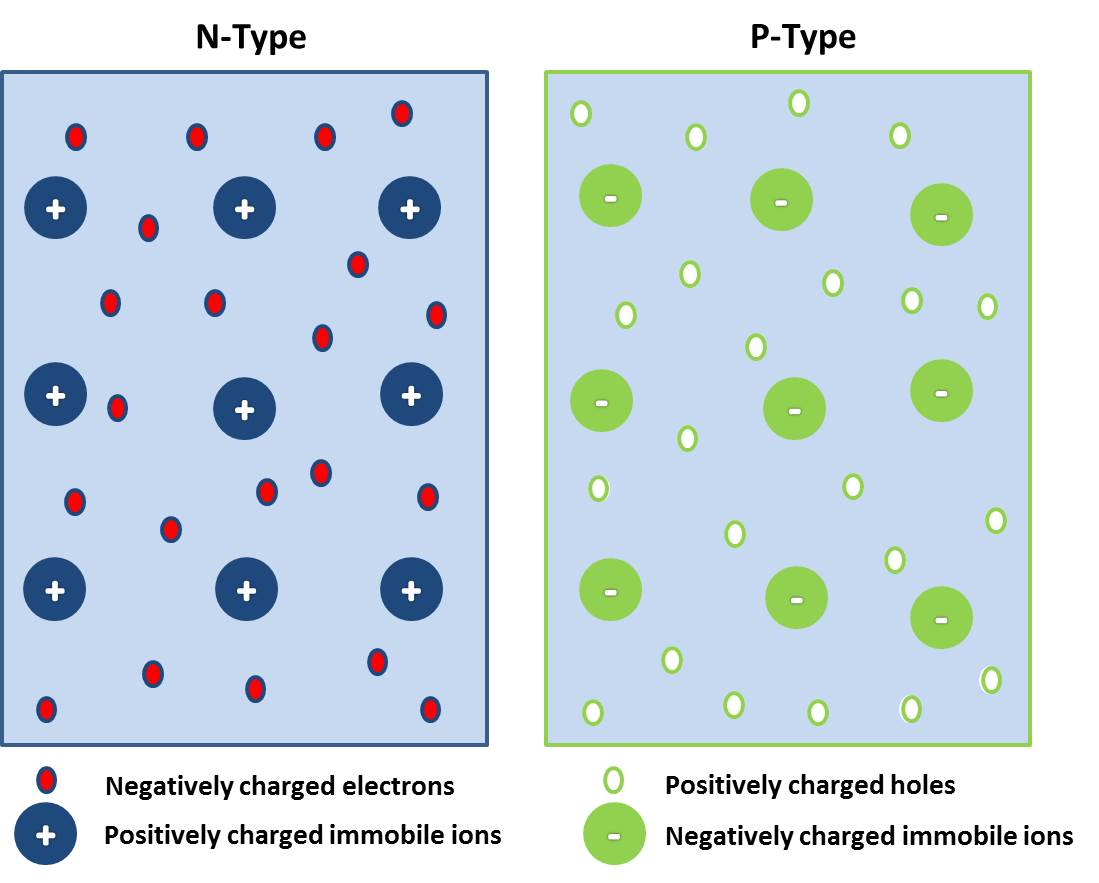
\includegraphics[width=0.4\textwidth,clip]{sepratepn.jpg}
           % 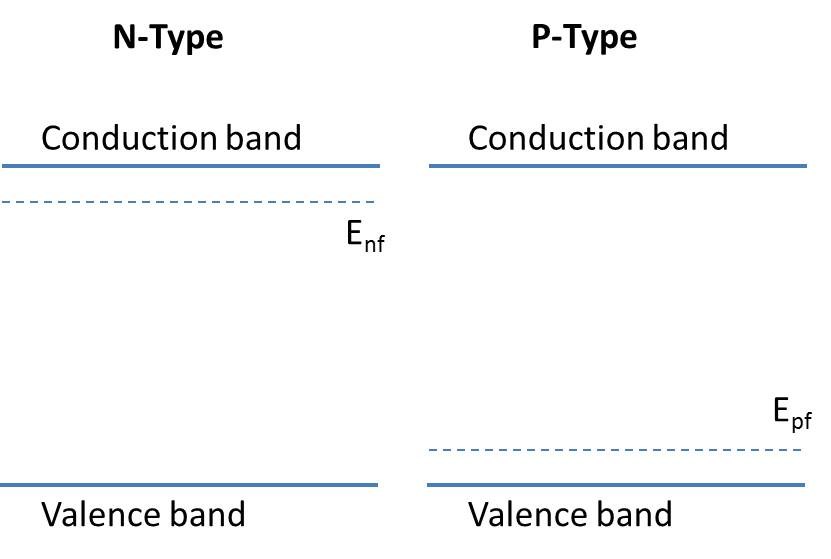
\includegraphics[width=0.4\textwidth,clip]{sepratepn1.jpg}
            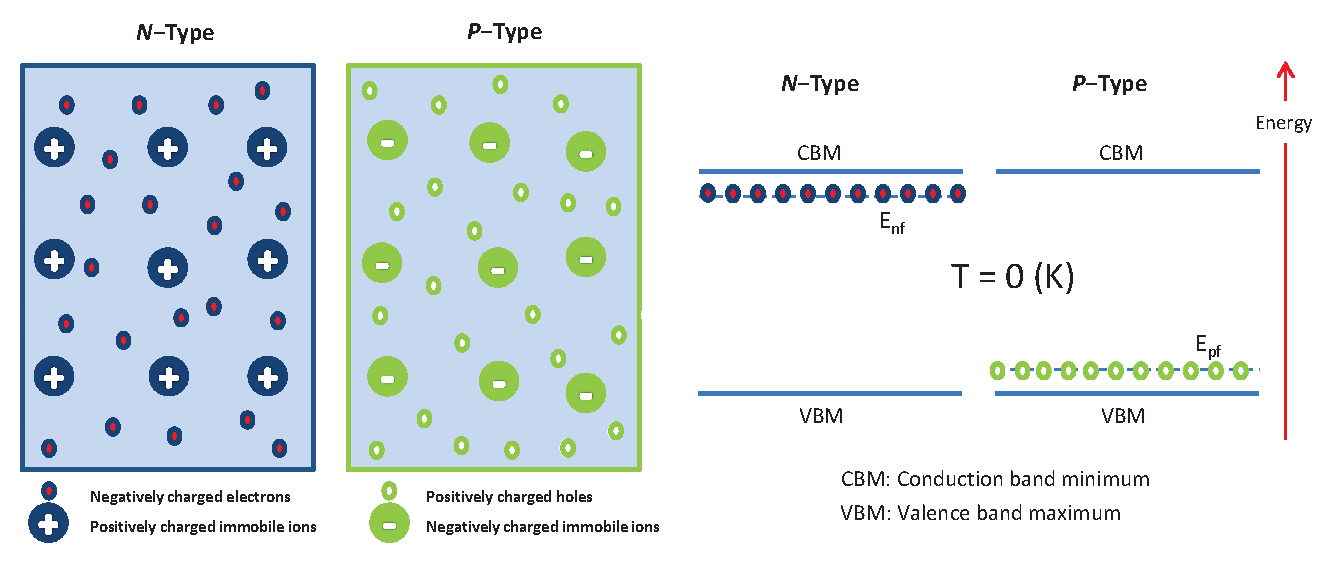
\includegraphics[width=0.8\textwidth,clip]{sepratepn.eps}
     \end{center}
    \caption{Left: Doped (\textit{n}-type and \textit{p}-type) materials in dark at room temperature. Right: Energy band diagram of seperated \textit{p}-\textit{n} homojunction in dark at room temperature for two-level model. Assume that all the donor (acceptor) atoms are 
    positively (negatively) ionized.}      
    \label{dopedmaterials}
\end{figure}

If the \textit{n}-type and \textit{p}-type materials are joined, the free electrons (holes) in \textit{n}-type (\textit{p}-type) material will diffuse into \textit{p}-type (\textit{n}-type) material due to the
lower concentrations of electrons (holes) (\textbf{Fig. \ref{pnjunction}}). In the region which is near the interface between \textit{n}-type and \textit{p}-type materials, the ionized donor and acceptor ions create a
"build in" electric field which points from the \textit{n}-type material to the \textit{p}-type material. This can cause the drift of carriers in the opposite direction. The "build-in" electric field will force the electrons (holes) back into the \textit{n}--type (\textit{p}--type). At certain point, 
the whole material will reach a stable equilibrium due to the achived balance between diffusion and drift. Formation of the "build-in" electric field is rather important for the solar cells, even though there is no currect in 
the material so far. In the following text, the region which forms the "build-in" electric field is also called space charge region (SCR). The different Fermi levels for \textit{n}-type and \textit{p}-type materials are
equal at the stable equilibrium. Therefore, the energy bands bend over and create a potential barrier near the junction (Right in \textbf{Fig. \ref{pnjunction}}). Finally, there is a internal potential V\textsubscript{bi}
in the junction, which will block the diffusion.

\begin{figure}[H]
    \begin{center}
           % 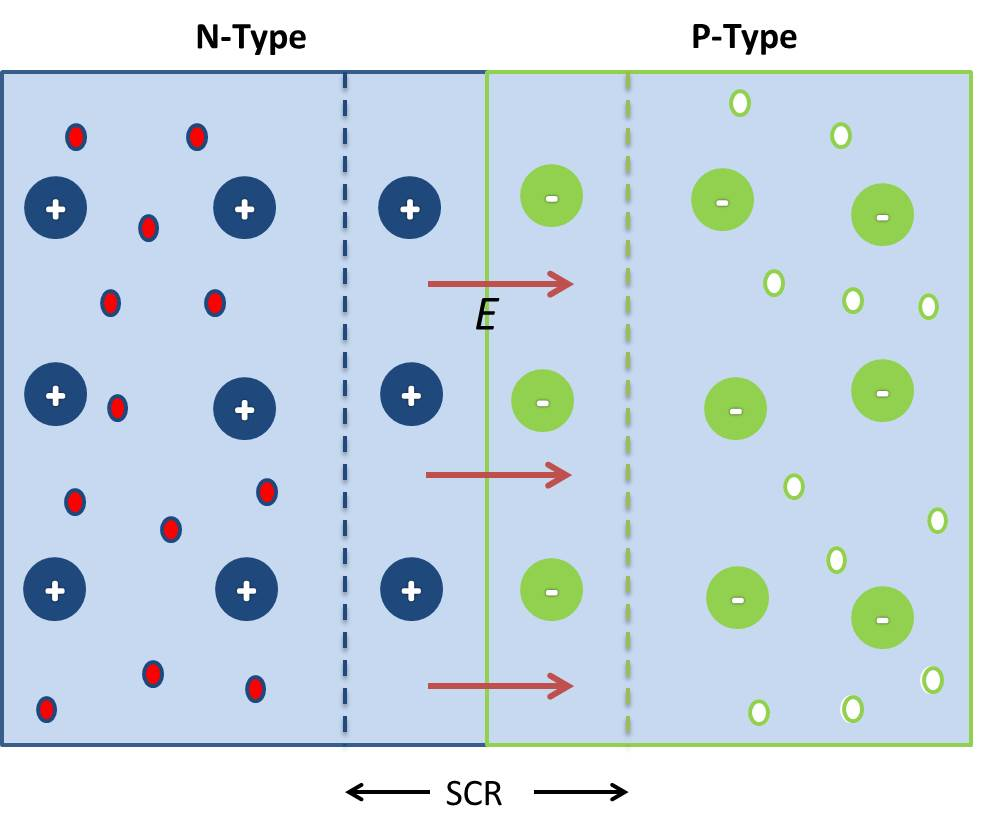
\includegraphics[width=0.4\textwidth,clip]{pnjunction.jpg}
           % 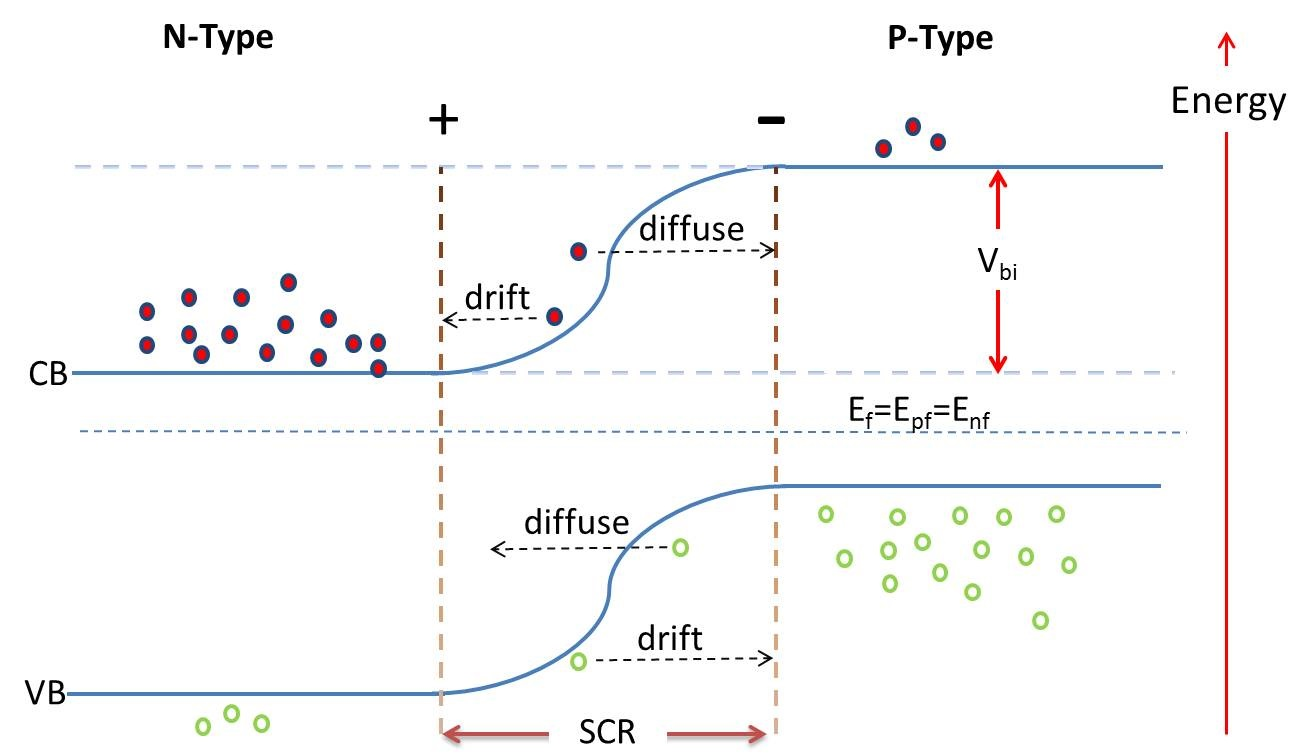
\includegraphics[width=0.5\textwidth,clip]{pnjunction1.jpg}
            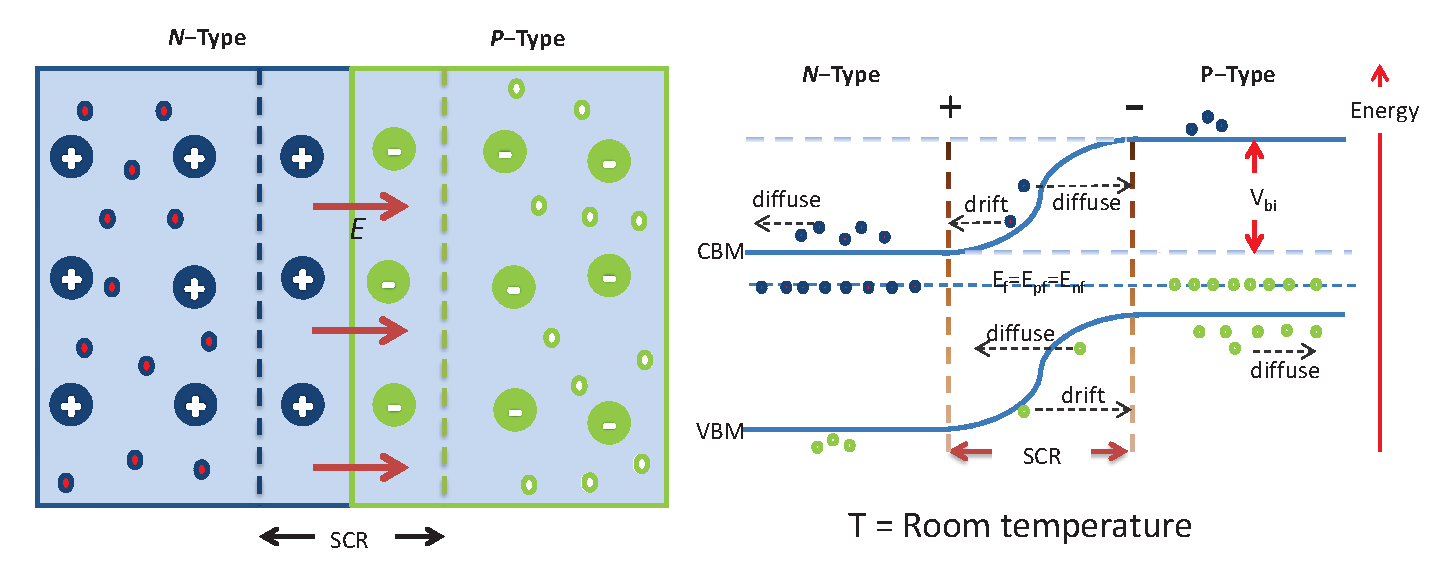
\includegraphics[width=0.7\textwidth]{pnjunction.eps}
     \end{center}
    \caption{Left: The \textit{p}-\textit{n} homojunction in dark at room temperature. Right: Energy band diagram of a \textit{p}-\textit{n} homejunction at the equilibrium in dark at room temperature for two-level model. }      
    \label{pnjunction}
\end{figure}

The \textit{p}-\textit{n} junction cell with and without the illumination is discussed in \textbf{Fig. \ref{illu}} and \textbf{Fig. \ref{illu1}}. If there was a wire with certain resistance connecting 
the \textit{n}-type and \textit{p}-type, there is no current in the wire under the condition of dark (no illumination). However, if the light shines on the cell or component, a current will be generated from the \textit{p}-type
to the \textit{n}-type side (conventional current). Because the electrons from valence bands (VBs) goes to conduction bands (CBs), which can generate pairs of electron-hole. At the same time, the recombination of paired electron-hole ocurrs. The rate of generation 
is faster that of recombination, therefore, net generation occurs. Apparently, there are three regions in the whole junction cell where the electrons goes from VBs to CBs, the \textit{n}-type region, the \textit{p}-\textit{n}
junction, and the \textit{p}-type region. In the either \textit{n}-type or \textit{p}-type region (especially, region which is far away SCR), the electron–hole pairs can not remain long time,  it is most probable that electrons
will jump down from CBs to VBs again. However, the electron-hole pairs will be seperated in the \textit{p}-\textit{n} junction region due to the "build-in" electric field, therefore, the current will be generated. Actually, the electron-hole pairs in the either n-type and p-type 
(especially, for them which are near SCR) also have the chance to diffuse into the SCR, it will contribute the generation of current or reduce the current.

\begin{figure}[H]
\centering
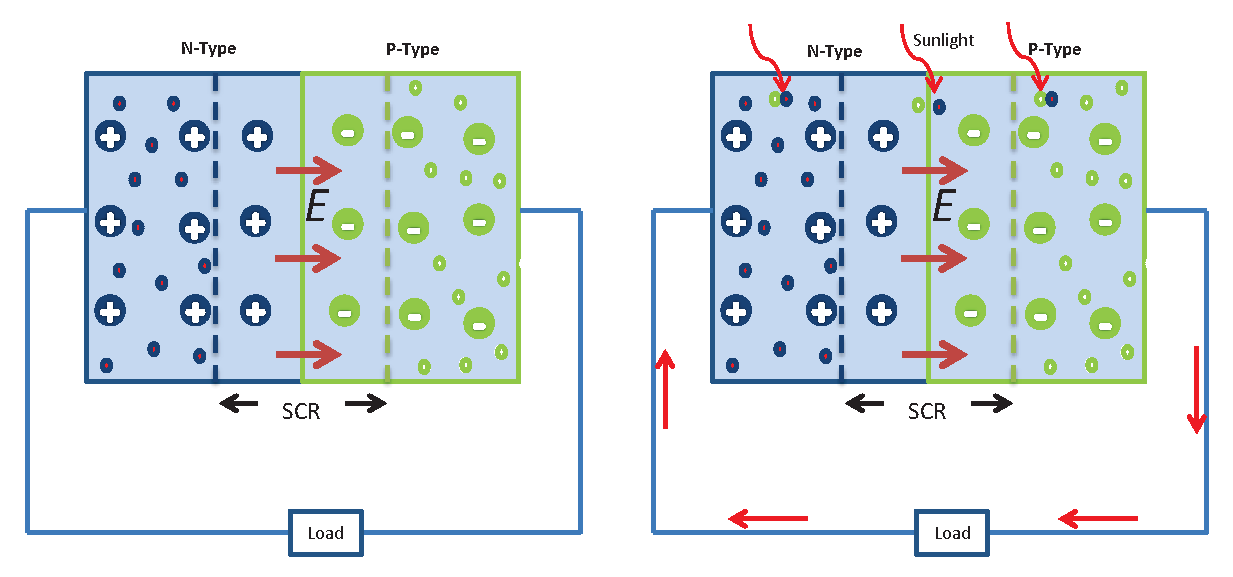
\includegraphics[scale=0.5]{illumination.eps}
\caption{The \textit{p}-\textit{n} homejunction under illumination with load at room temperature for two-level model.}
\label{illu}
\end{figure}

In \textbf{Fig. \ref{illu1}}, the SCR becomes more "smooth" due to the extra load, such as lightbulb, which is equivalent to apply external potential. The stablized Fermi level at the stable equilibrium splits under illumination.
The chemical potential $\bigtriangledown \mu = E_{nf} - E_{vf}$ is created, which is considered as the electron charge times the voltage across the device. The generation and recombination by impuriteis are not analyzed in here.

\begin{figure}[H]
\centering
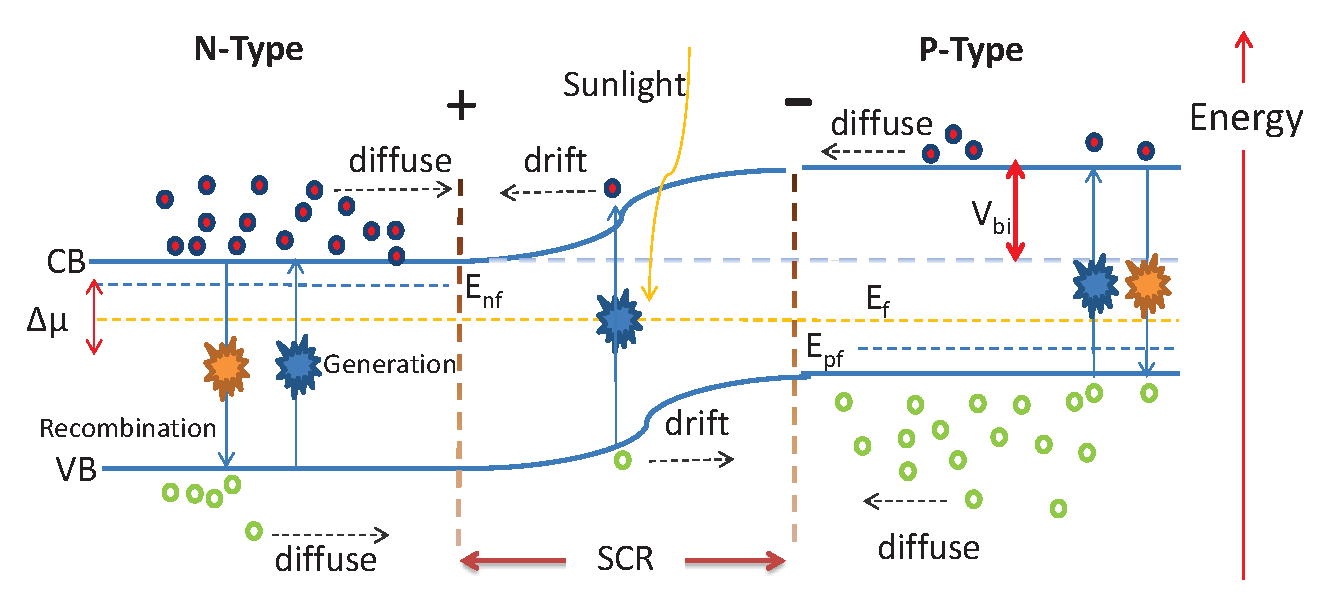
\includegraphics[scale=0.5]{illumination1.eps}
\caption{Energy band diagram of a \textit{p}-\textit{n} homojunction under illumination with load.}
\label{illu1}
\end{figure}


The I-V characteristics is defined in \textbf{Fig. \ref{ivcharac}} with some important parameters of the solar cells. The $V_{oc}$ and $I_{sc}$ are the open circuit voltage and short circuit current, respectively. 
They are the maximum voltage and maximum current from the solar cells. The $V_{mp}$ and $I_{mp}$ are the voltage and current which will yield the maximum power. The maximum power generated by the solar cells is $P_{out}=V_{mp} \times I_{mp}$, that is the rectangle bounded by the dashed lines in the 
\textbf{Fig. \ref{ivcharac}}. 

\begin{figure}[H]
\centering
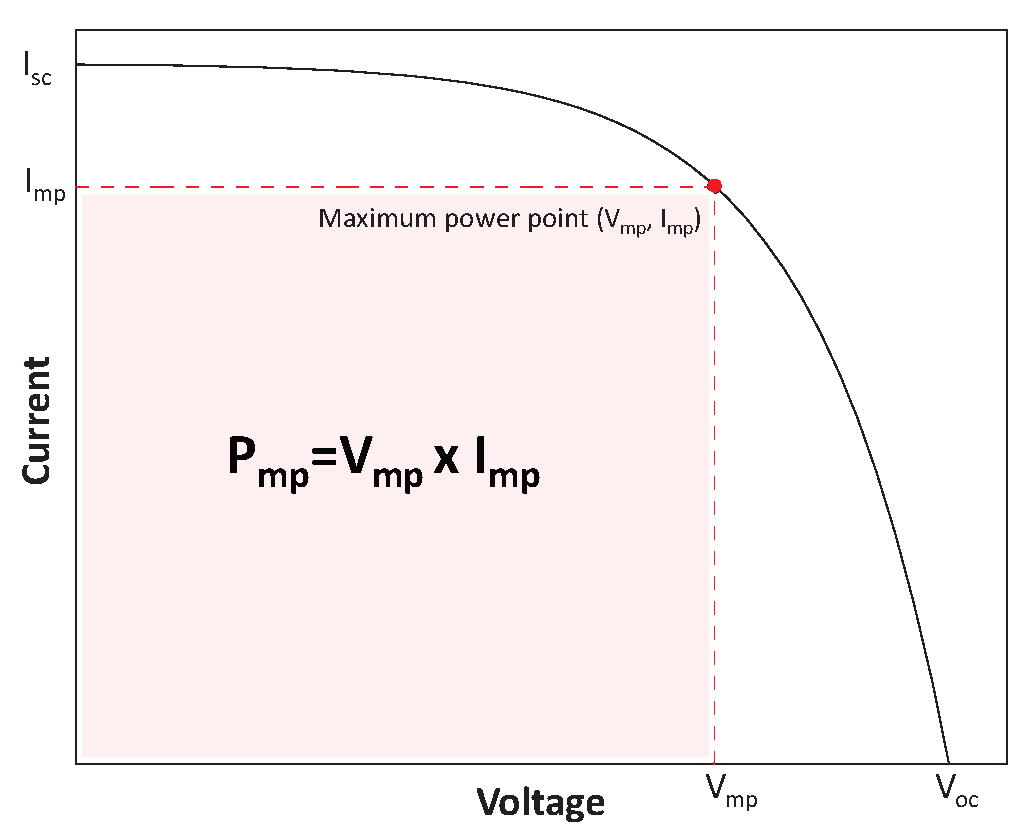
\includegraphics[scale=0.5]{IV.eps}
\caption{I-V characteristics}
\label{ivcharac}
\end{figure}


The fill factor (FF) and the power conversion efficiency ($\eta$) are often represented the solar cell performance:

\begin{equation}
FF = \frac{P_{out}}{V_{oc} \cdot I_{sc}} = \frac{V_{mp} \cdot I_{mp}}{V_{oc} \cdot I_{sc}}
\end{equation}

\begin{equation}
\eta = \frac{P_{out}}{P_{in}} = \frac{FF \cdot V_{oc} \cdot I_{sc}}{P_{in}}.
\end{equation}

Here, $P_{in}$ is the incident photon power per second. The conversion efficiency of the solar cells is proportional to FF, $V_{oc}$, and $I_{sc}$. There are several aspects which will affect
the conversion efficiency. $V_{oc}$ is directly proportional to the band gap of the material, $I_{sc}$ is proportional to the number of absorbed photons. When the band gap is decreased, the more of the spectrum is absorbed. However, 
the $V_{oc}$ will be reduced in this case, more importantly, the excess energy of photons is lost due to the thermalization in the cells. When the band gap is increased, transparency losses from the photons with energy lower than band 
gap. There is more detailed analysis of conversion efficiency in the Ref[?? Principles of solar energy conversion].


\section{Solar cell materials}

In 1839,  the French physicist A. E. Becquerel revealed the photovoltaic effect for the first time. Charles Fritts built the first solid state photovoltaic (PV) cell using semiconductor selenium in 1883. It is not until 1941 that
the first silicon-based solar cell was demonstrated. Today, there are many different types of solar cell materials. The reason why the best solar cell material is not realized yet is that it is expected to be not only high efficiency but 
also environmentally friendly and low cost. It requires not only that the growth and manufacturing prcess of solar cell materials shall be cheapter, but also that the devices shall have longer application life, moreover the raw material
should be abundant and non-toxic as well. In this section, four main solar cell materials are discussed briefly: silicon (Si), gallium arsenide (GaAs), cadmium telluride (CdTe), copper indium gallium diselenide (Cu(In,
Ga)Se\textsubscript{2}).

Potential solar cell materials need to fullfil several properties, such as large absorption coefficient and a band gap energy Eg between 0.7 to 2.0 eV. Under these conditions, there are quite many materials satisfying the 
requirements. However, some other properties are needed to be considered as well, such as cost and enviromental safety. Thereby, only part of them are suitable to produce in reality. In \textbf{Fig. \ref{lscm}}, several solar cell
materials are illustrated. 

\begin{figure}[H]
\centering
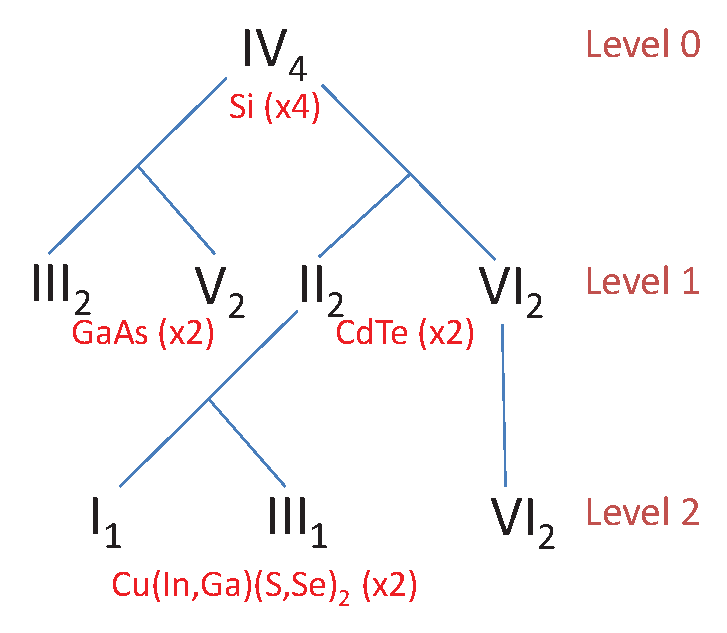
\includegraphics[scale=0.5]{tree.eps} 
\caption{Tree of tetragonal bonded semiconductor, the roman numerals mean the group numbers in the chemical element periodic table, and the subscript implies the number of elements.}
\label{lscm}
\end{figure}

In \textbf{Fig. \ref{lscm}}, the formation of tetragonal semiconductors is considered as a series of cation mutations where the total number valence electrons is the same and keep the charge neutral. For example, group number
IV element silicon (level 0) with four 4\textsuperscript{+} ions is equivlant to two 3\textsuperscript{+} ions and two 5\textsuperscript{+} ions, such as GaAs (level 1). It is also equivlant to two 2\textsuperscript{+} ions
and two 6\textsuperscript{+} ions, such as CdTe (level 1). The Cu(In,Ga)(S,Se)\textsubscript{2} can be generated applying the same process on II element on the level 1. This method was suggested by Goodman and Pamplin. 



\subsection{Crystalline silicon solar cells}
The solar cell based on silicon dominates the solar power world today, which accounts for more than 90\% of the total PV market.
This kind of solar cell takes advantage of different forms of silicon, that is, monocrystalline silicon and polycrystalline silicon. 
The success of Si is due to a number of reasons. Over 90\% is composed of silicate minerals in the crust of earth, which also yields huge available amounts of Si. Moreover, it has higher conversion efficiency, and it is also proved that 
it has excellent stability and reliability under the outdoor condition. However, Si also have drawbacks. It has an indirect band gap and hence it has a lower optical absorption coefficient. In order to absorb the incident sunlight fully, 
it requires to thicker Si (around \SI{40} {\micro\meter}) to absorb the sunlight. Crystalline Silicon have to be high quality and defect free in order to avoid losting the carriers before collection. Last but not least, it is costy to purify the Si from silicate minerals, which
really limits the cost reduction potential of wafer-based silcion technology. 

However, the solar cells based crystalline silicon technology is still leading the market of solar cell since many companies are trying to lower the cost of the whole process.



\subsection{Gallium arsenide}
Gallium arsenide (GaAs) has a zinc blende crystal structure with a direct band gap around 1.5 eV at room temperature. Some electronic properties of GaAs are superior to Si, such as higher electron 
mobility, higher saturated electron velocity, absorb sunlight more efficiently due to the direct band gap. The optimum band gap for the single junction solar cell is suggested around 1.3 eV by theoretical calculation 
from Henry (1980) who modified the originial Shockley-Queisser limit. Therefore one of the most applications of GaAs is solar cells. GaAs has been extensively researched since the 1950s, and the first GaAs solar cells were established in
1970 by the Zhores Alferov's team. Today, the conversion efficiency for single function solar cell based on GaAs is around 28.8\%. However, it is more difficult to grow and the solar cell component has higher price in comparison with Si.
Many researches are focusing on how to reduce the price, and the main application solar cell based on GaAs is in the space application. At last, the arsenic toxicity should be considered as well. 

The conversion efficiency for four-junction GaInP/GaAs//GaInAsP/GaInAs concentrator solar cells is reached 44.7\% by Soitec on March 2014.

\subsection{Thin film materials}

Thin film solar cells have several thin films with the total thickness less than \SI{10} {\micro\meter}. The cost can potentially be lower since the less materials are utilized to make thin film solar cells. The development of thin film
solar cell was started since 1970s. Currently, the conversion efficiency for the single junction already surpassed 20\%, even though it is still not as high as the solar cells based on crystalline silicon. Three different thin film
materials are discussed in this section: amorphous silicon (a-Si), cadmium telluride (CdTe), and copper indium gallium diselenide (CIGS).

Amorphous silcion solar cells are the first thin film solar cell material which reach the large-scale production. It has higher absorption coefficient than crystalline silicion, therefore, the thickness can be less than \SI{1} {\micro\meter}. The 
main disadvantages a-Si solar cells is the lower efficiency, the actual conversion efficiency for the commericial single junction solar cells based on a-Si is between 4\% to 8\%. This limits the development of a-Si thin film solar cells.
A-Si solar cells are suited to the situation which requires low cost over high efficiency. 

CdTe was first reported in the 1960s. However, it is not developed rapidly until in the early 1990s. CdTe has a number of advantages as an absorber. It has higher absorption coefficient. The band gap is around 1.45 eV, which 
is very near the optimum value for single-junction solar cells. Moreover, the manufacturing process is easier to control, which results in the cost of manufacturing is low. Moreover, the commercial modules already reach the efficiency of 16\%.
However, an important question is needed to be considered in order to large-scale CdTe manufacturing: cadmium toxicity and tellurium availability. 

CIGS are direct band gap seciconductors with high optical absorption coefficients. It is seen as the most promising solar cell material for the near future. It is always employed in a heterojunction structure, mainly it is with the thinner
\textit{n}-type CdS layer. The conversion efficiency of CIGS reached up to 20\% in the laboratory cell. The intersting part is that it can be alloyed by the ratio of Ga/(Ga+In), and the band gap can be tuned along with that. The band gap 
is between 1.0 eV to 1.7 eV for this alloy. CIGS does not contain any toxic element.

\section{CuIn\textsubscript{1-\textit{x}}Ga\textsubscript{\textit{x}}Se\textsubscript{2}(CIGS) materials}
CIGS material is a chalcopyrite-type material, which is considered to be one of the most promising thin film solar cell material. The direct band gap is from around 1.0 ev to 1.7 eV by alloying Ga in the CuInSe\textsubscript{2},  and the conversion efficiency in laboratory already surpassed 20\%. 
CuInSe\textsubscript{2} was first synthesized by Hahn in 1953. It was first exploited as an absorber material in a single crystal solar cell in 1974, which is based on CuInSe\textsubscript{2} and CdS. The conversion efficiency is around 
5\%. The first thin film solar cells based on CuInSe\textsubscript{2} and CdS was invented by Kazmerski. During 1980s, Boeing Corporation did much reseach on the thin film polycrystalline CIGS solar cells. 
To date, the highest conversion efficiency in lab situation for the solar cells based on CIGS is between 20\% and 21\% by alloying with Ga.


\subsection{Crystal structure}
The crystal structure of CIGS can be derived from the zinc blende crystal structure of zinc selenide (ZnSe). In the \textbf{Fig. \ref{crystal_cigs}}, the crystal structures of ZnSe and CIGS are presented. 
The elements Zn are replaced by Cu and In or Ga elements in the zinc blende of ZnSe. It requires to double the unit cell in the z-direction. Because the bond strength and lengths between
Cu-Se and In-Se or Ga-Se are different, therefore, the lattice parameter c is not exact 2a normally.

Chalcopyrite CIGS (with x = 0.0 and 1.0) has the space group $D_{2d}^{12}$ ($I\overline{4}2d$; space group no. 122).
The conventional unit cell has four copper atoms on the Wyckoff positions 4a, four indium/gallium atoms on position 4b, and eight selenium atoms on the 8d position. 
The cation positions have all $S_4$ point-group symmetry, and Se have $C_2$ symmetry. 
The Se 8d position is fully defined with the position (x, y, z), and each anion Se-atom has two inequivalent bonds $\delta$X–Se to the cations X = Cu and In/Ga. 
For the alloy of CIGS (in this work, x = 0.5 with 50\% In and 50\% Ga), the structure is chosen so that each Se atom bonds to two Cu atoms, one In and one Ga atom. The space group is $S_{4}^{2}$ ($I\overline{4}$; space 
group no. 82).


\begin{figure}[H]
\centering
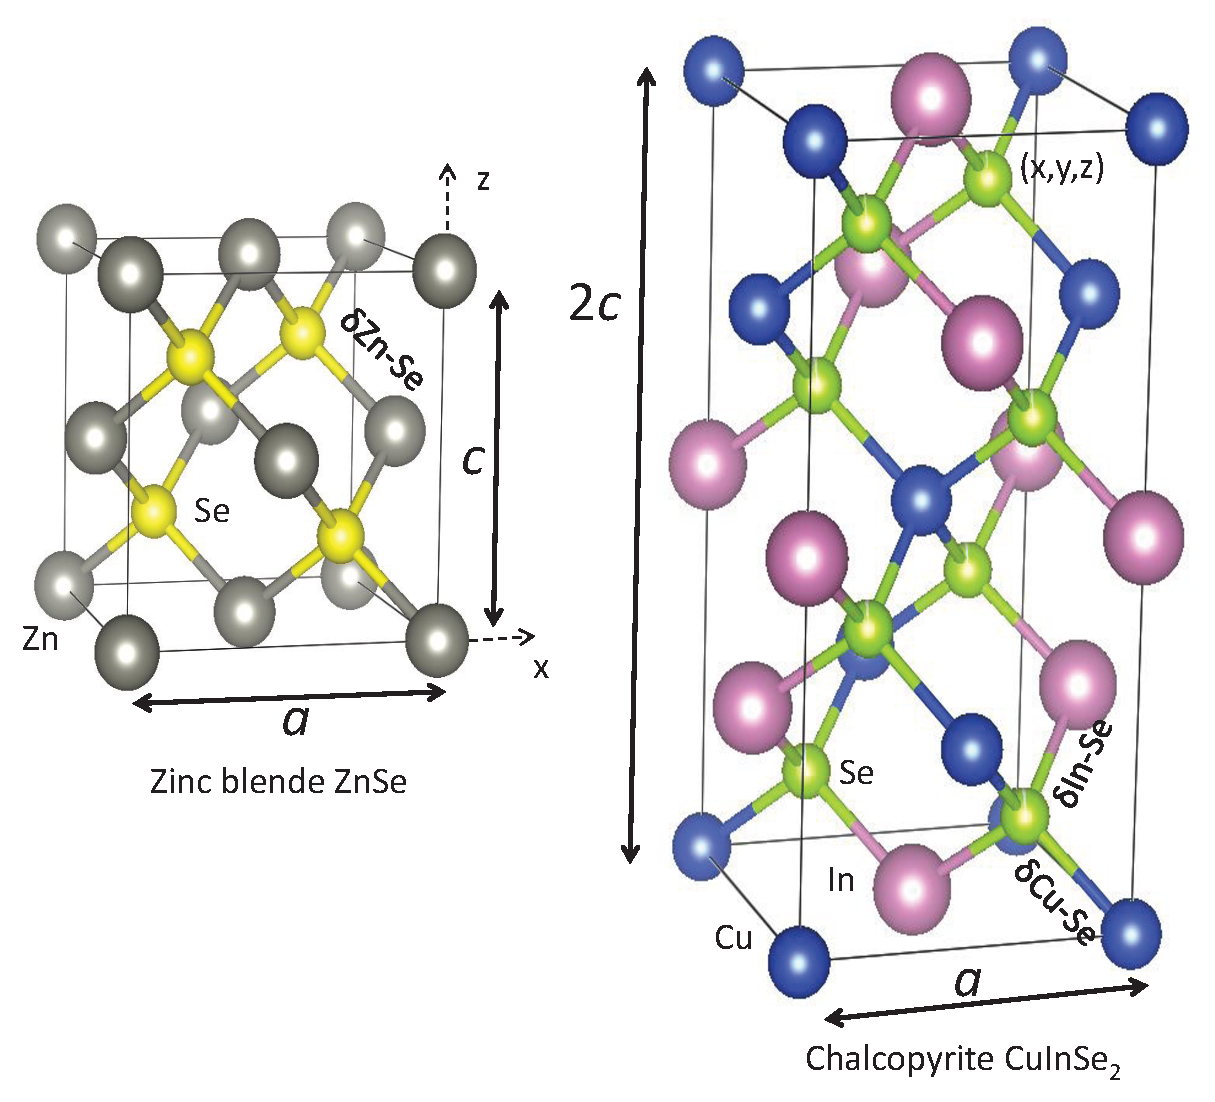
\includegraphics[scale=0.4]{structureciise.eps} 
\caption{}
\label{crystal_cigs}
\end{figure}






\subsection{Optical properties and defects in the CIGS}
CuInSe\textsubscript{2} has a direct band gap around 1.0 eV, and the absorption coefficient is relatively higher than Si due to direct band gap. The quaternary CIGS alloy will be available by alloying Ga element, while the band gap is tuned as well from 
1.0 eV to 1.7 eV. The high absorption coefficient makes the CIGS material possible to be an absorber for the thin film solar cells. The band gap can be approximated by the function of Ga content (x):

\begin{equation}
E_g(x) = 1.0 + 0.564x+0.116x^2
\end{equation}

Alloying the Ga element will decrease the electron affinity of CIGS, which will make the conduction band upward shift, however, the valence band remain the same postion. This also explains the reason why the band gap increases with 
more Ga element in the CIGS materail. An overview properties of CIGS material is described in \textbf{Table. \ref{kth518}} 


\vspace{10cm}

\begin {table}[!htb]
\centering
\begin{tabular}{l l l}  
\toprule
\toprule
%\rowcolor[gray]{0.7}
\multicolumn{3}{c}{\large Properties of CuInSe\textsubscript{2} and CuGaSe\textsubscript{2}} \\  
%\midrule
\cellcolor{blue!25} Properties & \cellcolor{blue!25} CuInSe\textsubscript{2} & \cellcolor{blue!25} CuGaSe\textsubscript{2} \\ 
%\midrule

Space group & $D_{2d}^{12}$(I$-$42d), no. 122 & $D_{2d}^{12}$(I$-$42d), no. 122 \\ 
%\midrule
\rowcolor[gray]{0.9}
Lattice constants (Å) & \textit{a} = \textit{b} = 5.78, \textit{c} = 11.55 & \textit{a} = \textit{b} = 5.61, \textit{c} = 11.00 \\ 
                      & \textit{a} = \textit{b} = 5.78\textsuperscript{d}, \textit{c} = 11.64\textsuperscript{d} & \textit{a} = \textit{b} = 5.61\textsuperscript{e}, \textit{c} = 11.02\textsuperscript{e} \\ 
%\midrule
Wyckoff positions & Cu:4a, In:4b, Se:8d & Cu:4a, Ga:4b, Se:8d \\ 
%\midrule
\rowcolor[gray]{0.9}
Direct band gap (eV) & Eg = 1.04 & Eg = 1.68 \\ 
%\midrule
Effective masses on $\Gamma$ point (m\textsubscript{0}) & Electrons: 0.08& Electrons: 0.14\textsuperscript{b} \\ 
                                      & Holes(heavy): 0.72& Holes(heavy): 1.2\textsuperscript{c} \\ 
                                      & Electrons: 0.08\textsuperscript{a} & Electrons: 0.13\textsuperscript{a}\\
                                     & Holes(heavy): 0.23\textsuperscript{a} & Holes(heavy): 0.32\textsuperscript{a} \\ 
%\midrule
\rowcolor[gray]{0.9}
Main intrinsic defects & \textit{p}-type: V\textsubscript{Se}; In\textsubscript{Cu}&  \textit{n}-type: V\textsubscript{Se}; Ga\textsubscript{Cu}\\
\rowcolor[gray]{0.9} & \textit{p}-type:  V\textsubscript{Cu}; Cu\textsubscript{In} & \textit{p}-type: V\textsubscript{Cu}; Cu\textsubscript{Ga}  \\  
%\midrule
Crystal field splitting $\Delta_{cf}$ (eV) [300K] & 0.006, 0.007\textsuperscript{a} & $-$0.09, $-$0.104\textsuperscript{a} \\ 
%\midrule
\rowcolor[gray]{0.9}
Spin-orbit splitting $\Delta_{so}$ (eV) [77K] & 0.23, 0.193\textsuperscript{a} & 0.231, 0.210\textsuperscript{a} \\ 
%\midrule
Dielectric constants $\varepsilon(0)$ & 13.6\textsuperscript{d},15.7\textsuperscript{d} & 11.0\textsuperscript{d}, 8.5\textsuperscript{d}\\
%\midrule
\rowcolor[gray]{0.9}
Melting temperature (K)& 1259 & 1310 $-$ 1340\\
%\midrule
Thermal expansion coefficients [300K] 1/K & a axis: 11.23$\times$10\textsuperscript{$-$6}& a axis: 13.1$\times$10\textsuperscript{$-$6}(landolt)\\
& c axis: 7.90$\times$10\textsuperscript{$-$6}&c axis: 5.2$\times$10\textsuperscript{$-$6} (landolt)\\ 
%\midrule
\rowcolor[gray]{0.9}
Thermal conductivity [273K] W/(cm*K)& 0.086 & 0.129 \\ 
\bottomrule
\end{tabular}
\caption {most of the data from Semiconductor Basic data [?];\textsuperscript{a}Clas Persson [4]}
\label{kth518}
\end{table}




CIGS is a nonstoichiometric compound with the deviations from stoichiometry in several pencentage range. The high quality thin film solar cells mainly employ Cu-poor (Cu: 22.5$-$24.5\%) high offstoichiometric CIGS absorber.
The main native defects in CIGS include <2V\textsubscript{Cu}, In\textsubscript{Cu}>, <Cu\textsubscript{In}, In\textsubscript{Cu}>, V\textsubscript{Cu}, In\textsubscript{Cu}, Cu\textsubscript{In} V\textsubscript{Se}
and Ga\textsubscript{Cu}. V\textsubscript{Cu} is the most important native defects in CIGS due to their low formation energies. Therefore, CIGS can be grown \textit{p}-type easily with the condition of Cu-poor (V\textsubscript{Cu}),
which can be grown \textit{n}-type under the condition Se-poor or In-rich. There are some extrinsic divalent cation donors as well, such as Zn\textsubscript{Cu}, Cd\textsubscript{Cu} and Cl\textsubscript{Se}. The formation energy 
for them is relatively low for CIS and CGS. Therefore, CIS is possbile to be \textit{n}-type material. However, CGS is not possible to be \textit{n}-type under equilibrium conditions, because the low formation energy of
V\textsubscript{Cu} limits the possibility of achieving electronic \textit{n}-type character, especially in Ga-rich CIGS. It is maybe also explained why the best solar cell is with the Ga content of 30\% (x = 0.3), however,
the band gap energy of the CIGS suggests that the optimum solar cell conversion efficiency is obtained with between x = 0.5 and x = 0.7.


\subsection{CIGS solar cell structure}

The solar cells device based on CIGS is a heterojunction device, which normally has five thin film layers with different functional properties. A schematic of a conventional device structure is shown in  \textbf{Fig. \ref{device}}

\begin{figure}[H]
\centering
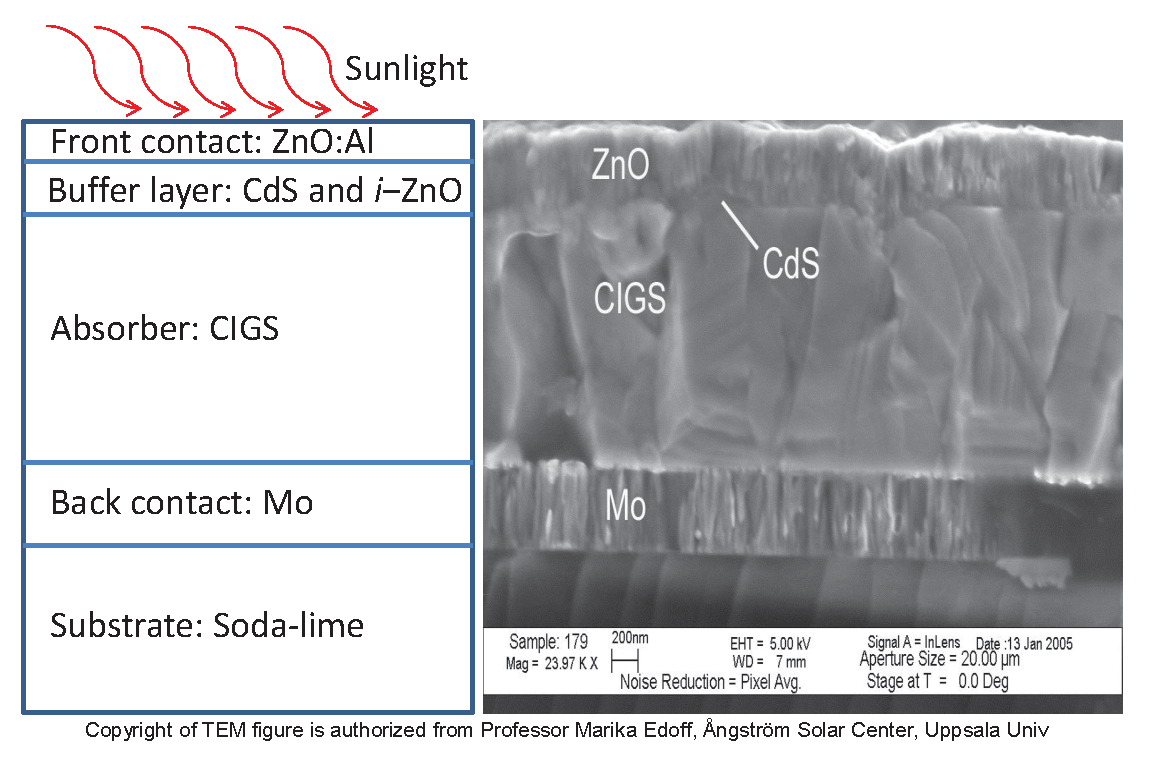
\includegraphics[scale=0.5]{devicestruc.eps} 
\caption{Structure of CIGS solar cell device.}
\label{device}
\end{figure}

Substract is on the bottom, and there are mainly three kinds of substract: soda-lime glass, metal and polyimide. The most common substrate is the one based on soda-lime glass containing sodium (Na) with thickness 
\SI{1} {\mm} to \SI{3} {\mm}. The Na will improve the efficiency and reliablity of the solar cells as well as process tolerance. The molybdenum works as back contact due to its low resistivity and stability at high 
temperature with thickness around \SI{500} {\nm}. The most important part of the device is the \textit{p}-type absorber layer: CIGS, which is dopped by intrinsic defects and around \SI{1500} -- \SI{2000} {\nm}. 
The \textit{n}-type buffer layer CdS is on the top of CIGS, which is around \SI{60} {\nm}. The intrinsic zinc oxide (\textit{i}-ZnO) and \textit{n}-type ZnO layer are followed, and it works as window layer. The \textit{i}-ZnO is to 
avoid the damage of the CIGS and CdS from sputtering damage when depositing the ZnO:Al window layer, and the \textit{n}-type ZnO is dopped by the aluminum (Al) in order to get higher conductivity. 
This CIGS/CdS/ZnO strucutrure was optimized to improve the cell performance.







\chapter{Theory}

\section{Electronic structure calculations }
\label{ch:dft}

\subsection{The quantum many-body problem}
\label{ch:mb}

\noindent A solid material contains a huge number of atoms (around 10\textsuperscript{23} \si{\per\cubic\centi\metre} ), and each atom is constructed by a nucleus and electron(s). 
According to the quantum mechanics principles, all the properties of any system are known if one can figure out a way to solve 
the quantum many-body Schrödinger equation exactly. In this thesis, the time-independent many-body Schrödinger equation is only considered, which is given as

\begin{equation}\label{ssth}
 H^{en} {\Psi^{en}(\{ {\textbf r}_{\textit i}, {\textbf R}_{\textit I} \})} = {E^{en}} {\Psi^{en}(\{ {\textbf r}_{\textit i}, {\textbf R}_{\textit I} \})}.
\end{equation}

Here, term with the superscript "\textit{en}" implies that this term is related with electrons and nuclei. ${\Psi^{en}(\{ {\textbf r}_{\textit i}, {\textbf R}_{\textit I} \})}$ is the exact wavefunction, $\textbf{r}_\textit{i}$ 
and $\textbf{R}_\textit{I}$  stands for coordinators of electron and nucleus, respectively. $E^{en}$ is the system total energy. $H^{en}$ is the Hamiltonian which is defined as

\begin{equation}\label{th}
\begin{split}
& H^{en} = - \sum_i^{Ne} {\frac{\hbar^{2}}{2 m_{\textit e}}}   \nablaia<i> - \sum_I^{Nn} {\frac{\hbar^{2}}{2 m_\textit{I}}} \nablaia<I>  - \sum_i^{Ne} \sum_I^{Nn} \frac{Z_\textit{I}\ e^2}{4 \pi \varepsilon_0 |\textbf{r}_\textit{i}-\textbf{R}_\textit{I}|} \\
& + \frac{1}{2} \sum_i^{Ne} \sum_{j \neq i}^{Ne} \frac{ e^2}{4 \pi \varepsilon_0 |\textbf{r}_\textit{i}-\textbf{r}_\textit{j}|} + \frac{1}{2} \sum_I^{Nn} \sum_{J \neq I}^{Nn} \frac{Z_\textit{I} Z_\textit{J}\  e^2}{4 \pi \varepsilon_0 |\textbf{R}_\textit{I}-\textbf{R}_\textit{J}|}.
\end{split}
\end{equation}

Here, the indices \textit{i}, \textit{j} are used for the electrons, and \textit{I}, \textit{J} are used for atomic nuclei. $Z_I$ implies the charge of the \textit{I}:th nucleus.
$\textit{m}_I$ denotes the nuclear mass, $m_e$ is the electron mass, and $\varepsilon_0$ is vacuum permittivity.

In atomic units, the reduced Planck constant $\hbar$, the electron mass $m_e$, the Bohr radius $a_0$, and the electron charge
$e$ are equal to 1. The Bohr radius is given by the formula $a_0$ = ${\hbar} / {(mc\alpha)}$. Here, $\alpha$ is the fine structure
constant ($\alpha$ = ${e^2}/{(4 \pi \varepsilon_0 c \hbar)}$). Therefore, the velocity of light in atomic units is $c$ = $1/{\alpha}$ and ${e^2}/{(4 \pi \varepsilon_0)}$ = 1. In atomic units, \textbf{Eq. \ref{th}} is given as 

\begin{equation}\label{sth}\begin{split}
&\hath = - \sum_i^{Ne}   \frac{{{\nabla}_{\textit{i}}^{2}}}{2} - \sum_I^{Nn} \frac{{{\nabla}_{\textit{I}}^{2}}}{2 M_\textit{I}}  - \sum_i^{Ne} \sum_I^{Nn} \frac{Z_\textit{I}}{|\textbf{r}_\textit{i}-\textbf{R}_\textit{I}|} \\
& + \frac{1}{2} \sum_i^{Ne} \sum_{j \neq i}^{Ne} \frac{1}{ |\textbf{r}_\textit{i}-\textbf{r}_\textit{j}|} + \frac{1}{2} \sum_I^{Nn} \sum_{J \neq I}^{Nn} \frac{Z_\textit{I} Z_\textit{J}\ }{|\textbf{R}_\textit{I}-\textbf{R}_\textit{J}|}.
\end{split}\end{equation}

Here, $M_I$ is the mass of the \textit{i}:th nucleus in atomic units. The first and second terms are the kinetic energy operator of the electrons and nuclei, respectively.
The other terms are Coulomb interactions between electrons and nuclei, electrons and electrons and nuclei and nuclei in sequence.

One can not solve \textbf{Eq. \ref{ssth}} exactly at present since there are enormous amount of atoms to calculate in reality. More importantly, the exactly form of the wavefunction is unknown.
To approximate the exact solution, one divides it into three different levels generally: the first level is the Born-Oppenheimer approximation; the second level is Hartree,
Hartree-Fock (HF), density functional theory (DFT) and Kohn-Sham (KS) equation; the last level is to solve the secular equation which is an equation that is solved to find the eigenvalue of matrix.

\subsection{The Born-Oppenheimer approximation}
\label{ch:boa}

\textbf{Eq. \ref{ssth}} can be approximated in order to solve it. The first attempt is to seperate the wavefunction of electron and nucleus. Because the Schrödinger Hamiltonian in \textbf{Eq. \ref{sth}} has a couple term between the electron and nucleus, 
thereby one can not do that simply. On the other hand, there exists a small value ${1}/{M_I}$ in \textbf{Eq. \ref{sth}}, which is part of the nucleus kinetic energy
operator term. The reason is that the mass of nucleus is much larger than that of electron, therefore the nuclei are treated as fixed. This indicates that the electrons are seen as interacting under both the external potential caused by nuclei that are fixed in 
some positions and that of the other electrons. 

The separation of motion between electrons and nuclei is called the Born-Oppenheimer approximation. Since the positions of nuclei are fixed, wavefunction can be written as

\begin{equation}\label{nwf}
{\Psi^{en}(\{ {\textbf r}_{\textit i}, {\textbf R}_{\textit I} \})} \   {\approx} \  {\theta(\{{\textbf R}_{\textit I}\})} {\Psi(\{\textbf{r}_{\textit i}\}; \{{\textbf R}_{\textit I}\})}.
\end{equation}

Here, ${\Psi(\{\textbf{r}_{\textit i}\}; \{{\textbf R}_{\textit I}\})}$  is the electrons wavefunction in the Born-Oppenheimer approximation. Since the electrons are under the potential of nuclei, and thus the wavefunction of 
electrons is related with the nucleus postions. 
 
\textbf{Eq. \ref{sth}} can be rewritten as

\begin{equation}\begin{split}\label{nh}
& {H^{en}} = H + H^n \\
& {H}\ = \ {T} \ + \ {U}_{ext} \ + \ {U}_\textit{int}\  \\
& {H^n} = - \sumi<I> \frac{{{\nabla}_{\textit{I}}^{2}}}{2 M_\textit{I}} + {{H}_{zz}}
 \end{split}
\end{equation}

Furthermore, all the unknown terms in \textbf{Eq. \ref{nh}} are defined as

\begin{equation}\begin{split}\label{vext}
& {T} = - \sum_i^{\textit{Ne}}   \frac{{{\nabla}_{\textit{i}}^{2}}}{2} \\
& U_{ext} =  \sum_i^{\textit{Ne}} \sum_J^{\textit{Nn}} \frac{Z_\textit{I}}{|\textbf{r}_\textit{i}-\textbf{R}_\textit{I}|} \\
& {U}_\textit{int} =  \frac{1}{2} \sum_i^{\textit{Ne}} \sum_{j \neq i}^{\textit{Ne}} \frac{1}{ |\textbf{r}_\textit{i}-\textbf{r}_\textit{j}|} \\
& {{H}_{zz}} = \frac{1}{2} \sum_I^{\textit{Nn}} \sum_{J \neq I}^{\textit{Nn}} \frac{Z_\textit{I} Z_\textit{J}\ }{|\textbf{R}_\textit{I}-\textbf{R}_\textit{J}|}.
\end{split}
\end{equation}

Here, $H$ is the Hamiltonian for the electronic system within the Born-Oppenheimer approximation. The subscript $ext$ implies $external$ in \textbf{Eq. \ref{nh}}, and $U_{ext}$ describes
the external potentials interaction. 

Thereby, the new Schrödinger equation combined with \textbf{Eq. \ref{nwf}} and \textbf{Eq. \ref{nh}} is 

\begin{equation}
 \Big( - \sum_I^{\textit{Nn}} \frac{{{\nabla}_{\textit{I}}^{2}}}{2 M_\textit{I}} + {H}_{zz} + {H} \Big) \Big({\theta(\{{\textbf R}_{\textit I}\})} {\Psi(\{\textbf{r}_{\textit i}\}; \{{\textbf R}_{\textit I}\})} \Big) =
 E^{en}(\{{\textbf R_I}\}) \Big({\theta(\{{\textbf R}_{\textit I}\})} {\Psi(\{\textbf{r}_{\textit i}\}; \{{\textbf R}_{\textit I}\})}\Big).
\end{equation}
 
\noindent Here, $E^{en}(\{{\textbf R_I}\})$ is the system total energy, which is ${\textbf R_I}$-dependent because system wavefunction depends on nuclei positions. One ends up with the following equation using \textbf{Eq. \ref{vext}}

\begin{equation}\begin{split}\label{ise}
& {H} {\Psi(\{\textbf{r}_{\textit i}\}; \{{\textbf R}_{\textit I}\})} = E{(\{\textbf{R}_{\textit I}\})} {\Psi(\{\textbf{r}_{\textit i}\}; \{{\textbf R}_{\textit I}\})} \\
& \Big( {H}_{zz1}+{H}_{zz2}+{H}_{zz3}+{H}_{zz}+E(\{{\textbf R}_{\textit I}\}) \Big) {\theta(\{\textbf{R}_{\textit I}\})} = E^{en}(\{{\textbf R_I}\}) {\theta(\{\textbf{R}_{\textit I}\})}.
\end{split}
\end{equation}

\noindent Here, $E{(\{\textbf{R}_{\textit I}\})}$ is the total energy of electronic system, which is also ${\textbf R_I}$-dependent because electrons wavefunction indirectly depends on nuclei positions. The ${H}_{zz1}$,
${H}_{zz2}$, and ${H}_{zz3}$ in \textbf{Eq. \ref{ise}} are derived as

\begin{equation}\begin{split}
 &  {H}_{zz1} = - \sum_I^{\textit{Nn}} \frac{{{\nabla}_{\textit{I}}^{2}}}{2 M_\textit{I}}   \\
 &  {H}_{zz2} = - \sum_I^{\textit{Nn}} \frac{1}{M_\textit{I}} {\int {\Psi'(\{\textbf{r}_{\textit{i}}\}; \{\textbf{R}_{\textit I}\})}^{\ast} {{\nabla}_{\textit{I}}} {{\Psi'(\{\textbf{r}_{\textit{i}} \}; \{\textbf{R}_{\textit I}\})}} d {\textbf r }} {{\nabla}_{\textit{I}}}  \\
 &  {H}_{zz3} = - \sum_I^{\textit{Nn}} \frac{1}{M_\textit{I}} {\int {{\Psi'(\{\textbf{r}_{\textit{i}}\}; \{\textbf{R}_{\textit I}\})}}^{\ast} {{\nabla}_{\textit{I}}^{2}} {{\Psi'(\{\textbf{r}_{\textit{i}} \}; \{\textbf{R}_{\textit I}\})}} d {\textbf r }}. 
\end{split}\end{equation}

From \textbf{Eq. \ref{ise}}, one observes that the lattice dynamical properties of certain system within the Born-Oppenheimer approximation can be obtained. To solve this equation,
the ground state energy $E(\{{{\textbf R}_{\textit I}}\})$ of electronic system is needed. Here, $\{{\textbf R}_{\textit I}\}$ are the parameterized values from the atom position.
 
In summary, the Schrödinger equations of the electrons and nuclei are derived seperately within the Born-Oppenheimer approximation. When one refers to calculations of the ground state properties,
the Schrödinger equation of the electrons is applied (the first line in \textbf{Eq. \ref{ise}}). The Schrödinger equation of nuclei is employed for the calculation of lattice dynamics 
($H_{zz2}$ and $H_{zz3}$ are ignored in the second line in \textbf{Eq. \ref{ise}} normally).

The \textbf{Eq. \ref{ise}} (the first line) is much simpler than \textbf{Eq. \ref{ssth}}. However, it is still not solvable. Further approximations  are needed
to solve this many-body problem.

\subsection{Hartree, Hartree-Fock approximation and density functional theory}

In previous section, the seperation of wavefunction is given within Born-Oppenheimer approximation. The quantum many-body Schrödinger problem becomes the many-electron 
Schrödinger problem. There are two major problems from the Born-Oppenheimer approximation: the first problem is that the number of electron is around 10\textsuperscript{23} \si{\per\cubic\centi\metre}, which is a huge numerical 
problem. However, it is still possible to solve; the second one is that the Hamiltonian includes operators which apply to the single electrons. However, how the wavefunction depends on the single-electron wavefunctions is unknown.
The latter problem can be solved by one of the following three methods: the first method is to figure out a way to seperate or approximate the wavefunction into single-electron function, such as the Hartree and Hartree-Fock (HF) method;
the second method is to find the explict relation bewteen total energy and wavefunction, such as density functional theory (DFT). Within DFT, the system total energy is a functional of electron density which can be constructed by 
wavefunction. Either of these two methods has "pros and cons"; the third one is called Kohn-Sham equation, which is a combination of above two methods. It starts from DFT, however takes advantage of single-electron wavefunctions. 

\subsubsection{Hartree approximation}
\label{ha}
The simplest approximation of the wavefunction for the many-electron Schrödinger equation is the form of acting like independent
electrons. The wavefunction with \textit{N} independent electrons is given as

\begin{equation}\label{wfh}
\wfh = \bwff<1><1> \bwff<2><2> \cdots \bwff<N><N>. 
\end{equation}

Here, $i$ goes through all the electrons. $\bwff<i><i>$ implies state of the $i$:th electron, where the different states of electrons are orthonormalized. From here and following text, the $\textbf R$ is suppressed in the
wavefunction since they are in fixed positions. The variables ${\{\textbf{r}_{\textit{i}}}\}$ include the coordinates of space and spin. The total energy of the electronic system can be written as

\begin{equation}\label{teh}
E^{\textit{H}} = <\wfh |\ {\hath} \ | \wfh  >.
\end{equation}

${\hath}$ can be rewritten as
\begin{equation}\begin{split}
&  {\hath} = \sum_i^{\textit{Ne}} \Big( \frac{{{\nabla}_{\textit{i}}^{2}}}{2} + \sum_I^{\textit{Nn}} \frac{Z_\textit{I}}{|\textbf{r}_\textit{i}-\textbf{R}_\textit{I}|} \Big) +   \frac{1}{2} \sum_i^{\textit{Ne}} \sum_{j \neq i}^{\textit{Ne}} \frac{1}{ |\textbf{r}_\textit{i}-\textbf{r}_\textit{j}|} \\
& = \sum_i^{\textit{Ne}} h_1(\textbf{r}_\textit{i}) + \frac{1}{2} \sum_i^{\textit{Ne}} \sum_{j \neq i}^{\textit{Ne}} h_2(\textbf{r}_\textit{i},\textbf{r}_\textit{j}).
\end{split}
\end{equation}

Therefore, the total energy of system is given by making the substitution using \textbf{Eq. \ref{nh}} and \textbf{Eq. \ref{wfh}} into \textbf{Eq. \ref{teh}}
\begin{equation}\begin{split}
& E^\textit{H} = \sum_i^{\textit{Ne}} <\bwff<i><i> | \  h_1(\textbf{r}_\textit{i}) \ | \bwff<i><i> > \\
& +\frac{1}{2} \sum_i^{\textit{Ne}} \sum_{j \neq i}^{\textit{Ne}} <\bwff<i><i> \bwff<j><j>|\ h_2(\textbf{r}_\textit{i},\textbf{r}_\textit{j}) \ | \bwff<i><i> \bwff<j><j>>.  
\end{split}\end{equation}

In order to calculate the stationary state with the lowest energy of the system, the functional differentiation with respect to infinitesimal change of any wavefunction $\phi_{k}(\textbf{r})$ should be
zero. That is, 
\begin{equation}
 \phi_{k}(\textbf{r}) \rightarrow \phi_{k}(\textbf{r}) + \delta \phi_{k}(\textbf{r})  \Rightarrow \delta E^{\textit{H}} = 0.
\end{equation}

Furthermore, the constraint is that the different states of electrons are orthonormalized. According to method of Lagrange multipliers, the variation with respect to any wavefunction $\phi^*_{k}(\textbf{r})$ and  Lagrange multiplier $E_{i,j}^{H}$ is satisfied

\begin{equation}\begin{split}\label{haa}
 \frac{ \delta  \Big(E^{\textit{H}} - \sum_i^{\textit{Ne}} \sum_j^{\textit{Ne}} E_{i,j}^{H} (<\bwff<i><i> | \bwff<j><j>> -\ \delta_{ij})\Big)}{\delta \phi^*_{k}(\textbf{r})}  = 0. 
\end{split}
\end{equation}


Here, $\phi_{k}(\textbf{r})$ also can be utilized, however, variation with respect to $\phi^*_{k}(\textbf{r})$ and $\phi_{k}(\textbf{r})$ are equivalent. The result is more organized using $\phi^*_{k}(\textbf{r})$.

$\delta E^{\textit{H}}$ in \textbf{Eq. \ref{haa}} can be calculated by two parts. The first part is 

\begin{equation}\begin{split}\label{hartree1}
&  \delta ( \sum_i^{\textit{Ne}} <\bwff<i><i> |\ h_1(\textbf{r}_\textit{i})  \ | \bwff<i><i> > )  \\
& =  < \delta \phi_{\textit{k}}(\textbf{r}_\textit{}) |\ h_1(\textbf{r}_\textit{})  \ |  \phi_{\textit{k}}(\textbf{r}_\textit{}) >  +  < \phi_{\textit{k}}(\textbf{r}_\textit{}) |\ h_1(\textbf{r}_\textit{})  \ | \delta \phi_{\textit{k}}(\textbf{r}_\textit{}) > 
\end{split}\end{equation}

The second part is

\begin{equation}\begin{split}\label{hartree2}
& \frac{1}{2} \delta \sum_i^{\textit{Ne}} \sum_{j \neq i}^{\textit{Ne}} <\bwff<i><i> \bwff<j><j>|\ h_2(\textbf{r}_\textit{i},\textbf{r}_\textit{j}) \ | \bwff<i><i> \bwff<j><j>> \\
& = \frac{1}{2}  \sum_{i \neq k}^{\textit{Ne}} \Big( <\bwff<i><i>  \delta \bwff<k><>|\ h_2(\textbf{r}_\textit{i},\textbf{r}_\textit{}) \ | \bwff<i><i> \bwff<k><>> \\
& + <\bwff<i><i>  \bwff<k><>|\ h_2(\textbf{r}_\textit{i},\textbf{r}_\textit{}) \ | \bwff<i><i> \delta \bwff<k><>> \Big) \\
& + \frac{1}{2}  \sum_{j \neq k}^{\textit{Ne}} \Big( <\delta \bwff<k><>  \delta \bwff<j><j>|\ h_2(\textbf{r}_\textit{},\textbf{r}_\textit{j}) \ | \bwff<k><> \bwff<j><j>> \\
& + < \bwff<k><>  \bwff<j><j>|\ h_2(\textbf{r}_\textit{},\textbf{r}_\textit{j}) \ | \delta \bwff<k><> \bwff<j><j>> \Big) \\
& =   \sum_{i \neq k}^{\textit{Ne}} \Big( <\bwff<i><i>  \delta \bwff<k><>|\ h_2(\textbf{r}_\textit{i},\textbf{r}_\textit{}) \ | \bwff<i><i> \bwff<k><>> \\
& + <\bwff<i><i>  \bwff<k><>|\ h_2(\textbf{r}_\textit{i},\textbf{r}_\textit{}) \ | \bwff<i><i> \delta \bwff<k><>> \Big) 
\end{split}\end{equation}

Here, the factor of $\frac{1}{2}$ cancels because the \textit{2}nd (\textit{3}rd) line is the same with \textit{4}th (\textit{5}th) line in \textbf{Eq. \ref{hartree2}} due to the exchangeable of the index of $i$ and $j$. 

To get the final solution, one more calculation is given as 

\begin{equation} \begin{split}\label{xixihaha}
& \delta \sum_i^{\textit{Ne}} \sum_j^{\textit{Ne}} E_{i,j}^{\textit{H}} \Big(<\phi_{i}(\textbf{r}_\textit{i}) | \phi_{j}(\textbf{r}_\textit{j}) > - \ \delta_{i,j}\Big) \\
& = \sum_j^{\textit{Ne}} E_{k,j}^{\textit{H}} \Big(< \delta \phi_{k}(\textbf{r}) | \phi_{j}(\textbf{r}_\textit{j}) > \Big) + \sum_i^{\textit{Ne}} E_{i,k}^{\textit{H}} \Big(<\phi_{i}(\textbf{r}_\textit{i}) | \delta \phi_{k}(\textbf{r}_\textit{}) >\Big) \\
& = \sum_i^{\textit{Ne}} E_{k,i}^{\textit{H}} \Big(< \delta \phi_{k}(\textbf{r}) | \phi_{i}(\textbf{r}_\textit{i}) >  + <\phi_{i}(\textbf{r}_\textit{i}) | \delta \phi_{k}(\textbf{r}_\textit{}) >\Big)
\end{split}
\end{equation}


Therefore, \textbf{Eq. \ref{haa}} can be derived as 

\begin{equation}\label{hartreq11}
\Big(-\frac{\nabla^{2}_{k}}{2} + \sum_I^{\textit{Nn}} \frac{Z_\textit{I}}{|\textbf{r}_\textit{}-\textbf{R}_\textit{I}|} + \sum_{j \neq k}^{\textit{Ne}}  <\bwfn<j><'>\ | \frac{1}{|\textbf{r} - \textbf{r}^{'} |} \ | \bwfn<j><'>>\Big) \bwff<k><> = \sum_i^{\textit{Ne}} E_{k,i}^{H} \bwff<i><> 
\end{equation}

There are many solutions to \textbf{Eq. \ref{hartreq11}}, each corresponding to a different set of $E_{k,i}^{H}$. One can choose to $E_{k,i}^{H}$ which satisfies $E_{k,i}^{H}$ = $\delta_{k,i}\epsilon_k^{\textit{H}}$. The \textbf{Eq. \ref{hartreq11}}
can be rewriteen as

\begin{equation}\begin{split}\label{hartreq}
& \Big(-\frac{\nabla^{2}_{k}}{2} + \sum_I^{\textit{Nn}} \frac{Z_\textit{I}}{|\textbf{r}_\textit{}-\textbf{R}_\textit{I}|} + \sum_{j \neq k}^{\textit{Ne}}  <\bwfn<j><'>\ | \frac{1}{|\textbf{r} - \textbf{r}^{'} |} \ | \bwfn<j><'>>\Big) \bwff<k><> = \epsilon_k^{\textit{H}} \bwff<k><>  \\
&  \qquad \qquad \qquad  \qquad \qquad \qquad \qquad \qquad  \Downarrow  \\
& \Big(-\frac{\nabla^{2}_{i}}{2} + \sum_I^{\textit{Nn}} \frac{Z_\textit{I}}{|\textbf{r}_\textit{}-\textbf{R}_\textit{I}|} + \sum_{j \neq i}^{\textit{Ne}}  <\bwfn<j><'>\ | \frac{1}{|\textbf{r} - \textbf{r}^{'} |} \ | \bwfn<j><'>>\Big) \bwff<i><> = \epsilon_i^{\textit{H}} \bwff<i><>  \\
\end{split}
\end{equation}


Here, \textbf{Eq. \ref{hartreq}} is a group of dependent single particle equations. $\epsilon_k^{\textit{H}}$ is identified as the eigenvalue for this single-electron Hartree equation.

\subsubsection{Hartree-Fock approximation}
Hartree approximation is the simplest approximation, while Hartree-Fock approximation is the method which considers the antisymmetry of the wavefunction. It is shown as

\begin{equation}\label{hfwf}
\Psi^\textit{HF} ( \cdots \textbf{r}_\textit{i} \cdots  \textbf{r}_\textit{j} \cdots ) = - \Psi^\textit{HF} ( \cdots \textbf{r}_\textit{j} \cdots  \textbf{r}_\textit{i} \cdots).
\end{equation}

Here, each variable ${\textbf{r}_{\textit{i}}}$ includes the coordinates of space and spin. Slater introduced an way to construct the wavefunction subject to \textbf{Eq. \ref{hfwf}}. The wavefunction of the many-electron 
Schrödinger equation is described in a matrix determinant for the $N$ number of electrons (for aesthetical reason, $N$ implies the number of electrons and not $Ne$ in the section)

\begin{equation}\label{hfwfm}
\Psi^\textit{HF}(\mathbf{r}_1, \mathbf{r}_2, \ldots, \mathbf{r}_N) =
\frac{1}{\sqrt{N!}} \left|
\begin{matrix}
    \bwff<1><1> & \bwff<2><1> & \cdots & \bwff<N><1> \\
    \bwff<1><2> & \bwff<2><2> & \cdots & \bwff<N><2> \\
    \vdots               & \vdots               &        & \vdots               \\
    \bwff<1><N> & \bwff<2><N> & \cdots & \bwff<N><N>
\end{matrix} \right|.
\end{equation}
\noindent Here, the factor in front ensures normalization, $i$ goes through all the electrons, and $\bwff<i><i>$ implies state of the ($i$):th electron. If two rows in \textbf{Eq. \ref{hfwfm}} are exchanged, the result is agreed 
with \textbf{Eq. \ref{hfwf}}.

The total energy of Hartree-Fock approximation, which can be determined similarly as in the previous section of Hartree approximation, is given as

\begin{equation}\begin{split}
&E^\textit{HF} = \sum_i^{\textit{N}} <\bwff<i><> |\ -\frac{\nabla^{2}_{i}}{2} + \sum_I^{\textit{Nn}} \frac{Z_\textit{I}}{|\textbf{r}_\textit{}-\textbf{R}_\textit{I}|}  \ | \bwff<i><> > \\
& + \frac{1}{2} \sum_i^{\textit{N}} \sum_j^{\textit{N}} <\bwff<i><> \bwfn<j><'>|\ \frac{1}{|\textbf{r} - \textbf{r}^{'} |} \ | \bwff<i><> \bwfn<j><'>> \\
& - \frac{1}{2} \sum_i^{\textit{N}} \sum_j^{\textit{N}} <\bwfn<i><'> \bwfn<j><>|\ \frac{1}{|\textbf{r} - \textbf{r}^{'} |} \ | \bwfn<i><> \bwfn<j><'>>.
\end{split}\end{equation}

Here, there is no contribution to the sum when \textit{i} = \textit{j}. In the same mathematical way as in previous section but somewhat more complicated, the single particle Hartree-Fock equation can be obtained

\begin{equation}\begin{split}\label{above1}
& \{ -\frac{\nabla^{2}_{\textit i}}{2} + \sum_I^{\textit{Nn}} \frac{Z_\textit{I}}{|\textbf{r}_\textit{}-\textbf{R}_\textit{I}|} + \sum_{j}^{\textit{N}} <\bwfn<j><'>\ | \frac{1}{|\textbf{r} - \textbf{r}^{'} |} \ | \bwfn<j><'>> \} \bwff<i><>  \\
& - \sum_{j}^{\textit{N}}  < \bwfn<j><'>|\ \frac{1}{|\textbf{r} - \textbf{r}^{'} |} \ | \bwfn<i><'> >) \bwfn<j><>  = \epsilon_{i}^{\textit{HF}} \bwff<i><>.
\end{split}\end{equation}

In comparison with Hartree equation in \textbf{Eq. \ref{hartreq}}, there is an extra term in the \textbf{Eq. \ref{above1}}, which is so called exchange term. In order to show the equation in a more organized way,
\textbf{Eq. \ref{above1}} is equivalent to

\begin{equation}\label{aaaaa}\begin{split}
\{ -\frac{\nabla^{2}_{\textit i}}{2} +  \sum_I^{\textit{Nn}} \frac{Z_\textit{I}}{|\textbf{r}_\textit{}-\textbf{R}_\textit{I}|} +V_\textit{HF}(\textbf{r}) \}  \bwff<i><>  = \epsilon_{i}^{\textit{HF}}   \bwff<i><>.
\end{split}\end{equation}

\begin{equation}
\begin{split}
&  V_\textit{HF}(\textbf{r})= \int \frac{\rho(\textbf{r}{'}) - \rho_{\textit{i}}^{\textit{HF}}(\textbf{r},\textbf{r}{'})}{|\textbf{r} - \textbf{r}^{'} |}  \mathrm{d}\textbf{r}^{'} \\
& \rho_{\textit{i}}^{\textit{HF}}(\textbf{r},\textbf{r}{'}) = \sum_j^N \frac{\phi_{i}^{}(\textbf{r}{'}) \phi_{i}^{*}(\textbf{r}{}) \phi_{j}^{}(\textbf{r}{}) \phi_{j}^{*}(\textbf{r}{'})} {\phi_{i}^{}(\textbf{r}) \phi_{i}^{*}(\textbf{r})}  \\
& \rho(\textbf{r}) = \sum_i^N  {|\bwff<i><>|}^{2}.
\end{split}
\end{equation}


\subsubsection{Density functional theory}
The Hartree and Hartree-Fock (HF) methods are very classic methods to solve the many-electron Schrödinger equation. However, the HF method only includes the exchange term and not the electron correlation term. It is not suitable 
for the solid materials. Apart from the Hartree and HF method, there is a modern method to solve the more complicated calculations of electron system, namely density functional theory (DFT). 
It is introduced by Hohenberg and Kohn in 1964, moreover, Kohn and Pople was awarded Chemistry Nobel Prize in 1998.

The idea of the DFT is to treat the electron density in solid materials instead of using the many-particle wavefunction. One can benefit that the degree of freedom reduces from 3\textit{N} (\textit{N} is the number of electrons) to 3. It is apparently less 
complicate than those of Hartree and HF methods. 

$\textbf{The density as basic variable}$ 

There are two questions coming out if considering the electron density as the role of wavefunction. The first one is whether it is the equivalence relation between the electron density and wavefunction in the electron system. 
The second one is how to solve the problem if considering the electron density instead of the wavefunction. In order to explain above two questions, there are two very basic theorems introduced by Hohenberg and Kohn:

\begin{thm}
\label{hk1}
\noindent The first theorem states that the external potential $V_\textit{ext}(\textbf{r})$  is determined uniquely for any electron system by the ground-state electron density $\rho$.
\end{thm}

The above theorem indicates that all the ground state properties are determined by the true ground-state density $\rho$ as well,
such as, the total energy \textit{E} = \textit{E}[$\rho$]. 

The above theorem also explains the equivalence relation between the electron density and wavefunction. Because Hamiltonian is obtained from external potential,
then the wavefunction is obtained. Therefore the corresponding electron density is determined. Moreover, from the theorem, the external potential is unique decided by electron
density. Therefore the electron density contains the same information as the wavefunction.

The proof of the theorem is given. Let us assume that there exsits two external potentials named $V_\textit{ext}(\textbf{r})$ and $V'_\textit{ext}(\textbf{r})$ leading to the same ground state 
electron density $\rho$. Obviously, this will lead to two different Hamiltonians, that is, ${H}$ and ${H'}$, as well as two different corresponding
wavefunctions named $\Psi$ and $\Psi'$. Since $\Psi$ are not the ground state wavefunction of ${H'}$, the same rules to $\Psi'$ and ${H}$, two following
inequality equations are satisfied



\begin{equation}\label{hkpf1}\begin{split}
&  E = \langle \Psi\ |{H}|\ \Psi \rangle  \ < \  \langle \Psi'\ |{H}|\ \Psi' \rangle,\\
&  E' = \langle \Psi'\ |{H'}|\ \Psi' \rangle  \ < \  \langle \Psi\ |{H'}|\ \Psi \rangle.
\end{split}\end{equation}

Taking advangtage of the Hamiltonian from \textbf{Eq. \ref{nh}} ($V_\textit{ext}(\textbf{r})$ instead of $U_{\textit{ext}}$), the following equation is derived
\begin{equation}\label{hkpf2}\begin{split}
&    \langle \Psi'\ |{H}|\ \Psi' \rangle \\
&  = \langle \Psi'\ |{H'} + {H} - {H'}|\ \Psi' \rangle \\
&  = \langle \Psi'\ |{H'} |\Psi' \rangle + \langle \Psi' | {H} - {H'}|\ \Psi' \rangle \\
&  = E' + \int d \textbf{r} \Big( V_\textit{ext}(\textbf{r}) - V'_\textit{ext}(\textbf{r}) \Big)  \rho(\textbf{r}).
\end{split}\end{equation}

Using \textbf{Eq. \ref{hkpf1}} and \textbf{Eq. \ref{hkpf2}}, the following relation is given by

\begin{equation}\label{hkpf3}
 E  < \  E' + \int d \textbf{r} \Big( V_\textit{ext}(\textbf{r}) - V'_\textit{ext}(\textbf{r}) \Big)  \rho(\textbf{r}).
\end{equation}

Another similar inequality equation can be gained if one changes the equation $\langle \Psi\ |{H'}|\ \Psi \rangle$ like \textbf{Eq. \ref{hkpf2}}
\begin{equation}\label{hkpf44}
  E'  < \  E + \int d \textbf{r} \Big( V'_\textit{ext}(\textbf{r}) - V_\textit{ext}(\textbf{r}) \Big)  \rho(\textbf{r}).
\end{equation}

Plus the left side and right side from both \textbf{Eq. \ref{hkpf3}} and \textbf{eq. \ref{hkpf44}}, a contradictory result is given as
\begin{equation}\label{hkpf4}
  E + E'  < \  E' + E.
\end{equation}

Since this is an incorrect relation, the external potential $V_\textit{ext}(\textbf{r})$ has to be unique.

\begin{thm}
\label{hk2}
\noindent The second theorem states that there is a universal functional $F[\rho]$ for the total energy in the terms of the electron density $\rho$ with any external potential $V_\textit{ext}(\textbf{r})$ ,
and the exact ground-state density is gained when the ground state total energy functional reaches its minimal value, that is, E[$\rho'$]>E[$\rho$]. Here, $\rho$ is the exact ground-state density.
\end{thm}

The proof of theorem is given. Because of the first theorem, the total energy can be expressed in the following way (ignoring the interaction between nuclei)
\begin{equation}\label{hkpf5}\begin{split}
& E[\rho] \ = \langle \Psi  | \ {T} \ + \ {V}_\textit{int}  \ + \ {V}_\textit{ext} \ | \Psi \rangle \\
&     = \langle \Psi  | \ {V}_\textit{ext} \ | \Psi \rangle  + \underbrace{\langle \Psi  | \ {T} \ + \ {V}_\textit{int}  \ \ | \Psi \rangle}  \\
&     =   \ \int \rho(\textbf{r}) V_\textit{ext} \qquad +  \qquad F[\rho]. 
\end{split}
\end{equation}

In \textbf{Eq. \ref{hkpf5}}, the term of $F[\rho]$ is the universal functional for all the many-electron system.

The functional of total energy $E[\rho']$ reach the minimum at the exact ground-state electron density $\rho$
\begin{equation}\begin{split}
 & E[\rho'] \ =   \ \int \rho'(\textbf{r}) V_\textit{ext}  + \  F[\rho'] > E[\rho]. 
\end{split}
\end{equation}
 


From above equation, one knows the total energy for the case of exact ground-state electron density is lower than any other cases. It also generates that one can achive
the exact ground-state electron density by minimizing the total energy.



From those two theorems, one knows how to solve this problem theoretically. However in practice, $E[\rho]$ is unknown. 
Therefore, one more method is needed to solve it, which is so called Kohn-Sham (KS) equation.

\subsubsection{Kohn-Sham equation}

The Hartree and Hartree-Fock methods are introduced to solve the many-body problem, both of which are based on the idea of transforming complex 
many-electron problem to single-electron problem by using different wavefunctions. The DFT only consider to take use of information from Hamiltonian, however not solvable. 
Therefore, it is best to combine these two ideas together. The DFT is solved by Kohn-Sham equation introduced by Kohn and Sham in 1965,
which is constructed in the following text (ignoring the interaction between nuclei).

Assume that the exact ground-state density is obtained by the wavefunction $\wfks = \bwf<1><1> \bwf<2><2> \cdots \bwf<M><M>$. Here, \textit{M} is a number which is 
less than $10^{23}$ a lot and $\bwf<i><i>$ is auxiliary independent single-electron wavefuntion, and electron density is defined as

\begin{equation}\label{ks1}
 \rho(\textbf{r}) = \sumi<i> {\Psi^{\textit{KS}*}_{i}(\textbf{r})} {\Psi^{\textit{KS}}_{i}(\textbf{r})}.
\end{equation}

If the density is exact, thereby the total energy is defined exactly. It is given as

\begin{equation}\label{kse}
\begin{split}
&E[\rho] \ =\ T[\rho] \ + \ V_\textit{int}[\rho] \ + \ V_\textit{ext}[\rho]  \\
&\ \ \   = \ T_{0}[\rho] \ + \ V_\textit{HF}[\rho] \ + V_\textit{ext}[\rho]+\underbrace{\ (T[\rho] \ - \ T_{0}[\rho]) \ + \  (V_\textit{int}[\rho] \ - \ V_\textit{HF}[\rho])\ }       \\
&\ \ \   = \ T_{0}[\rho] \quad \,  + \quad \,  V_\textit{HF}[\rho] \quad \, + \quad \, V_\textit{ext}[\rho] \quad \, + \quad \, V_\textit{c}[\rho].
\end{split}
\end{equation}

Here, $E[\rho]$  is the total energy, and $\rho$ is the ground-state density. $T[\rho]$, $V_\textit{int}[\rho]$ and $V_\textit{ext}[\rho]$ in order are the energy from external potential, the exact kinetic, 
and the exact electron-electron potential energy. $T_{0}[\rho]$ is the kinetic energy of independent electrons, $V_\textit{HF}[\rho]$ is the potential from the Hartree-Fock approximation, and $V_\textit{c}[\rho]$
denotes correlation energy.

From the Hartree-Fock approximation, one can further know that
\begin{equation}
 V_\textit{HF}[\rho] \ = \ V_\textit{H}[\rho] \ + \ V_\textit{x}[\rho].
\end{equation}

Here, $V_\textit{H}[\rho]$ and $ V_\textit{x}[\rho] $ are the Hartree contribution and exchange contribution, respectively. Thereby, the \textbf{Eq. \ref{kse}} can be further defined as

\begin{equation}\label{ccc}
\begin{split}
&E[\rho]\ = \ T_{0}[\rho] \ + \ V_\textit{H}[\rho] \ + \ V_\textit{ext}[\rho] \ + \ \underbrace{\ V_\textit{x}[\rho]  \ + \ V_\textit{c}[\rho]}  \\
&\ \ \ = \ T_{0}[\rho] \quad + \quad V_\textit{H}[\rho] \quad + \quad V_\textit{ext}[\rho] \quad + \quad V_\textit{xc}[\rho].
\end{split}\end{equation}

Here, $V_\textit{xc}[\rho]$  is the exchange-correlation term. From \textbf{Eq. \ref{kse}}, one does not know the explicit expression of $V_\textit{xc}[\rho]$. However, the first three terms are give as

\begin{equation}
 T_{0}[\rho]\ = \sum_{i}\ < \Psi_{i}^{\textit{KS}}(\textbf{r}) \ | -\frac{\nabla^{2}_{i}}{2} \ | \Psi_{i}^{\textit{KS}}(\textbf{r}) >
\end{equation}

\begin{equation}
V_\textit{H}[\rho] \ = \ \frac{1}{2} \int \int \mathrm{d} {\textbf{r}} \mathrm{d}{\textbf{r}^{\prime}} \frac{\rho({\textbf{r}})\rho(\textbf{r}^{\prime})}{|{\textbf{r}}-{\textbf{r}}^{\prime}|}
\end{equation}

\begin{equation}
V_\textit{ext}[\rho]\ = \ \int \mathrm{d}{\textbf{r}} \rho(\textbf{r}) V_\textit{ext}(\textbf{r}). 
\end{equation}

In order to derive the ground state properties in the many-electron system, one can view this problem as the process of minimizing the total energy by varying the wavefunction $\Psi^{\textit{KS}*}_{\textit{i}}(\textbf{r})$. Since
 the wavefunction can be constructed to electron density (\textbf{Eq. \ref{ks1}}), just like the derivation in the section of Hartree approximation, finally one can get the Kohn-Sham equation

\begin{equation}\label{aaa}
 \Big(-\frac{\nabla^{2}_{i}}{2}\ + \ V^\textit{KS}(\textbf{r})\Big) \Psi^{\textit{KS}}_{\textit{i}}(\textbf{r}) = E^{\textit{KS}}_{\textit{i}} \Psi^{\textit{KS}}_{\textit{i}}(\textbf{r}).
\end{equation}

Here,

\begin{equation}\begin{split}
&\ V^\textit{KS}(\textbf{r}) \ = \ V_\textit{ext}(\textbf{r}) + \int \mathrm{d}{\textbf{r}^{\prime}}  \frac{\rho(\textbf{r}^{\prime})}{|{\textbf{r}}-{\textbf{r}}^{\prime}|} \ + \ \frac{\delta{V_\textit{xc}}}{\delta{\rho(\textbf{r})}} \\
&\ = \ \ V_\textit{ext}(\textbf{r}) + \int \mathrm{d}{\textbf{r}^{\prime}}  \frac{\rho(\textbf{r}^{\prime})}{|{\textbf{r}}-{\textbf{r}}^{\prime}|} \ + \ \upsilon_\textit{xc}(\textbf{r}).
\end{split}
\end{equation}

One can think of the Hamiltonian in another point of view, that is, single particle system with three different potentials. 

There is no total energy equation expression yet. However, if one changes the \textbf{Eq. \ref{aaa}} as 
\begin{equation}\label{bbb}
\sumi<i> \Psi^{\textit{KS}*}_{\textit{i}}(\textbf{r}) \Big(-\frac{\nabla^{2}_{i}}{2}\ + \ V^\textit{KS}(\textbf{r})\Big) \Psi^{\textit{KS}}_{\textit{i}}(\textbf{r}) = \sumi<i> \Psi^{\textit{KS}*}_{\textit{i}}(\textbf{r}) E^{\textit{KS}}_{\textit{i}} \Psi^{\textit{KS}}_{\textit{i}}(\textbf{r}).
\end{equation}

Based on \textbf{Eq. \ref{ccc}} and \textbf{Eq. \ref{bbb}}, the total energy expression is
\begin{equation}\label{totalenergy}
\begin{split}
& E = \sumi<i> E^{\textit{KS}}_{\textit{i}} - \ \frac{1}{2} \int \int \mathrm{d} {\textbf{r}} \mathrm{d}{\textbf{r}^{\prime}} \frac{\rho({\textbf{r}})\rho(\textbf{r}^{\prime})}{|{\textbf{r}}-{\textbf{r}}^{\prime}|} \\
&    + \ V_\textit{xc}[\rho] - \int   \upsilon_\textit{xc}(\textbf{r}) \rho({\textbf{r}}).
\end{split}
\end{equation}

So far there are two problems still in the air: one is the exact format of $\upsilon_\textit{xc}(\textbf{r})$; the other one is how to solve the Kohn-Sham equation.

\subsubsection{The exchange-correlation potential}

The exchange-correlation potential is the most difficult part during the process of solving the Kohn-Sham equation, because it is still unknown yet. Therefore, there
 are varies of approximations about it, such as, the local density approximation (LDA), generalized-gradient approximation (GGA) and many others.

$\textbf{The local density approximation}$

The local density approximation is the simplest way to approximate the exchange-correlation part. The idea is that the value 
of the exchange-correlation potential in the very tiny small volume is equal to the homogeneous electrons with the same density in 
the volume, the explicit equation is

\begin{equation}
 E^\textit{LDA}_\textit{xc} = \int \rho(\textbf{r}) \varepsilon_\textit{xc}( \rho(\textbf{r}) ) \mathrm{d} \textbf{r}.
\end{equation}

Here, $ E^\textit{LDA}_\textit{xc} $ is the exchange-correlation energy functional for the LDA, $\rho(\textbf{r})$ is the charge density, $\varepsilon_\textit{xc}$ is homogeneous 
electrons gas with variable of  $\rho(\textbf{r})$ .

The $\varepsilon_\textit{xc}$ is an ideal state within a solid, which assumes that the charge is homogeneously all over the space

\begin{equation}
 \rho(\textbf{r}) = \rho = \frac{N}{V}.
\end{equation}

Here, $N$ is number of electrons within the solid, and $V$ is the volume of solid.
 not functional. 

$\textbf{The generalized gradient approximation}$

The GGA is the approximation beyond the LDA, which incorporates not only the density within the tiny volume, but also the gradient
 of the density. The explicit equation is

\begin{equation}
E^{\textit{GGA}}_{\textit{xc}}\ = \ \int \rho(\textbf{r}) \varepsilon_\textit{xc}( \rho(\textbf{r}), \nabla \rho(\textbf{r}) ) \mathrm{d} \textbf{r}.
\end{equation}

Here, $E^{\textit{GGA}}_{\textit{xc}}$ is the exchange-correlation energy functional for the GGA, $\nabla \rho(\textbf{r})$ is the gradient  of charge density in the position of \textbf{r}.

Today, there exists hundreds of different potentials. It is stll ongoing development. The advangtage of Kohn-Sham is that one new potential is implemented easily. In the sam time, the number of potential is huge due to
the simplicity of implementation.

\subsection{Solving the secular equation}

The process for solving Kohn-Sham equation can be achived by iteration as well. However, the difference between solving Kohn-Sham 
equation and Hartree or Hartree-Fock equation is that the wavefunction is replaced by the electron density in Kohn-Sham equation. Thereby, an initial 
electron density is defined at the beginning of the calculation, then the equation is solved iteratively until the reasonable solution is obtained.

%%%%%%%%%%%%%%%%%%%%figure
\tikzstyle{decision} = [diamond, draw, fill=white!20,
    text width=10em, text badly centered, node distance=2.5cm, inner sep=0pt]
\tikzstyle{block} = [rectangle, draw, fill=white!20,
    text width=12em, text centered, rounded corners, minimum height=3em]
\tikzstyle{line} = [draw, very thick, color=black!50, -latex']

\begin{figure}[H]
\centering
\begin{tikzpicture}[scale=0.6 , node distance = 2.5cm,transform shape]
    % Place nodes
    \node [block] (init) {Initialize};
    \node [block, below of=init] (potential) {Calculate potential $V( {\textbf r})$};
    \node [block, below of=potential, node distance=2.5cm] (KS) {Solve Kohn-Sham equation};
    \node [block, below of=KS, node distance=2.5cm] (fermi) {Calculate Fermi energy $E_F$};
    \node [block, below of=fermi, node distance=2.5cm] (density) {Calculate new density $\rho^{new}$};
    \node [block, left of=fermi, node distance=6cm] (update) {Determine the mix density $\rho^{i+1} = F (\rho^{i}, \rho^{new}) $};
    \node [decision, below of=density, node distance=3.8cm] (converge) {Converged?};
    \node [block, below of=converge, node distance=3.8cm] (done) {Finished};
    % Draw edges
    \path [line] (init) -- (potential);
    \path [line] (potential) -- (KS);
    \path [line] (KS) -- (fermi);
    \path [line] (fermi) -- (density);
    \path [line] (density) -- (converge);
    \path [line] (converge) -| node [pos=0.2, above, color=black] {No} (update);
    \path [line] (update) |- (potential);
    \path [line] (converge) -- node [pos=0.2, right, color=black] {Yes}(done);

\end{tikzpicture}
\caption{Flow chart of the ${\textit {(i+1)}}$:th iterations for solving Kohn-Sham equation.}
\label{fig:bo}
\end{figure}




Here, $\rho^{i}$ and $\rho^{i+1}$are the charge density of the $\textit{(i)}$:th and $\textit {(i+1)}$:th iteration solving Kohn-Sham equation, respectively.

\vspace{100cm}

\subsection{Eigenvalue problem}

In order to solve \textbf{Eq. \ref{aaa}}, the Kohn-Sham equation can be transformed into the general eigenvalue problem. If the Kohn-Sham equation is given as (ignore the index  in wavefunction compared with \textbf{Eq. \ref{aaa}})

\begin{equation}\label{ep2}
 \hath \Psi^{KS} (r) = E \Psi^{KS} (r).
\end{equation}
 

The wavefunction is defined as

\begin{equation}\label{ep1}
 \Psi^{KS} (r) = \sum\limits_j^N C_j \Phi_j (r).
\end{equation}
 
Here, $C_j$ is a complex number, and $\Phi_j (r)$ is the basis function of wavefunction. 


If \textbf{Eq. \ref{ep1}} is plugged into \textbf{Eq. \ref{ep2}}, and left multiply $\Phi^*_1, \Phi^*_2, \cdot, \Phi^*_N$ in order, finally it will end up with a set of equations

\begin{equation}\begin{split}\label{ep3}
\left[
\begin{matrix}
    \Phi^*_1 \hath \Phi_1 & \Phi^*_1 \hath \Phi_2 & \cdots & \Phi^*_1 \hath \Phi_N \\
    \Phi^*_2 \hath \Phi_1 & \Phi^*_2 \hath \Phi_2 & \cdots & \Phi^*_2 \hath \Phi_N \\
    \vdots               & \vdots               &        & \vdots               \\
    \Phi^*_N \hath \Phi_1 & \Phi^*_N \hath \Phi_2 & \cdots & \Phi^*_N \hath \Phi_N \\
\end{matrix} \right] \left[ \begin{array}{c} C_1 \\ C_2 \\ \vdots \\ C_N\end{array} \right] \\
= E \left[
\begin{matrix}
    \Phi^*_1 \Phi_1 & \Phi^*_1 \Phi_2 & \cdots & \Phi^*_1 \Phi_N \\
   \Phi^*_2 \Phi_1 & \Phi^*_2 \Phi_2 & \cdots & \Phi^*_2 \Phi_N \\
    \vdots               & \vdots               &        & \vdots               \\
   \Phi^*_N \Phi_1 & \Phi^*_N \Phi_2 & \cdots & \Phi^*_N \Phi_N \\
\end{matrix} \right]\left[ \begin{array}{c} C_1 \\ C_2 \\ \vdots \\ C_N\end{array} \right].
\end{split}\end{equation}

If $H_{ij} = \Phi^*_i \hath \Phi_j$ and $S_{ij} = \Phi^*_i \Phi_j$ are defined, then the \textbf{Eq. \ref{ep3}} becomes

\begin{equation}\begin{split}\label{ep467}
\left[
\begin{matrix}
    H_{11} & H_{12} & \cdots & H_{1N} \\
    H_{21} & H_{22} & \cdots & H_{2N} \\
    \vdots               & \vdots               &        & \vdots               \\
     H_{N1} & H_{N2} & \cdots & H_{NN} \\
\end{matrix} \right] \left[ \begin{array}{c} C_1 \\ C_2 \\ \vdots \\ C_N\end{array} \right] \\
= E \left[
\begin{matrix}
    S_{11} & S_{12} & \cdots & S_{1N} \\
    S_{21} & S_{22} & \cdots & S_{2N} \\
    \vdots               & \vdots               &        & \vdots               \\
     S_{N1} & S_{N2} & \cdots & S_{NN} \\
\end{matrix} \right]\left[ \begin{array}{c} C_1 \\ C_2 \\ \vdots \\ C_N\end{array} \right].
\end{split}\end{equation}

There are left part and right part in \textbf{Eq. \ref{ep467}}. If the right part moves to the left part, and do the substraction. The new equation is given as 

\begin{equation}\label{ep44}
\left[
\begin{matrix}
    H_{11} - E S_{11} & H_{12} - E S_{12} & \cdots & H_{1N} - E S_{1N} \\
   H_{21} - E S_{21} & H_{22} - E S_{22} & \cdots & H_{2N} - E S_{2N} \\
    \vdots               & \vdots               &        & \vdots               \\
  H_{N1} - E S_{N1} & H_{N2} - E S_{N2} & \cdots & H_{NN} - E S_{NN} \\
\end{matrix} \right] \left[ \begin{array}{c} C_1 \\ C_2 \\ \vdots \\ C_N\end{array} \right]
= \left[ \begin{array}{c} 0 \\ 0 \\ \vdots \\ 0 \end{array} \right].
\end{equation}

Apparently, \textbf{Eq. \ref{ep44}} is an eigenvale problem. In order to get the $C_{i} (i = 1 \cdots N)$, one needs to solve the eigenvalue problem

\begin{equation}\label{ep4}
\left|
\begin{matrix}
    H_{11} - E S_{11} & H_{12} - E S_{12} & \cdots & H_{1N} - E S_{1N} \\
   H_{21} - E S_{21} & H_{22} - E S_{22} & \cdots & H_{2N} - E S_{2N} \\
    \vdots               & \vdots               &        & \vdots               \\
  H_{N1} - E S_{N1} & H_{N2} - E S_{N2} & \cdots & H_{NN} - E S_{NN} \\
\end{matrix} \right|
 = 0.
\end{equation}

\section{Full-potential linearized augmented plane wave method}
\subsection{Introduction}

So far, one already know how to solve the Kohn-Sham equation. However, there are still two more questions, what is the exact form of 
wavefunction and potential in the realistic calculations?  

One maybe naturally choose a set of plane waves as the wavefunction because of Bloch theory. There is a drawback about the plane waves as wavefunction
when describing the atomic core region. Because the wavefunction change dramatically in that region, therefore one needs to choose relatively more plane
waves to approximate it. It implies it will take more time to calculate.

Slater re-considered the way to describe the wavefunction (\textbf{Eq. \ref{ap111}}). The unit cell is splitted into two regions: one is the sphere region which is
defined by the center of atom, but non-overlap each sphere, is called muffin tin (MT) region; the remaining region is called interstitial (\textit{I})
region (\textbf{Fig. \ref{ucuc}}). An atomic-like function is defined as the wavefunction in the MT region, this is reason why this method is called augmented plane wave (APW).
The dual representation of the wavefunction is reasonable, because the wavefunction approaching atomic core is somehow like inside atom; however far away the atomic core, the electron behaves like free electrons,
therefore plane waves are suitable (\textbf{Eq. \ref{ap111}}). However, the drawback of APW method is the wavefunction is dependent with the energy, which leads to the 
nonlinear eigenvalue problem (\textbf{Eq. \ref{ap2}}). This method has to decide repeatedly until certain condition is satisfied to achive the exact energy, which is really time-consuming.

In order to find a way out, is it possible to let the wavefunction energy-independent? Andesen, Koelling and Arbman proposed a way to describe it,
they noticed that the taylor expansion of radial function (\textbf{Eq. \ref{ap3}}). This method is called linearized augmented plane wave (LAPW) method due to make use of the linearized energies in the radial functions. 
However, the drawback is that it does not describe the semicore state well, it is corrected by a method named linearized augmented plane wave plus local orbitals (LAPW+LO) which is proposed by Singh (\textbf{Eq. \ref{lap5}}).
Sjöstedt, Nordström and Singh also give an efficient way to linearize Slater's APW method, named augmented plane wave plus local orbitals (APW+lo) (\textbf{Eq. \ref{lap6}}). Both of above methods consider local orbitals, 
it is customary to write in different ways as LO and lo, respectively. One can read more information about FPLAPW method from [?,?,?].

\subsection{Wavefunction}
\subsubsection{Augmented plane wave method}

The Kohn-Sham wavefunction is defined as 

\begin{equation}\label{wavefunctions}
 \Psi^{KS}_{i\textbf{k}}(\textbf{r}) = \sumg<\textbf{G}> C_{i,\textbf{k}+\textbf{G}}\phi_{\textbf {k}+\textbf{G}} ({\textbf r}).
\end{equation}

Here, $\phi_{\textbf {k}+\textbf{G}} ({\textbf r})$ is the basis function of wavefunction. It is written in slightly different format in order to distinct the different methods in the following text, for example, 
$\phi^{APW}_{\textbf {k}+\textbf{G}}({\textbf r})$ represents the basis function for the augmented plane wave (APW) method.

The basis set for APW is defined by Slater

\begin{equation}\label{ap111}
\phi^{APW}_{\textbf {k}+\textbf{G}} ({\textbf r}) = 
\begin{cases} \frac {1}{\sqrt{\Omega}} e^{i({ \textbf {k}+\textbf{G}}) {\textbf r}} & \quad \mbox{if ${\textbf r} \in I $} 
\\
\sumg<\alpha>\sum\limits_{{\ell}m} f_{{\ell}{m}} (r_{\alpha},{\textbf {k}+\textbf{G}}, E) Y_{{\ell}m}(\widehat{{\textbf r}}_{\alpha})  & \quad \mbox{if $ r_{\alpha} \in MT. $}\\ 
\end{cases}
\end{equation}

Here, $f_{{\ell}{m}} (r_{\alpha},\textbf{k}+\textbf{G} ,E) =  A _{{\ell}m}^{\alpha} ( \textbf {k}+\textbf{G}) u_{{\ell}}(r_{\alpha}, E)$, and $A _{{\ell}m}^{\alpha} (\textbf {k}+\textbf{G}) $ is the expansion coefficients. 
Radial function $u_{{\ell}} (r_{\alpha}, E)$ is dependent with energy $E$, and it can be decided by the following equation

\begin{equation}\label{ap2}
-\frac{1}{r^2}  \frac{d}{dr} (r^2 \frac{du_{\ell}}{dr})+ \left(\frac{\ell(\ell+1)}{r^2}+V(\textbf{r})\right)u_{\ell}(r_{\alpha}) = E u_{\ell}(r_{\alpha}).
\end{equation}

Here, $V(\textbf{r})$ is the spherical potential.

Because the wavefunction has dual representation, one has to make sure the continuity on the sphere boundary, which is solved by matching each $\ell m$
of the dual representation.

\begin{figure}[h]
\begin{center}
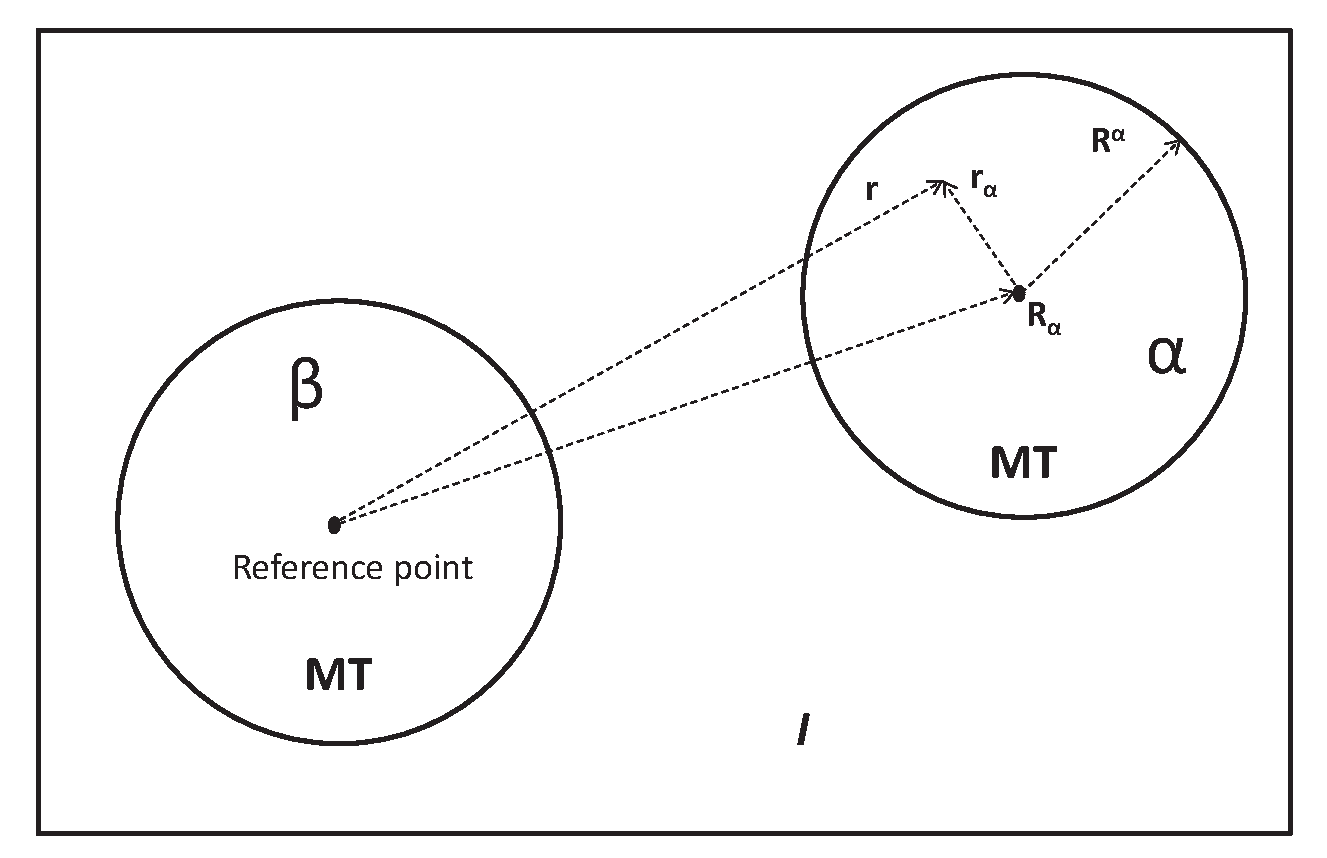
\includegraphics[scale=0.5]{unitcell.eps}
\caption{Partition of the unit cell.}
\label{ucuc}
\end{center}
\end{figure}

From \textbf{Fig. \ref{ucuc}}, one notices that unit cell is divided into MT spheres ($\alpha$, $\beta$) and an
(\textit{I}) region, where ${\textbf r = {\textbf R_{\alpha}}+{\textbf r_{\alpha}}}$ is guaranteed. The Rayleigh expansion formula yields

\begin{equation}
\expg<(\textbf {k}+\textbf{G})> = e^{i (\textbf {k}+\textbf{G}) \textbf{R}_{\alpha} } 4 \pi \sumlm<\ell><m> i^{\ell} \bessf< |\textbf{k}+\textbf{G}|> \sphfr<\ell{m}><r><> Y_{\ell{m}}(\widehat{\textbf{k}+\textbf{G}}).
\end{equation}
  
After matching those two representations, the following equation is satisfied for each ${\ell}m$

\begin{equation}
A _{{\ell}m}^{\alpha} (\textbf {k}+\textbf{G}) = \frac{ e^{i (\textbf {k}+\textbf{G}) \textbf{R}^{\alpha} } 4 \pi \sumlm<\ell><m> i^{\ell} \bessf< |\textbf{k}+\textbf{G}|> Y^{*}_{\ell{m}}(\widehat{\textbf{k}+\textbf{G}}) }{\sqrt{\Omega} u_{{\ell}}^{\alpha}(r_{\alpha}, E)}.
\end{equation}

The main drawbacks about the APW method is that the wavefuntion is energy dependent. It generates that
 the code needs to search for the energy in order to calculate the exact energy. Therefore it 
is really time-consuming. 

\subsubsection{Linearized augmented plane wave method}
\noindent In order to decouple the energy from the wavefunction, Andesen, Koelling and Arbman found out a way to seperate them, they noticed that the taylor expansion of the radial function
on certain energy, which can be given as

\begin{equation}\label{ap3}
 u_{{\ell}}(r_{\alpha}, E) = u_{{\ell}}(r_{\alpha}, E_{\ell}) + (E-E_{\ell}) \dot{u}_{{\ell}}(r_{\alpha}, E_{\ell}) + O((E-E_{\ell})^2).
\end{equation}

Therefore the basis fucntion is re-defined as 

\begin{equation}\label{lap4}
\phi^{LAPW}_{\textbf{k}+\textbf{G}} (\textbf{r}) = 
\begin{cases} \frac {1}{\sqrt{\Omega}} e^{i(\textbf{k}+\textbf{G})\textbf{r}} & \quad \mbox{if $\textbf{r} \in \textit{I} $}
\\
\sumg<\alpha>\sum\limits_{{\ell}m} f_{{\ell}{m}} (r_{\alpha},\textbf{k}+\textbf{G}, E_{\ell}) Y_{{\ell}m}(\hat{\textbf{r}}_{\alpha})  & \quad \mbox{if $r_{\alpha} \in MT. $}\\ 
\end{cases}
\end{equation}

Here, $f_{{\ell}{m}} (r_{\alpha},\textbf{k}+\textbf{G} ,E_{\ell}) =  A _{{\ell}m}^{\alpha} (\textbf {k}+\textbf{G}) u_{{\ell}}(r_{\alpha}, E_{\ell}) + B _{{\ell}m}^{\alpha} (\textbf {k}+\textbf{G}) \dot{u}_{{\ell}}(r_{\alpha}, E_{\ell})$
. $A _{{\ell}m}^{\alpha} (\textbf {k}+\textbf{G})$ and $B _{{\ell}m}^{\alpha} (\textbf {k}+\textbf{G})$ are the expansion coefficients, and $\dot{u}_{{\ell}}(r_{\alpha}, E_{\ell} )$ is the derivative of the radial function. Energy $E_{\ell}$  is considered as pre-calculated parameter in \textbf{Eq. \ref{lap4}}. Actually, it is chosen by the middle of  each $\ell$-character band, therefore this method is called linearized augmented plane wave (LAPW) method.

Apparently, LAPW method is more suitable in reality, because the wavefunction is decoupled with energy. However it has to match for two parameters.
Fortunately, it still take less time comparing with APW method. However, there is one drawback about this method, what if energy in the same $ {\ell} $ charater is different enough, 
which $E_{\ell}$ is correct? These states are called as semi-core states which exist in the actinides and the rare earths.

\subsubsection{Linearized augmented plane wave method plus local orbitals}
Comparing with LAPW method, linearized augmented plane wave method plus local orbitals (LAPW+LO) method extend and add smaller number of basis set, which is defined as


\begin{equation}\label{lap5}
\phi^{LO}_{\textbf{k}+\textbf{G}}(\textbf{r}) = 
\begin{cases} 0 & \quad \mbox{if $\textbf{r} \in \textit{I} $}
\\
(A _{{\ell}m}^{\alpha,LO}  u_{{\ell}}(r_{\alpha}, E_{\ell}) + B _{{\ell}m}^{\alpha,LO}  \dot{u}_{{\ell}}(r_{\alpha}, E_{\ell}) + C _{{\ell}m}^{\alpha,LO}  u_{{\ell}}(r_{\alpha}, E^{\prime}_{\ell})){Y_{{\ell}m}(\hat{\textbf{r}}_{\alpha})} & \quad \mbox{if $r_{\alpha} \in MT. $}\\ 
\end{cases}
\end{equation}
 

Here, $A _{{\ell}m}^{\alpha,LO}$, $B _{{\ell}m}^{\alpha,LO}$, and $C _{{\ell}m}^{\alpha,LO}$ can be obtained by normalization, as well as value and derivation on the sphere boundary to zero. The $E^{\prime}_{\ell}$ is
the chosen energy from semi-core state.

\subsubsection{Augmented plane wave method plus local orbitals}

There is one method which can solve the APW method efficiently, which is called as augmented plane wave method plus local orbitals (APW+lo). The 
basis function has two types: one is similar with APW method, but only without the derivative terms, that is, $f_{{\ell}{m}} (r_{\alpha},\textbf{k}+\textbf{G} ,E_{\ell}) =  A _{{\ell}m}^{\alpha}(\textbf{k}+\textbf{G})u_{{\ell}}(r_{\alpha}, E_{\ell})$; 
the other basis function is

\begin{equation}\label{lap6}
\phi^{lo}_\textbf{k+G} (\textbf{r}) = 
\begin{cases} 0 & \quad \mbox{if $\textbf{r} \in \textit{I} $}
\\
(A _{{\ell}m}^{\alpha,lo}  u_{{\ell}}(r_{\alpha}, E_{\ell}) + B _{{\ell}m}^{\alpha,lo}  \dot{u}_{{\ell}}(r_{\alpha}, E_{\ell}) ){Y_{{\ell}m}(\hat{\textbf{r}}_{\alpha})} & \quad \mbox{if $r_{\alpha} \in MT. $}\\ 
\end{cases}
\end{equation}
 
The value of $A _{{\ell}m}^{\alpha,lo}$ and $B _{{\ell}m}^{\alpha,lo}$ are obtained by normalization and local orbital has zero value at the muffin tin boundary. This method can not solve semicore states like LAPW+LO.
However, it does increase the efficiency to linearize Slater's APW method. Certainly, it exsits some types of basis function which can mix the advantages from mentioned methods.

\subsection{Effective potential}

\label{epote}
The potential in the FPLAPW method is also divided into two regions, the MT region and the \textit{I} region.
\begin{equation*}\label{lap7}
V(\textbf{r}) = 
\begin{cases} \sumg<{\textbf G}> V_{\textbf G} e^{i {\textbf G} {\textbf {r}  }} & \quad \mbox{if $\textbf{r} \in \textit{I} $}
\\
 \sum\limits_{{\ell}m} V_{{\ell}m}^{\alpha} (r_{\alpha}) Y_{{\ell}m}(\hat{{\textbf r}}_{\alpha})  & \quad \mbox{if $r_{\alpha} \in MT. $}\\ 
\end{cases}
\end{equation*}

\section{Dielectric function}
The dielectric function describes the optical property of materials. Normally, it is written as $\varepsilon$, which has two parts

\begin{equation}
 \varepsilon = \varepsilon_1 + i \varepsilon_2.
\end{equation}

Here, $\varepsilon_1$ denotes how much the material is polarized when an electric field is applied, and $\varepsilon_2$ is related with absorption of the material. The imaginary part of interband contribution to the dielectric function is defined as

\begin{equation}\label{df2}
\varepsilon_2^{\alpha\beta} = \frac{\hbar e^2}{\pi m^2\omega^2} \sum_{cv} \int d \textbf {k} <\Psi_{c{\textbf k}}|p^\alpha|\Psi_{v{\textbf k}}><\Psi_{v{\textbf k}}|p^\beta|\Psi_{c{\textbf k}}> (f(\varepsilon_{c \textbf k})-f(\varepsilon_{v \textbf k}))\delta(\varepsilon_{c {\textbf k}}-\varepsilon_{c{\textbf k}}-\omega).
\end{equation}

Here, $c$ and $v$ are the index of conduction band and valence band, respectively. The total imaginary part of dielectric function can be calculated when $c$ and $v$ run over all the conduction bands and valence bands. Similarily, the
interband contribution can be achived by calculating single conduction band and single valence band.   

The real part of dielectric function can be calculated by Kramers-Kronig relations

\begin{equation}
 \varepsilon_1^{\alpha\beta} = \delta^{\alpha\beta}+\frac{2}{\pi}P\int^{\infty}_{0} \frac{\omega'\varepsilon_2^{\alpha\beta}(\omega')}{\omega'^{2}-\omega^{2}} d\omega'.
\end{equation}


The absorption coefficient can be obtained by the real part and imaginary part of dielectric function
\begin{equation}
 \alpha(\omega) = \frac{\sqrt{2}\omega}{c} \left[ \sqrt{{\varepsilon_1(\omega)}^2+{\varepsilon_2(\omega)}^2}-{\varepsilon_1(\omega)} \right]^{1/2}.
\end{equation}

In this section, only some basic equations are covered when it is related to calculate the dielectric function. If someone is interested in this topic, one can find more detailed in Ref. $??$.

\begin{comment}
\section{k $\cdot$ p method}
\label{kpmaa}

The band dispersion can be obtained exactly by using the $\bold k \cdot \bold p$ method in principle, the basic idea will be explained in the following text.

First, if the Schrödinger equation is defined as follows:

\begin{equation}\label{kpse}
\left\{ \frac {{\textbf p}^2} {2m} + V({\textbf r}) \right\} \wfbloch<n>< \bold k> = \ebloch<n><\bold k> \wfbloch<n><\bold k>,
\end{equation}

where ${\textbf p} = i \hbar \bigtriangledown $, and the Bloch theory shows:

\begin{equation}\label{1}
 \wfbloch<n><\bold k> = \expg<k> \ubloch<n><\bold k>,
\end{equation}

where $\wfbloch<n><\bold k>$ is the wavefunction on ${\textbf k}$ point for the {$\textit n$}th band, and $\expg<k>$ is plane wave, $\ubloch<n><\bold k>$ is a function which has the same a periodicity as the potential.

If substituting the Eq. \ref{1} to Eq. \ref{kpse}, it will end up the following equation:

\begin{equation}
 \{  \frac{{\textbf p}^2}{2m} + V({\textbf r }) + \frac{{\hbar^2 {\textbf k}^2}}{2m} + \frac{{\hbar \textbf {kp}}}{m} \} \ubloch<n><\bold  k>  =  \ebloch<n><\bold  k> \ubloch<n><\bold  k>.
\end{equation}

In the above equation, if $\textbf k = \textbf 0$, then the Hamiltonian turn out to be $H_0 = {\textbf p}^2 / {2m} + V({\textbf r })$. Here the first two terms are treated as unpertubation term, and pertubation term is seen as
$W={{\hbar^2 {\textbf k}^2}}/{2m} + {{\hbar \textbf {kp}}}/{m}$, the result will be as follows after treating the equation as pertubation.

\begin{equation}
 \ebloch<n><\bold k> = E_{n,\textbf 0} + \frac{{\hbar^2 {\textbf k}^2}}{2m} + \frac{ \hbar^2}{m^2} \suminj<i><j> \frac{|<\ubloch<n><\bold 0>|{\textbf {kp}}|\ubloch<n'><\bold  0>>|^2}{E_{n,\textbf 0} - E_{n',\textbf 0}}.
\end{equation}


Now let us suppose the wavefunction and energy are obtained by some procedures on $\bold k_0$ point, $\wfbloch<n><\bold  k_0>$ is the wavefunction and $\ebloch<n><\textbf  k_0>$ is the energy.
Another function is defined as follows:

\begin{equation}\label{2}
\chikp<n><\textbf k> = \expg<(\bold k-\bold {k_0})>  \wfbloch<n><\bold {k_0}>.
\end{equation}

The above function $\chikp<n><\textbf k> $ is expanded as wavefunction on ${ \textbf k}$ point, and then the wavefunction on the ${\textbf k}$ point is calculated by:
\begin{equation}\label{3}
\wfbloch<n><\bold k> =  {\sum\limits_{j}} C_{n,j}^{\bold k} \chikp<j><\bold k>. 
\end{equation}

From above equation, the wavefunction is known if the coefficient $C_{n,j}^{\bold k}$ is obtained, let us substitute the Eq. \ref{3} into Kohn-Sham Eq. \ref{kpse}.
Finally the following equation is obtained:

\begin{equation}\label{5}
{\sum\limits_{j}}  C_{n,j}^{\bold k} \left \{  \left [  \ebloch<j><\bold {k_0}> -  \ebloch<n><\bold k>  + \frac{{\hbar}^2}{2m} { (\bold {k}^2- \bold {k}_0^2)}    \right ] \delta_{j',j} + \frac{\hbar}{m} {(\bold {k}-\bold{k}_0)} {\overline{\textbf{p}}_{j',j}} \right \} = 0,
\end{equation}

where ${\overline{\textbf{p}}_{j',j}} = \langle \ubloch<j'><\bold {k_0}>| {\textbf p} | \ubloch<j><\bold {k_0}>  \rangle $.
 
We also can simpify the above equation in the following format:
\begin{equation}\label{6}
{\sum\limits_{j}} C_{n,j}^{\bold {k}} \left \{ H_{j',j}- \ebloch<n><\bold {k}> \delta_{j',j} \right \} =0,
\end{equation}

where
\begin{equation} \label{7}
H_{j',j} = \left [  \ebloch<j><\bold {k_0}>  + \frac{{\hbar}^2}{2m} { (\bold{k}^2-\bold{k}_0^2)}    \right ] \delta_{j',j} + \frac{\hbar}{m} {(\bold{k}-\bold{k}_0)} {\overline{\textbf{p}}_{j',j}}.
\end{equation}

From the above equation, the coefficient $ C_{n,j}^{\bold k}$ and $\ebloch<n><\bold {k}>$ are calculated.
\end{comment}

\section{Spin-orbit coupling}
\label{srasoc}

\subsection{Dirac equation}

Non-relativistic quantum mechanics has broad application. However the non-relativistic quantum is not suitable to describe the system where the speed of electron is near the speed of light $c$. 
Therefore, Dirac introduced an equation which is called Dirac equation applying for relativistic case.

\noindent Dirac defined the Hamiltonian as

\begin{equation}\label{dirac}
{H}_\textit{dirac} = c \boldsymbol{\alpha} \textbf{P} + \boldsymbol{\beta}mc^{2} + V.
\end{equation}

\noindent Here, $\textbf{P} = -i\hbar \nabla $ is the momentum operator, $V$ is the general potential, and $m$ is the mass of electron. 
 $\boldsymbol{\alpha}$ and $\boldsymbol{\beta}$ are $4 \times 4$ matrices, which are defined as
\begin{equation}
 \boldsymbol{\alpha} = \left( \begin{array}{cc}
 0 & \boldsymbol{\sigma}  \\
 \boldsymbol{\sigma} & 0   \end{array} \right),
\boldsymbol{\beta} = \left( \begin{array}{ccc}
\boldsymbol{I} & 0\\
0 & -\boldsymbol{I}\end{array} \right).
\end{equation}

\noindent Here, $\boldsymbol{I}$ is unit matrix. $\boldsymbol{\sigma}$ is Pauli matrix, which is given as

\begin{equation} 
\boldsymbol{\sigma} = (\boldsymbol{\sigma}_x \  \boldsymbol{\sigma}_y \  \boldsymbol{\sigma}_z )  
\end{equation}

\begin{equation}
\boldsymbol{\sigma}_x = \left( \begin{array}{cc}
0 & 1\\
1 & 0\end{array} \right),
\boldsymbol{\sigma}_y = \left( \begin{array}{ccc}
0 & -i\\
i & 0\end{array} \right),
\boldsymbol{\sigma}_z = \left( \begin{array}{ccc}
1 & 0\\
0 & -1\end{array} \right).
\end{equation}

\subsection{Derivation of spin-orbit coupling}

\noindent  Assume that $\Psi$ is the wavefunction of Hamiltonian in \textbf {Eq. \ref{dirac}} which has four components. However, it can be 
written with only two terms
\begin{equation}\label{diracwf}
\Psi = \left( \begin{array}{c}
\phi^{\uparrow} \\
\phi^{\downarrow} \\
\chi^{\uparrow} \\
\chi^{\downarrow} \end{array} \right),
 \Psi = \left(\begin{array}{c}
\phi \\               
\chi \end{array} \right).
\end{equation}

\noindent Here, $\phi$ includes the two terms of $\phi^{\uparrow}$ and $\phi^{\downarrow}$, and $\chi$ contains  $\chi^{\uparrow}$ and $\chi^{\downarrow}$.
Under the nonrelativistic limit, $\phi$ is bigger than $\chi$ by the ratio of $v/c$. Here, $v$ and $c$ are speed of particle and light, respectively.
Therefore, the $\phi$ is considered as the large term and $\chi$ is the small one.

\noindent In order to derive the spin-orbit coupling term, we need to take use of the nonrelativistic limit approximation ($v^2/c^2 << 1$). The time-independent Dirac equation is give as

\begin{equation}\label{diracse}
 E \Psi = (c \boldsymbol{\alpha} \textbf{P} + \boldsymbol{\beta}mc^{2} + V) \Psi.
\end{equation}

\noindent For convenience, the following equation is defined

\begin{equation}\label{dirace}
E^{\prime} = E - mc^2.
\end{equation}

\noindent Here, $E$ is the total energy, $mc^2$ and $E'$ are the rest mass energy and the remaining energy excluding the rest mass energy, respectively. Under the nonrelativistic limit, 
$E'$ is far smaller than $mc^2$. The following equation is given when \textbf{Eq. \ref{diracwf}} and \textbf{Eq. \ref{dirace}} are put into \textbf{Eq. \ref{diracse}}

\begin{equation}
\begin{split}
&(E^{\prime} - V) \Phi - c \boldsymbol{\sigma} \textbf{P} \chi = 0\\                
&-c\boldsymbol{\sigma} \textbf{P} \Phi + (E^{\prime}+2mc^2-V)\chi = 0.
\end{split}
\end{equation}

\noindent To eliminate the $\chi$ (otherwise, it is the antiparticle problem), it ends up with the equation
  \begin{equation}
(V + \frac{1}{2m} (\boldsymbol{\sigma} \textbf{P}) (1+\frac{E^{\prime}-V}{2mc^2})^{-1} (\boldsymbol{\sigma} \textbf{P}) )\phi=E^{\prime}\phi,
\end{equation}

\noindent where ${E^{\prime}-V}$ is far smaller than ${2mc^2}$, therefore taking advantage of the taylor expansion of it,  as well as the following identites
\begin{equation}
\begin{split}
& [\textbf{P}, V ] = -i \hbar \triangledown V \\                
&(\boldsymbol{\sigma} \textbf{A} )(\boldsymbol{\sigma} \textbf{B}) = \textbf{A} \textbf{B} + i\boldsymbol{\sigma}[\textbf{A} \times \textbf{B}].
\end{split}
\end{equation}

The final equation is obtained under the nonrelativistic limit

\begin{equation}
E^{\prime} \phi = (\frac{\textbf{P}^2}{2m} + V - \frac{\textbf{P}^4}{8 {m}^3 {c}^2}-\frac{i\hbar}{4{m}^2 {c}^2} (\nabla{V})\textbf{P}+\frac{\hbar}{4 m^2 c^2} \boldsymbol{\sigma}[\nabla{V} \times \textbf{P}]) \phi.
\end{equation}

Furthermore, we can approximate the above equation to the simpler expression under spherical symmetry potential

\begin{equation}
 E^{\prime} \phi = (\frac{\textbf{P}^2}{2m} +V - \frac{\textbf{P}^4}{8 {m}^3 {c}^2}-\frac{i\hbar}{4{m}^2 {c}^2} (\nabla{V})\textbf{P}+\frac{1}{2 m^2 c^2} \frac{1}{R} \frac{dV}{dR}\textbf{S}\textbf{L}) \phi.
\end{equation}

\noindent Here, $\textbf{S} = {\hbar}{\boldsymbol{\sigma}}/2$ is the Pauli spinor, and $\textbf{L} = \textbf{R} \times \textbf{P}$ is the orbital
angular momentum operator. The terms of ${\textbf{P}^2}/(2m) + V$ is Schrödinger term,  ${\textbf{P}^4}/(8 {m}^3 {c}^2)$ and ${i\hbar} (\nabla{V})\textbf{P} /(4{m}^2 {c}^2)$  are the mass enhancement 
and Darwin term, respectively, both of them together is called the scalar relativistic approximation (SRA). The last term is the spin-orbit coupling (SOC) term. One has to
notice that the Darwin term is not hermitian operator, alternatively, $\nabla^2{V} /(8{m}^2 {c}^2)$ is suggested in the realistic implementation.


\chapter{Results and discussion}

In this section, the major results for the licentiate thesis are demonstrated. The first one is parameterization of energy bands for CuIn{\textsubscript{1-x}}Ga{\textsubscript{x}}Se\textsubscript{2} (CIGS) 
where $x$ = 0, 0.5, and 1, as well as indirect results based on the parameterization. The second one is the calculation of the dielectric function spectra for the CuIn{\textsubscript{0.5}}Ga{\textsubscript{0.5}}Se\textsubscript{2} by
all electron and full-potential linearized augemented plane wave (FPLAPW) method, which is compared with experimental results as well. While the probable electronic orginins of the critical point (CP) features are discussed.

\section{Parameterization of energy bands for CIGS}

\subsection{Parameterization method}
The curvature of energy bands is often demonstrated by the effective electron and hole masses, therefore the parabolic energy dispersion of energy bands, also named parabolic band approximation (pba), is given as

\begin{equation}\begin{split}\label{parabolic}
& E_{j}^{pb}(\textbf{k}) = E_{j}(\textbf{0}) \pm \left[ \frac{\widetilde{\textbf{k}}_{x}^{2}+\widetilde{ \textbf{k}}_{y}^{2}}{m_{j}^{\perp}} + \frac{\widetilde{\textbf{k}}_{z}^{2}}{m_{j}^{\parallel}} \right] \\
& \widetilde{\textbf{k}}_{\alpha}^{2} = \frac{\hbar {\textbf{k}}_{\alpha}^{2}}{2e}, \textrm{where}\  \alpha = x, y, \textrm{and}\  z.
\end{split}
\end{equation}

Here, $m_{j}^{\perp}$ and $m_{j}^{\parallel}$ are transverse electron masses and longitudinal electron masses, respectively.

\begin{table}[H]
\centering
 \captionsetup{width=1\textwidth}
\scalebox{0.9}{
 \begin{tabular}{c l l l l l l l l l l l l }
\hline
 &\multicolumn{4}{c}{CuInSe\textsubscript{2}}&\multicolumn{4}{c}{CuIn\textsubscript{0.5}Ga\textsubscript{0.5}Se\textsubscript{2}}&\multicolumn{4}{c}{CuGaSe\textsubscript{2}}\\
\cline{2-13}
 Parameters & c1 & v1 & v2 & v3 & c1 & v1 & v2 & v3 & c1 & v1 & v2 & v3\\
\hline\hline
$E_j(\textbf{0})$ &0.97	 &0	&0.01	&0.19	&1.2	&0	&0.02	&0.2	&1.47	&0	&0.08	&0.26\\
$m_j^{\bot}$      &0.08	 &0.14	&0.25	&0.27	&0.1	&0.4	&0.17	&0.29	&0.13	&0.47	&0.2	&0.29 \\
$m_j^{||}$        &0.09  &0.66	&0.12	&0.28	&0.11	&0.14	&0.61	&0.4	&0.13	&0.15	&0.61	&0.49 \\
\hline
\end{tabular}}
\caption {Parameters of \textbf{Eq. \ref{parabolic}} to describe the parabolic energy dispersions of the lowest conduction band (CB) and the three uppermost valence bands (VBs) in the vicinity of the $\Gamma$-point. $E_{v1}(\textbf{0})$ is the valence band maximum (VBM) and 
$E_{c1}(\textbf{0})$ is the fundamental band-gap energy Eg.}\label{pm1}
\end{table}

 
Unfortunately, these effective masses are only valid around the considered {\textbf k} point, which is not suitable to describe the non-parabolic away from this {\textbf k} point. However, the accurate shape of energy bands is 
important when one simulates and analyzes the electron transport or band filling for some materials.

In this work, we have parameterized the three uppermost VBs and the lowest CB for the materials $\cigs$ where $x$ = 0, 0.5, and 1, that is, $\mathrm{CuInSe_2}$, $\mathrm{CuIn_{0.5}Ga_{0.5}Se_2}$, and $\mathrm{CuGaSe_2}$. This 
parameterization is based on the all electron and full-potential linearized augemented plane wave (FPLAPW) calculation. Normally, the \textbf{k $\cdot$ p} method is utilized to parameterize the energy bands. However, the energy
dispersions of $\cigs$ are rather complex due to the crystal-field interaction and the spin-orbit coupling. Therefore, the regular \textbf{k $\cdot$ p} method is not sufficient to describe the energy bands. We manage to extend the
\textbf{k $\cdot$ p} expression to higher orders, which is called full band parameterization (fbp) in the following text. Thb fbp is valid around 0.5 eV below VBM and 0.5 eV above conduction band minimum (CBM). The explicit equation 
is given as

\begin{equation}\label{nonparabolic}
\begin{split}
& \small E_j(\textbf{k}) = E_{j}^{pb}(\textbf{k}) + E_j^0 + \Delta_{j,1} \left( \delta_{j,1}^2 \left( \frac{\widetilde{\textbf{k}}_{x}^{4}+\widetilde{ \textbf{k}}_{y}^{4}}{m_{0}^{2}} \right) + \delta_{j,2}^2 \left( \frac{\widetilde{\textbf{k}}_{x}^{2}\widetilde{\textbf{k}}_{y}^{2}}{m_{0}^2} \right) + 1 \right)^{1/2} \\
& \small + \Delta_{j,2} \left( \delta_{j,3}^3 \left( \frac{\widetilde{\textbf{k}}_{x}^{6}+\widetilde{ \textbf{k}}_{y}^{6}}{m_{0}^{3}} \right) + \delta_{j,4}^3 \left( \frac{\widetilde{\textbf{k}}_{x}^{2}\widetilde{\textbf{k}}_{y}^{4} + \widetilde{\textbf{k}}_{x}^{4}\widetilde{\textbf{k}}_{y}^{2}}{m_{0}^3} \right) + 1 \right)^{1/3} \\
& \small + \Delta_{j,3} \left( \delta_{j,5}^2 \left( \frac{\widetilde{\textbf{k}}_{z}^{4}}{m_0^2} \right) + 1 \right)^{1/2} + \Delta_{j,4} \left( \delta_{j,6}^3 \left( \frac{\widetilde{\textbf{k}}_{z}^{6}}{m_0^3} \right) + 1 \right)^{1/3} \\
& \small + \Delta_{j,5} \left( \delta_{j,7}^2 \left( \frac{\widetilde{\textbf{k}}_{x}^{2}\widetilde{\textbf{k}}_{z}^{2} + \widetilde{\textbf{k}}_{y}^{2}\widetilde{\textbf{k}}_{z}^{2}}{m_{0}^3} \right) + 1 \right)^{1/2} \\
& \small + \Delta_{j,6} \left( \delta_{j,8}^3 \left( \frac{\widetilde{\textbf{k}}_{x}^{4}\widetilde{\textbf{k}}_{z}^{2} + \widetilde{\textbf{k}}_{y}^{4}\widetilde{\textbf{k}}_{z}^{2}}{m_{0}^3} \right) + \delta_{j,9}^3 \left( \frac{\widetilde{\textbf{k}}_{x}^{2}\widetilde{\textbf{k}}_{z}^{4} + \widetilde{\textbf{k}}_{y}^{2}\widetilde{\textbf{k}}_{z}^{4}}{m_{0}^3} \right) + \delta_{j,10}^3 \left( \frac{\widetilde{\textbf{k}}_{x}^{2}\widetilde{\textbf{k}}_{y}^{2}\widetilde{\textbf{k}}_{z}^{2}}{m_{0}^3} \right) +1 \right)^{1/3}.
\end{split}\end{equation}

Here,  $E_j^0$, $\Delta_{j,n}$, and $\delta_{j,m}$ are fitting parameters (\textbf{Table. \ref{nonpara}}), ${m_0}$ is the electron rest mass. In the \textbf{Eq. \ref{nonparabolic}}, each term represents one parabolic dispersion, the
higher order terms describe the larger wave vectors away from $\Gamma$ point. Unfortunately, the complex energy dispersions of $\cigs$ requires many fitting parameters. However, the conduction band need less fitting parameters.


 \begin{sidewaystable}
 \captionsetup{width=1\textwidth}
\scalebox{0.9}{
 \begin{tabular}{c l l l l l l l l l l l l }
\hline
 &\multicolumn{4}{c}{CuInSe\textsubscript{2}}&\multicolumn{4}{c}{CuIn\textsubscript{0.5}Ga\textsubscript{0.5}Se\textsubscript{2}}&\multicolumn{4}{c}{CuGaSe\textsubscript{2}}\\
\cline{2-13}
 Parameters & c1 & v1 & v2 & v3 & c1 & v1 & v2 & v3 & c1 & v1 & v2 & v3\\
\hline\hline
$E_j^0$                &$-$4.010&$-$5.311&$-$5.242&$-$5.620&$-$4.146&$-$6.210&$-$6.426&$-$5.835&$-$3.927&5.284    &$-$5.789&$-$2.783\\
$\bigtriangleup_{j,1}$ &$-$0.295&0.006	 &$-$0.002&$-$0.021&$-$0.230&	0.106&	 1.321&$-$0.026&$-$0.454&0.116    &   1.284&$-$1.194 \\
$\bigtriangleup_{j,2}$ &    0	&0.098	 &   0.104&   0.308&   0    &   0.002&   0.096&	  0.386&0       &$-$10.771&$-$0.837&$-$0.024 \\
$\bigtriangleup_{j,3}$ &$-$0.242&0.018	 &0.124   &$-$0.025&$-$0.293&	0.937&$-$0.017&$-$0.838&$-$0.419&0.088    &0.347   &$-$0.303 \\
$\bigtriangleup_{j,4}$ & 0      &0.188   &0.076	  &   0.238&  0     &   0.021&   0.163&0.789   &0	&0.076    &$-$0.051&   0.608 \\
$\bigtriangleup_{j,5}$ &$-$0.016&$-$0.048&0.001   &$-$0.009&$-$0.046&   0.001&	 0.011&	0.37   &$-$0.047&0.022    &0.274   &   0.374 \\
$\bigtriangleup_{j,6}$ & 0	&0.037   &$-$0.073&   0.117&	0   &$-$0.022&$-$0.313&$-$0.012&0       &$-$0.111 &$-$0.525&$-$4.362 \\
$\delta_{j,1}$         & 30.669	&952     &2304.147&  94.139&  27.157&	5.517& 1.029  &  57.007&  11.865&10.526   &9.269   &   3.839 \\
$\delta_{j,2}$         & 47.374	&1754.386&4587.156& 220.556&  44.506&	13.61&0.413   &153.435 &  20.262&28.545   &21.582  &   6.232 \\
$\delta_{j,3}$         & 0	&3.97    &72.296  &11.746  &0	    &487.805 &46.95   &8.489   &0	&0.131    &9.116   &  59.625 \\
$\delta_{j,4}$         & 0	&3.688	 &123.274 &18.078  &0	    &1128.668&72.844  &13.509  &0	&0.126	  &21.328  & 148.516 \\
$\delta_{j,5}$         & 31.852	&6.041	 &56.004  &64.137  &21.124  &1.314   &247.158 &7.921   &12.978	&7.709	  &12.141  &   8.014 \\
$\delta_{j,6}$         & 0	&3.134	 &6.1	  &12.031  & 0	    &267.523 &29.076  &8.743   &0	&64.185	  &66.808  &   5.309 \\
$\delta_{j,7}$         & 222.641&37.004	 &3846.154&206.148 &79.879  &3322.259&212.902 &16.836  &76.319  &236.742  &16.24   &   5.092 \\
$\delta_{j,8}$         & 0	&12.647	 &16.269  &6.982   &0	    &92.954  &4.885   &57.89   &0	&31.947	  &6.71	   &   1.209 \\
$\delta_{j,9}$         & 0	&61.565	 &33.169  &34.114  &0	    &118.064 &0	      &273.4   &0       &34.784   &4.831   &   1.394 \\
$\delta_{j,10}$        & 0	&46.679	 &31.275  &32.237  &0	    &110.327 &6.074   &153.523 &0	&40.765	  &5.243   &   2.124 \\
\hline
\end{tabular}}
\caption {Parameters of \textbf{Eq. \ref{nonparabolic}} to describe the non-parabolic contribution to the energy dispersions $E\textsubscript{j}(\textbf{k})$ of the lowest CB and the three uppermost VBs. The notation of the energy 
bands ($j$ = $c1$, $v1$, $v2$, and $v3$) refers to a spin-independent band indexing, where $c1$ represents the bottommost CB and $v1$ represents the topmost valence band (VB) (see \textbf{Fig. \ref{bandstruct}}.}\label{nonpara}
\end{sidewaystable}


\subsection{Non-parabolicity properties}

The fbp of $\cigs$ ($x$ = 0, 0.5, and 1) are plotted compared with the calculation based on the FPLAPW method and the pba in \textbf{Eq. \ref{parabolic}}.

\begin{figure}[H]
    \begin{center}
            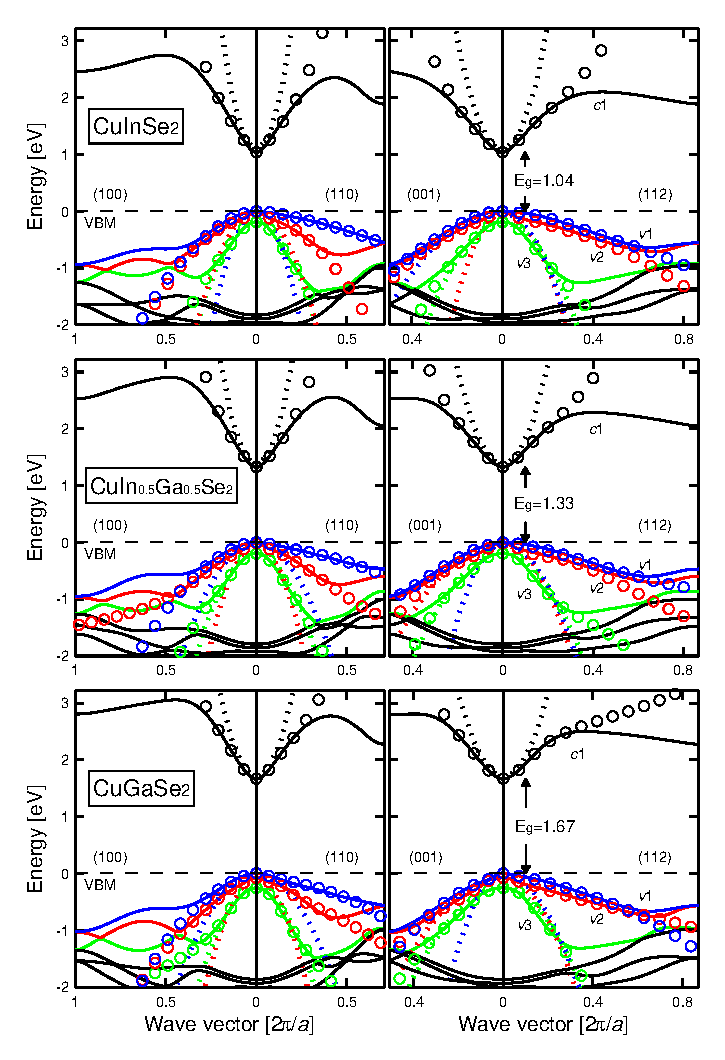
\includegraphics[width=0.45\textwidth,clip]{paper2figure1}
            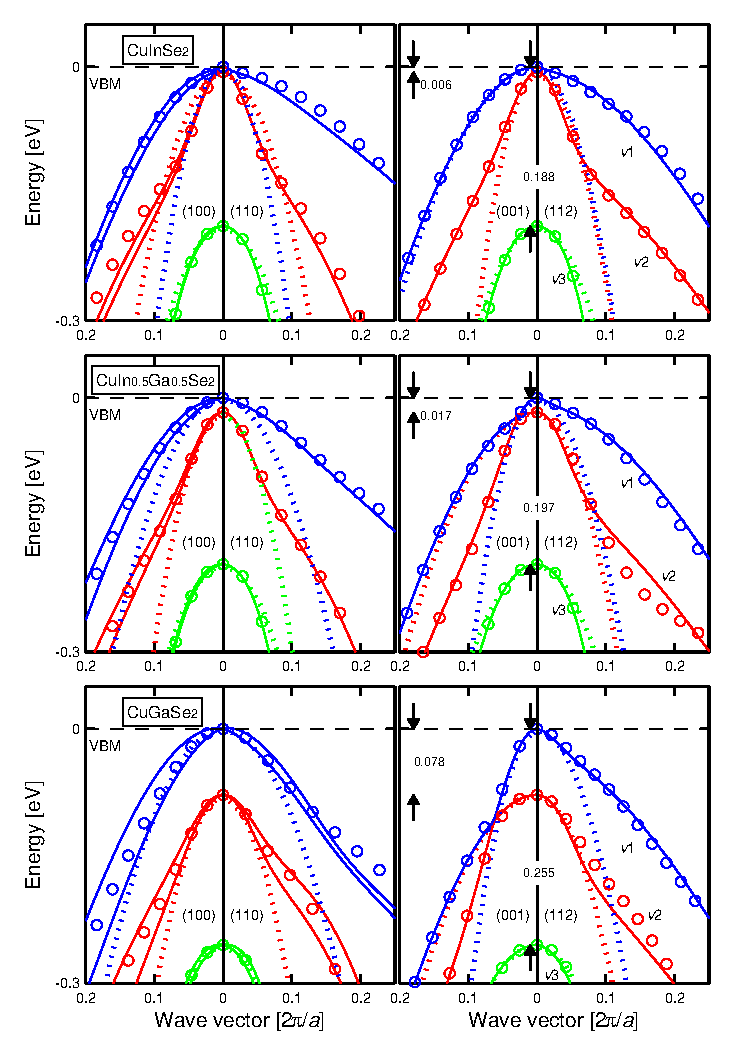
\includegraphics[width=0.46\textwidth,clip]{paper2figure2}
     \end{center}
    \caption{ Left panel: Electronic band structure along four directions. The circles are the results of the full band parameterization (fbp), and the dotted lines represent the parabolic band approximation (pba). Righ panel: The 
              close-up of left panel for the valence bands close to $\Gamma$ point.}      
    \label{bandstruct}
\end{figure}

From \textbf{Fig. \ref{bandstruct}}, one will observe that the parameterized energy bands can describe the energy below VBM around 0.5 eV accurately, and around 0.5 eV above the CB minimum (CBM) as well. However, the pba is only
valid below VBM around $-$4, $-$10, and $-$40 meV for $\mathrm{CuInSe_2}$, $\mathrm{CuIn_{0.5}Ga_{0.5}Se_2}$, and $\mathrm{CuGaSe_2}$, respectively. Since the lowest conduction band is more parabolic, therefore, the less fitting 
parameters are expected (\textbf{Table \ref{nonpara}}).

To further ultilize this parameterization method, the energy dispersions of the lowest CB and the three uppermost VBs are parameterized for Kesterite and Stannite Cu\textsubscript{2}ZnSn(S,Se)\textsubscript{4} as well. It works as 
good as CIGS, therefore, this parameterization method can be ultilized to other materials potentially.

\begin{figure}[H]
    \begin{center}
            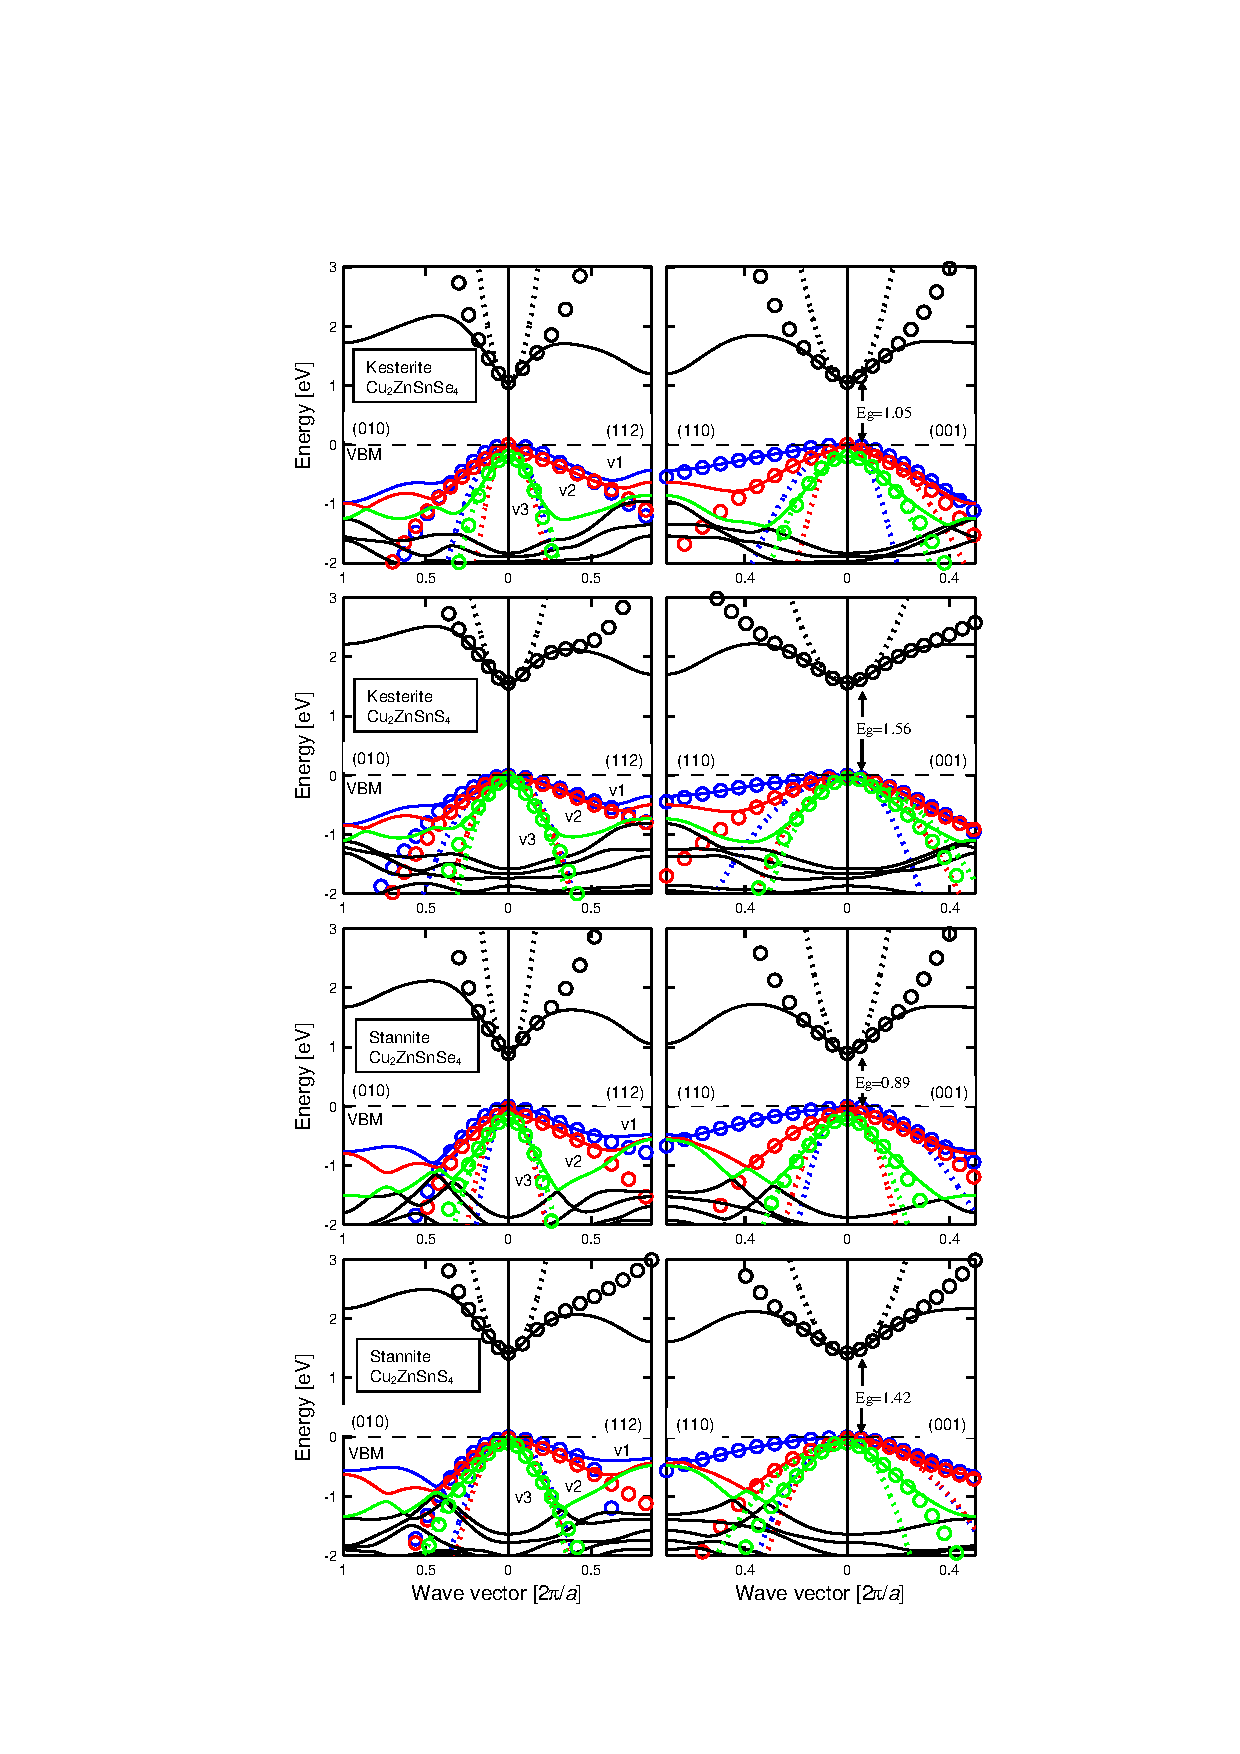
\includegraphics[width=1\textwidth,clip]{bandstr}
     \end{center}
    \caption{ Electronic band structure of the kesterite and stannite structures of Cu\textsubscript{2}ZnSnS\textsubscript{4} and Cu\textsubscript{2}ZnSnSe\textsubscript{4} along the symmetry directions (kx, ky, kz) = (010), (112),
              (110), and (001). The circles are the results of the full band parameterization (fbp), and the dotted lines represent the parabolic band approximation (pba). }      
    \label{bandstruct1}
\end{figure}


In order to demonstrate the anisotropic and non-parabolic of energy bands further, the constant energy surface $S_j(E)$ is determined for CuInSe\textsubscript{2} and CuGaSe\textsubscript{2}.

\begin{figure}[H]
    \begin{center}
            \includegraphics[width=0.46\textwidth,clip]{fermi_sphere_cii}
           % \includegraphics[width=0.4\textwidth,clip]{fermi_sphere_cig}
            \includegraphics[width=0.4\textwidth,clip]{fermi_sphere_cgg}
     \end{center}
    \caption{Constant energy surfaces for the three uppermost VBs and the lowest CB for the energies E = 1 meV (left column ellipsoidal) and E = 200 meV (right column).  
The CuInSe\textsubscript{2} and CuGaSe\textsubscript{2} are demonstrated in this figure.}
    \label{cse}
\end{figure}

In the \textbf{Fig. \ref{cse}}, 1 meV represents that it is near to $\Gamma$ point ; 200 meV implies that it is far away the $\Gamma$ point.
One will notice that the pba is proper to describe the energy bands close to the $\Gamma$ point, and it is ellipsoidal shaped sphere. For example,
for the topmost VB ($v_1$) of $\mathrm{CuInSe_2}$, the constant energy surface is ellipsoidal in the vicinity of the $\Gamma$ point since the effective
masses are anisotropic ($m_{v1}^{\perp}$ = 0.14$m_0$ and $m_{v1}^{\parallel}$ = 0.66$m_0$ in \textbf{Table \ref{pm1}}). However, the constant energy surface becomes non-ellipsoidal when the energies 
is far away from $\Gamma$ point. For example, for the same band, the constant energy surface is not ellipoidal shape at all when the energies goes up to 200 meV. It also implies that it is not correct to consider the constant 
effective mass for simulation. For the CB, the change is relatively small.

\subsection{Application of the full band parameterization}

The parameterized energy bands can be exploited to reveal the detailed information near the VB and CB edged. In this section, the effective masses, density-of-states (DOS), .... are caluclated based on
this fbp. In comparison with the results based on pba, most of the results are calculated with the pba as well.  

The effective masses are \textbf{k}-independent for the pba, which is not fully correct due to the non-parabolicity and anisotropy of the energy bands.  The effective masses tensors are calculated numerically by

\begin{equation}\label{inversemasse}
m_j(\textbf{k}) = \pm \hbar^2/(\partial^2 E_j(\textbf{k})/\partial\textbf{k}^2) \ \textrm{where}\  j = c1, v1, v2, \textrm{and}\  v3.
\end{equation}

The result from \textbf{Fig. \ref{inversemessf}} demonstrates that the energy bands of $\cigs$ are strong non-parabolic, since it should be constant in the pba along each symmetry direction. The effective hole masses of the two 
topmost VBs are very anisotropy close to the $\Gamma$ point, however, the electron masses of conduction bands are rather isotropic ($m_{c1}^{100}(\textbf{0}) \approx m_{c1}^{110}(\textbf{0}) \approx m_{c1}^{001}(\textbf{0}) 
\approx m_{c1}^{112}(\textbf{0})$). Hole masses of CuGaSe\textsubscript{2} vary somewhat less compared with those of CuInSe\textsubscript{2} due to CuGaSe\textsubscript{2} has larger split between the VBs. In order to better 
visibility, therefore, the inverse of the mass are presented.

\begin{figure}[H]
    \begin{center}
            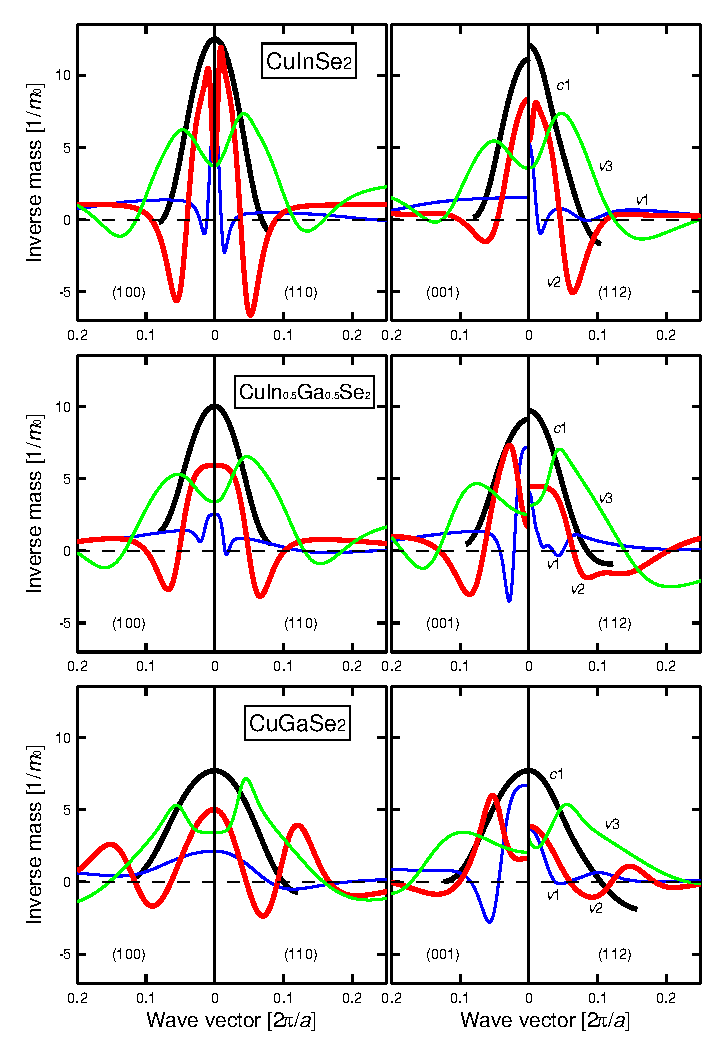
\includegraphics[width=0.43\textwidth,clip]{paper1figure3}
     \end{center}
    \caption{ Inverse of the effective electron and hole masses in the four symmetry directions for the $\cigs$ (x=0, 0.5, and 1).}      
    \label{inversemessf}
\end{figure}

In order to further analyze the impact of non-parabolicity and anisotropy of the energy bands, the density-of-states (DOS) is calculated based on fba and pba. The DOS in $j$th band is defined as

\begin{equation}\label{dosj}
 g_j(E)=\frac{1}{\Omega} \sum \limits_{\textbf{k}} 2 \delta (E-E_j(\textbf{k})) = \frac{1}{4\pi^3} \int \limits_{E_j(\textbf{k}) = E} \frac{dS(\textbf{k})}{|\bigtriangledown_\textbf{k} E_j(\textbf{k})|}.
\end{equation}
 
Here, $E_j(\textbf{k}) = E$ is the $\textbf{k}$ space surface with constant energy $E$, and the $\bigtriangledown_\textbf{k} E_j(\textbf{k})$ is the gradient of the energy dispersion.
In the case of the pba, the \textbf{Eq. \ref{dosj}} can be written as

\begin{equation}\label{dosjp}
 g_j^{pba}(E) = \frac{1}{2\pi^2} \big(\frac{2m_j^{DOS}}{\hbar^2}\big)^{3/2} \sqrt{|E-E_j(\textbf{0})|}.
\end{equation}
 
Here, the DOS mass $m_j^{DOS}$ is equal to $\big( m_j^{\perp}m_j^{\perp}m_j^{\parallel} \big)^{1/3}$, which reprents the extent of filling the specific band with free carriers to certain energy. 
In order to take advantage of the simple \textbf{Eq. \ref{dosjp}} for the non-parabolic energy bands, the energy-dependent DOS mass ($m_{v/c}^{DOS}$), which contains the non-parabolicity and anisotropy of the band dispersion, 
is defined as

\begin{equation}\label{dosmass}
 g_{v/c}(E) = \sum \limits_j g_j(E) = \frac{1}{2\pi^2} \big(\frac{2m_{v/c}^{DOS}(E)}{\hbar^2}\big)^{3/2} \sqrt{|E-E_{v1/c1}(\textbf{0})|}.
\end{equation}

Here, the energy-dependent DOS mass $m_{v/c}^{DOS}(E)$ contains the non-parabolicity and anisotropy of the band dispersion.

The \textbf{Fig. \ref{dost}} (left) demonstartes that the non-parabolicity of the bands strongly affect the DOS dispersions. The difference is remarkable. The fbp always generates larger DOS, the reason is that the non-parabolic 
energy bands is more flat than parabolic bands. The \textbf{Fig. \ref{dost}} (right) demonstrates that the DOS masses of $\cigs$ is strong energy dependence with the VB DOS mass, which proves further the importance of considering 
non-parabolicity and anisotropy of the energy bands, especially for the VBs in the case of $\cigs$. For example, the effecive mass of topmost VB for $CuInSe_2$ is around 0.23 $m_0$ close to the $\Gamma$ point, which goes up to
around 1.00 $m_0$ when $E$ is around 0.1 eV. However, the change in the CB DOS mass is subtle, but also goes up to 2$-$3 times with respect to the value around $\Gamma$ point.


 \begin{figure}[H]
 \centering
  %\begin{center}
            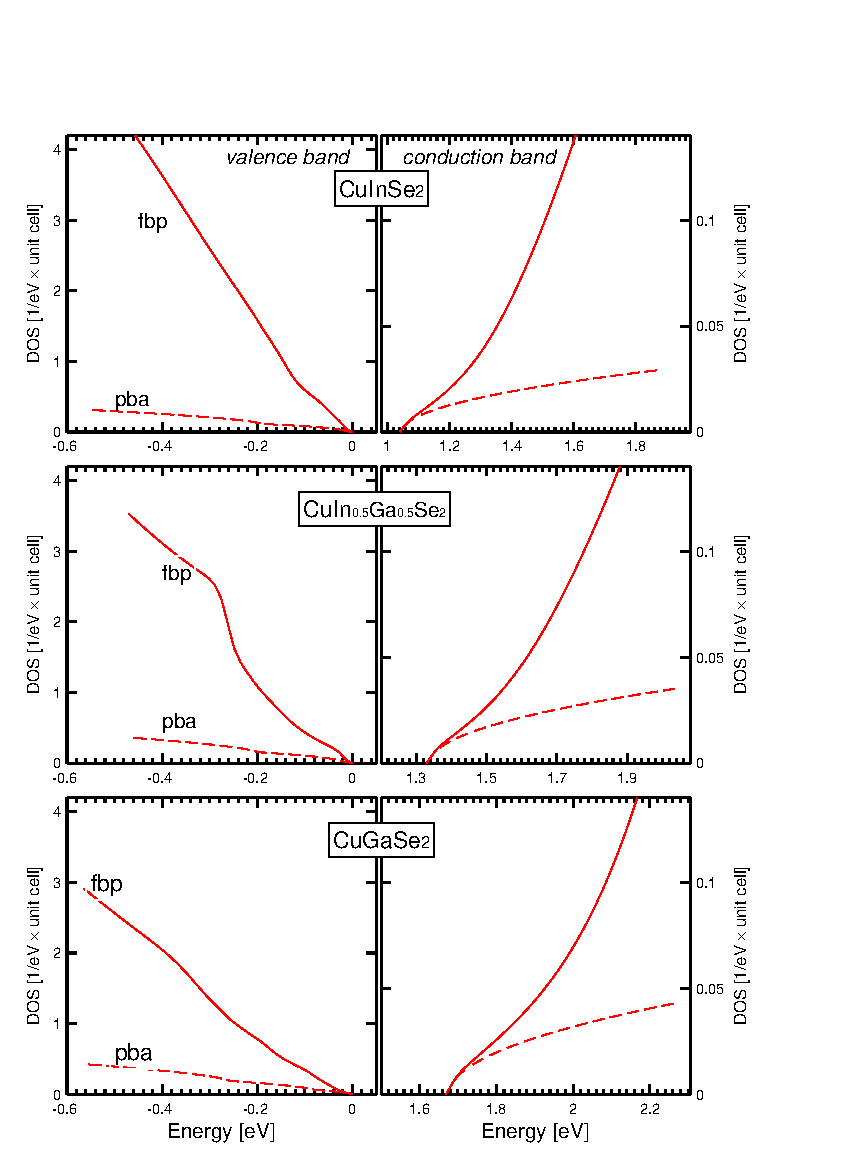
\includegraphics[width=0.48\textwidth,clip]{paper2figure4}
            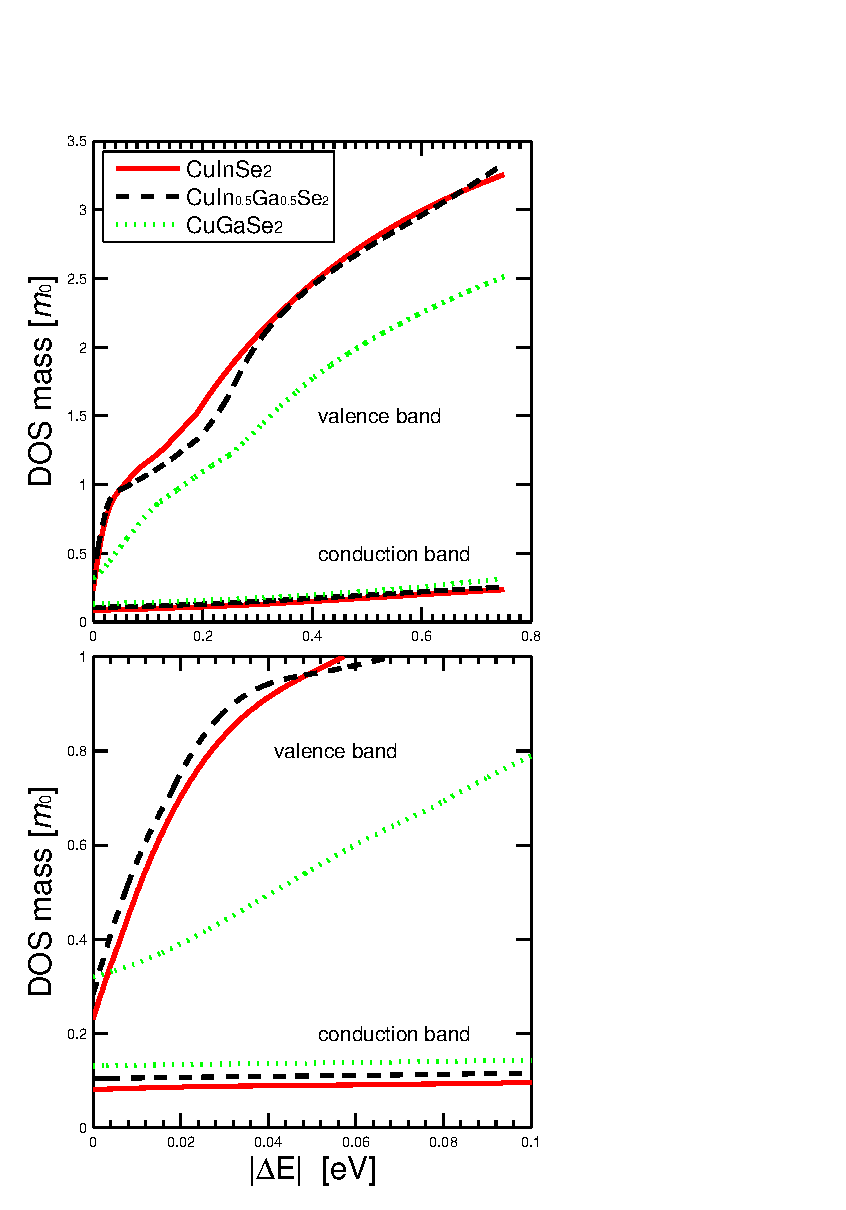
\includegraphics[width=0.46\textwidth,clip]{paper2figure6}
  %   \end{center}
    \caption{Left: Total DOS of the VBs and CB.The solid lines show the full band parameterization (fbp), and the dashed lines represent the parabolic band approximation (pba). Right:The DOS mass $m_{v/c}^{DOS}$ is calculated in the \textbf{Eq. \ref{dosmass}}. }
   \label{dost}
\end{figure}

The number of states with energies up to $E$ is obtained from the total DOS and the constant energy surfaces in \textbf{Fig. }. It shows that the VBs (CB) in Ga rich compounds will be less (more) populated by holes (electrons) for 
a given quasi-Fermi energy. It also demonstartes that the pba underestimates the band filling in the VBs and the CB strongly. For example, the number of VB states of CuInSe\textsubscript{2} is increased by a factor of around
18 at the positive energy $|\triangle E| = E_{v1}( \textbf{0})-E_{F,v}^* = 0.1 eV$ when the fba is included. For the CB, the number is incrased by a factor of around 3. At $|\triangle E| = 0.5 eV$, the incrase is as much as around 41
and 8 times, respectively.


 \begin{figure}[H]
 \centering
  %\begin{center}
            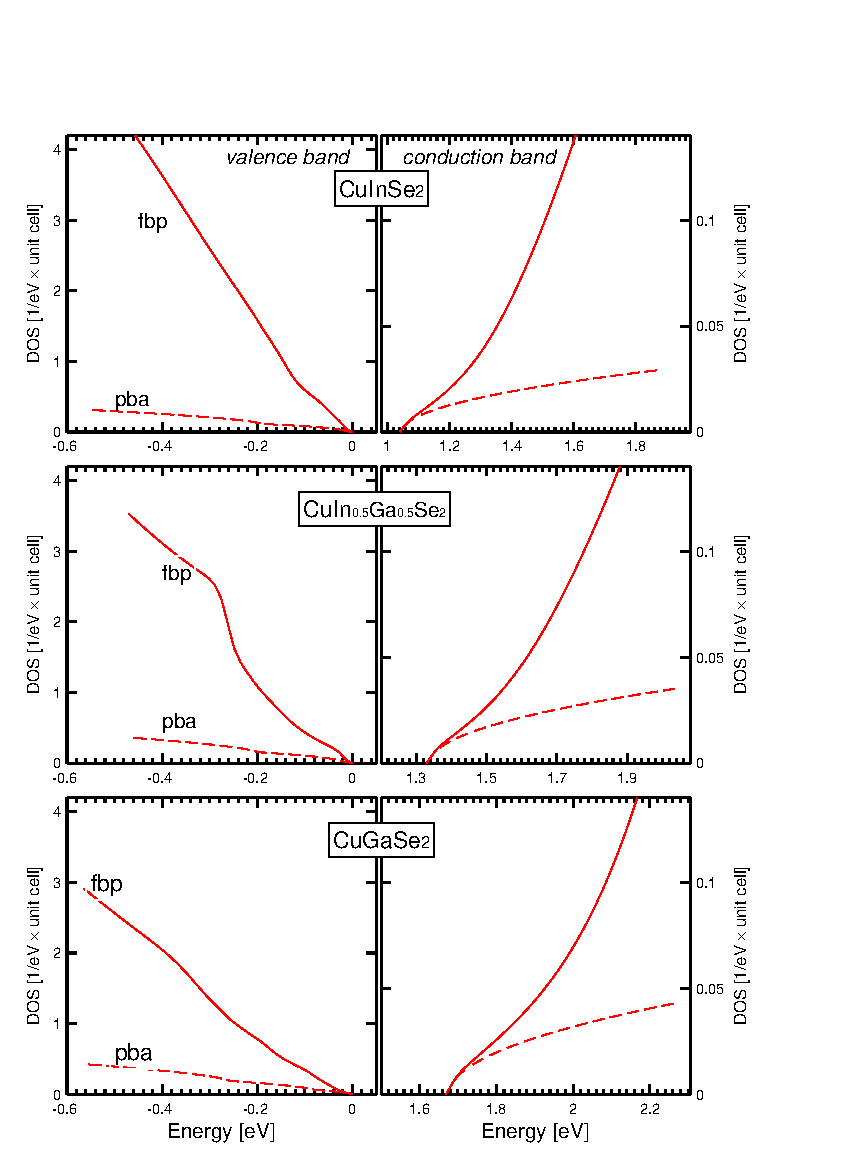
\includegraphics[width=0.48\textwidth,clip]{paper2figure4}
            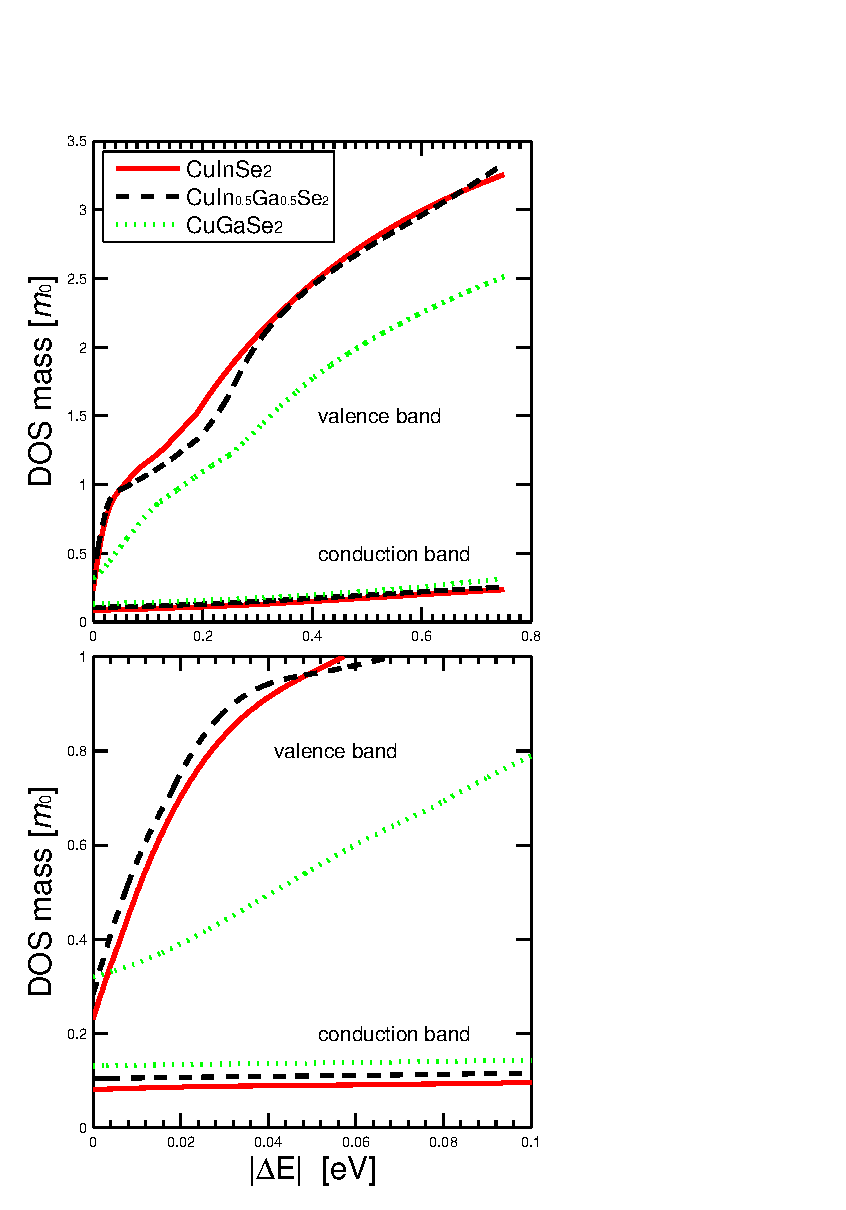
\includegraphics[width=0.46\textwidth,clip]{paper2figure6}
  %   \end{center}
 %   \caption{Carrier concentration \textit{p} or \textit{n} as functions of the quasi-Fermi energy $E_F^*$ of the VBs $E_{F,v}^*$ and of the CB $E_{F,c}^*$. Left column shows the results for large energy scale up to 0.5 eV, 
 %   and right column displays a close-up for small Fermi energies. In the figure, $|\delta E|$ is the positive energy difference $E_{v1}({0}) - E_{F,v}^*$ for the VBs and $E_{F,c}^* - E_{c1}({0})$ for the CB.The carrier
 %   concentrations consider external band filling in intrinsic materials at T = 0 K. The results demonstrate that the parabolic band approximation strongly underestimates the band filling of both the VBs and CB.}
 
 \caption{Carrier concentration \textit{p} or \textit{n} as functions of the quasi-Fermi energy  $E_F^*$ of the VBs  $E_{F,v}^*$ and of the CB $E_{F,c}^*$. Left column shows the results for large energy scale up to 0.5 eV,
 and right column displays a close-up for small Fermi energies. In the figure, $|\triangle E|$ is the positive energy difference $E_{v1}(\textbf{0})-E_{F,v}^*$ for the VBs and $E_{F,c}^*-E_{c1}(\textbf{0})$ for the CB.The carrier
 concentrations consider external band filling in intrinsic materials at T = 0 K. The results demonstrate that the parabolic band approximation strongly underestimates the band filling of both the VBs and CB.}
\end{figure}

The concentration of free holes $n_v(T)$ and free electrons $n_c(T)$ is calculated from the DOS by

\begin{equation}
\begin{split}
& n_v(T) = \int \limits_{-\infty}^{E_{v1}(\textbf{0})} g_v(E)(1-f(E))dE,\\
& n_c(T) = \int \limits_{E_{c1}(0)}^{\infty} g_c(E)f(E)dE.
\end{split}
\end{equation}

Here, $f(E) = 1/[1+exp{(E-E_F)/k_BT}]$ is the Fermi disctribution function. The intrinsic carrier concentration can be expressed as

\begin{equation}\label{cc}
 n_i(T) = \sqrt{n_c(T) \cdot n_v(T)}.
\end{equation}
 
The extrinsic carrier concentration for \textit{p}-type materials can be derived as:

\begin{equation}\label{ecc}
n_v(T) = \frac{n_i^2(T)}{n_v(T)} + \sum \limits_{\alpha} \frac{N_{A_{\alpha}}} {1+g_{A_{\alpha}} e^{ (\bigtriangleup_{A_{\alpha}}-E_F)/k_BT }}. 
\end{equation}

Here, $N_{A_{\alpha}}$ is the acceptor concentration of the $\alpha$th defect, $\bigtriangleup_{A_{\alpha}}$ implies the energy level of the acceptor state, and the $g_{A_{\alpha}}$
 is the spin degeneracy factor. The measured ionization energies for $V_{Cu}$ are utilized from Ref. ??.

The free carrier concentration in intrinsic for $\cigs$ (x = 0, 0.5, and 1) is obtained considering the temperature dependency of the band gaps (\textbf{Eq. \ref{bgtd}}).
The results from the pba for silicon (Si) and GaAs are compared with our simulation as well.

\begin{equation}\label{bgtd}
 E_g(T) = E_g(0) - \frac{a \cdot T^2}{b+T}.
\end{equation}

Here, parameters $a$ and $b$ are exploited from experimental values.

In \textbf{Fig. \ref{icc}}, the temperature dependent band gap and Fermi level (left panel) and intrinsic carrier concentration (right panel) are shown.  In the left panel of \textbf{Fig. \ref{icc}}, the band gap is 1.04, 1.33, and 1.67 eV for
CuIn\textsubscript{1-x}Ga\textsubscript{x}Se\textsubscript{2} where $x$ = 0, 0.5, and 1 at temperature around 0 K, respectively. Fermi level is exactly the mid-gap energy. The Fermi level changes only slightly with temperature. However, 
for CuInSe\textsubscript{2} and CuIn\textsubscript{0.5}Ga\textsubscript{0.5}Se\textsubscript{2}, the Fermi levels increase somewhat more compared with CuGaSe\textsubscript{2}. This is primarily due to the CB of DOS mass for 
CuGaSe\textsubscript{2} is almost the same, but the VB of DOS mass for CuGaSe\textsubscript{2} change smaller compared with CuInSe\textsubscript{2} and CuIn\textsubscript{0.5}Ga\textsubscript{0.5}Se\textsubscript{2} which will 
affect the DOS. As a consequence, the Fermi level is closer to the CB minimum in the In rich compounds. At T = 300 K and 600 K, the band-gap energies and Fermi energy are Eg (300) = 1.02, 1.29, and 1.62 eV, Eg (600) = 0.98, 1.24, 
and 1.55 eV, $E_F$ (300) = 0.55, 0.69, and 0.84 eV, and $E_F$ (600) = 0.59, 0.71, and 0.84 eV for x = 0, 0.5, and 1 respectively. In the right panel of \textbf{Fig. \ref{icc}}, the intrinsic carrier concentration is increased dramatically with the increasing of temperature for the $\cigs$. For example, in the case of $CuInSe_2$, the carrier concentration is
increased up to around $10^{5}$ times higher from temperture 300 K to 600 K. One also notice that the intrinsic carrier concentribution for the Si and $CuInSe_2$ are very comparable. The free carrier concentration is increased 
goes up to 2 $-$ 3 times by taking into account the non-parabolicity of the energy bands. 

 \begin{figure}[H]
    \begin{center}
            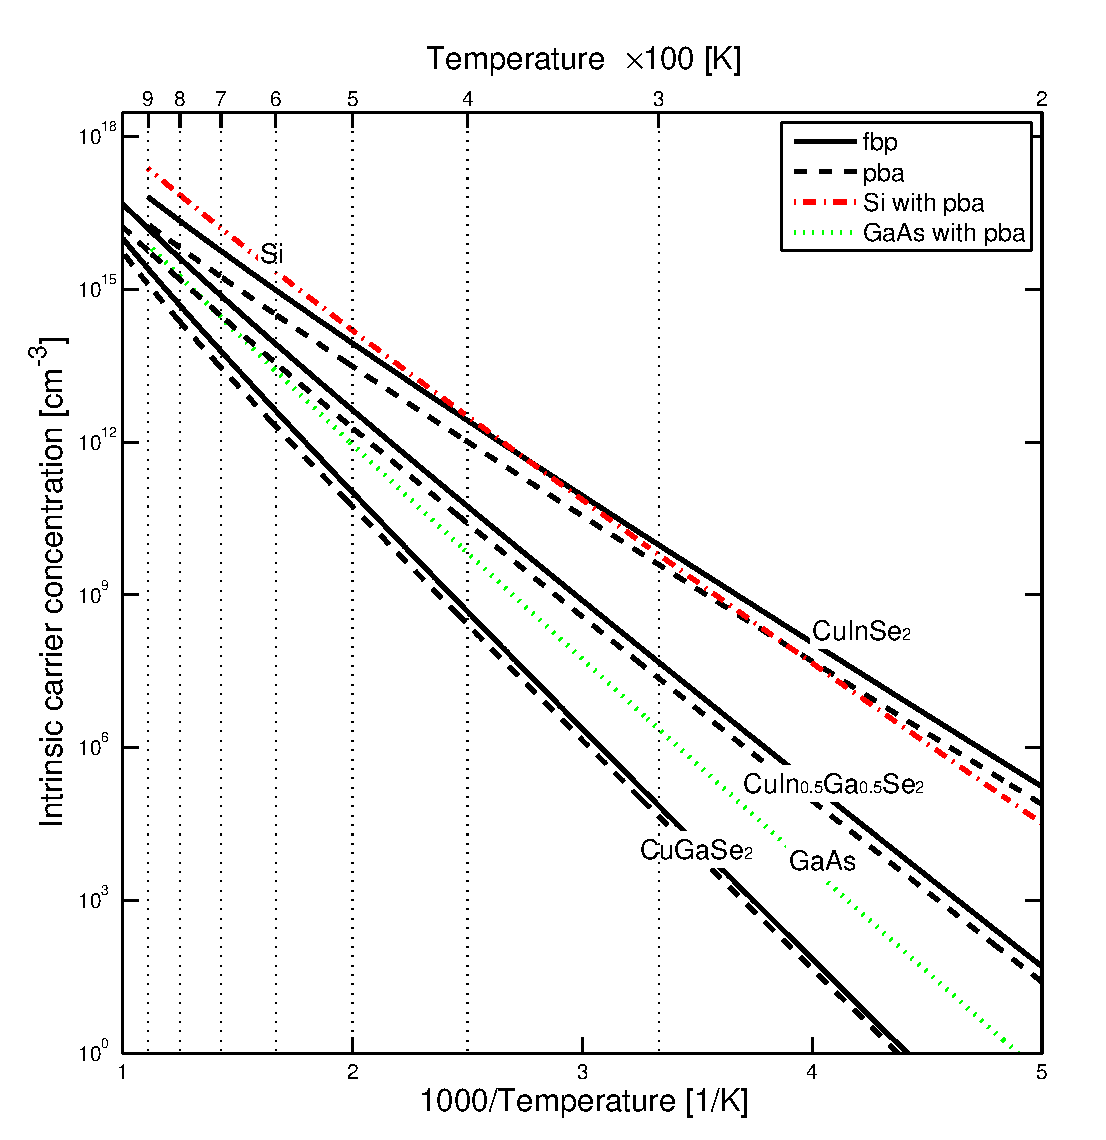
\includegraphics[width=0.5\textwidth,clip]{figure7b_1}
     \end{center}
    \caption{Intrinsic carrier concentration as function of temperature.}
   \label{icc}
\end{figure}




Since as-grown CuIn\textsubscript{1-x}Ga\textsubscript{x}Se\textsubscript{2} typically has \textit{p}-type character, the Fermi level and \textit{p}-type carrier concentration of free holes $n_v(T)$ and free electrons $n_c(T)$ is calculated by 
assuming the presences of the native Cu vacancies as acceptors. 


The calculated Fermi level $E_F^P$ in \textit{p}-type materials is presented in \textbf{Fig. \ref{ptypecc1}}, referred to the Fermi level of the intrinsic materials $E_F$ from \textbf{Fig. \ref{icc}}. Only at very high temperatures
( $T > 400 K$) and for low acceptor concentrations, the Fermi level of \textit{p}-type CuIn\textsubscript{1-x}Ga\textsubscript{x}Se\textsubscript{2} will reach the Fermi level of corresponding intrinsic compounds. Moreover, 
although the different compounds have comparable acceptor ionization energies, the Ga rich alloy has lower relative Fermi level; this is a direct consequence of the larger band gap of the Ga rich alloy. By comparing the calculations 
with the parabolic band approximation (dotted lines in \textbf{Fig. \ref{ptypecc1}} ) and the full band approach (solid lines) for each of the three CuIn\textsubscript{1-x}Ga\textsubscript{x}Se\textsubscript{2} alloys, one can notice
that the Femi level is similar for the two models only at low and at very high temperatures. In the mid-temperature region the difference is however apparent, especially for the high acceptor concentrations. Assuming parabolic bands
yields always a lower Fermi level. The reason for this effect is that the energy dependent effective mass $m_{v/c}^{DOS}(E)$ in the full band parameterization is always larger that the corresponding $\Gamma$-point mass. Although the
effect on the absolute value of the Fermi level seems to be small, it has an impact on the free carrier concentrations for highly doped materials. 

 \begin{figure}[H]
    \begin{center}
            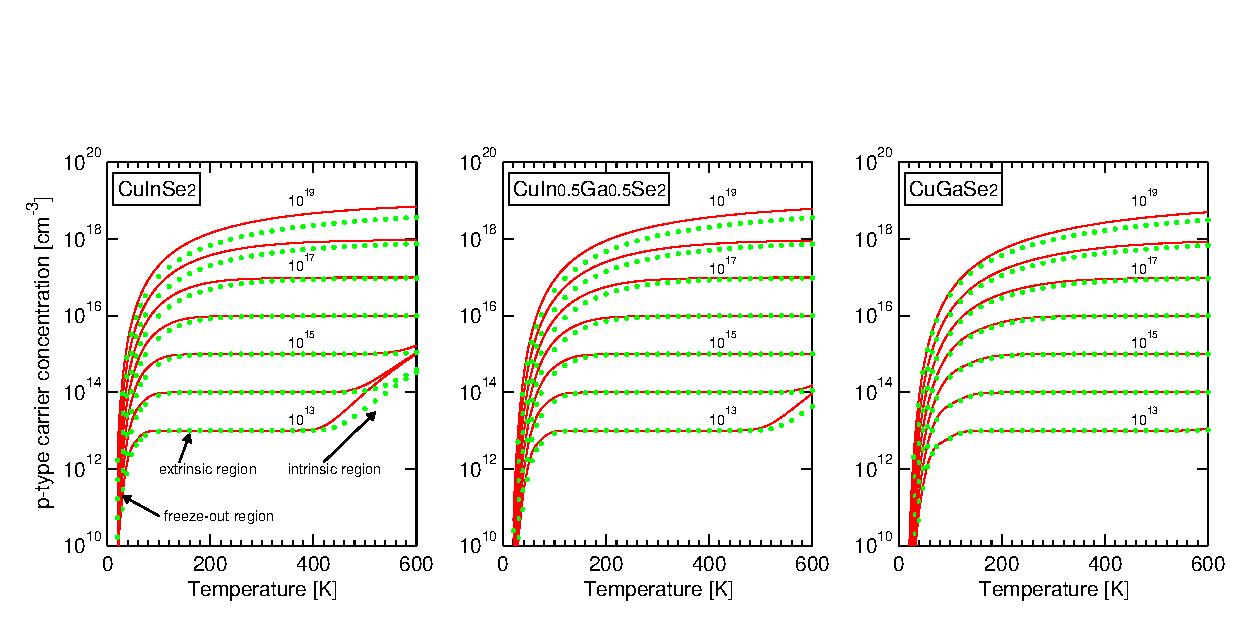
\includegraphics[width=1\textwidth,clip]{paper2figure9}
     \end{center}
    \caption{Fermi level as function of the temperature $20 \leq T \leq 600$ of \textit{p}-type CuInSe\textsubscript{2}, CuIn\textsubscript{0.5}Ga\textsubscript{0.5}Se\textsubscript{2}, and CuGaSe\textsubscript{2} for the effective
    doping concentration $N_A$ = $10^{13}$, $10^{14}$, $10^{15}$, $\cdot$, and $10^{19}$ acceptors/$cm^3$. The energy scale $E_F^p-E_F$ describes the Fermi energy with respect to the intrinsic $E_F$ (\textbf{Fig. \ref{icc}}).
    Dashed lines represent the VBM with respect to the intrinsic Fermi level. Solid and dotted lines represents the full band parameterization and the parabolic band approximation, respectively.}
   \label{ptypecc1}
\end{figure}




The p-type carrier concentration (\textbf{Fig. \ref{ptypecc}}) for $\cigs$ is presented using \textbf{Eq. \ref{ecc}}

 \begin{figure}[H]
    \begin{center}
            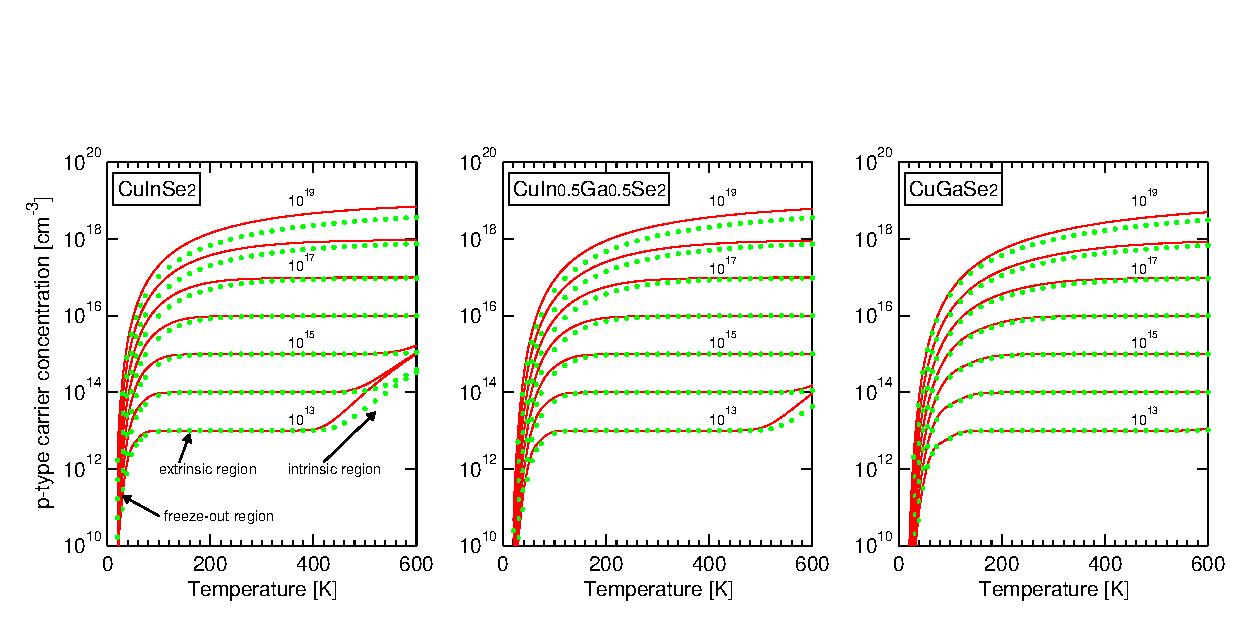
\includegraphics[width=1\textwidth,clip]{paper2figure9}
     \end{center}
    \caption{Free carrier concentration as function of the temperature in \textit{p}-type for $\mathrm{CuInSe_2}$, $\mathrm{CuIn_{0.5}Ga_{0.5}Se_2}$, and $\mathrm{CuGaSe_2}$.
    The effective doping concentration $N_A = 10^{13}, 10^{14}, 10^{15}$,..., and  $10^{19}$ acceptors/$cm^3$ are considered.}
   \label{ptypecc}
\end{figure}

From \textbf{Fig. \ref{ptypecc}}, the carrier concentration is recognized by three different regions: the freeze-out region, the extrinsic region and the intrinsic region. The 
transition from the freeze-out region to the extrinsic region happens below the room temperature except that the uncompensated acceptor concentration is above around 
$10^{18} cm^{-3}$. The transition from the extrinsic ergion to the intrinsic region for In rich compounds occurs at the lower temperature since they have smaller band gaps.
The result based on the pba underestimates the carrier concentration around by the factor of 2 in the both freeze-out and intrinsic regions. Therefore, the 
non-parabolic energy bands is required in order to describe the carrier concentration more accurately.


\section{Calculations of dielectric function for CIGS}
In this work, the dielectric function ($\varepsilon$) spectra of $CuIn_{0.5}Ga_{0.5}Se_2$ is calculated by the full-potential linearizaed augmented plane wave (FPLAPW) method using the generalized gradient approximation (GGA)
plus an onsite Coulomb interaction $U$ of the Cu $d$ states. Afterwards, the different contributions to $\varepsilon_2$ (Im$(\varepsilon)$) in terms of the transitions between the valence bands and the conduction bands are identified. At last, 
the $\textbf{k}$-dependence of the interband critical points (CPs) along the main symmetry directions is analyzed. The result is compared with experimental work ($CuIn_{0.7}Ga_{0.3}Se_2$) at temperature of 40 K and 300 K,
and they are in a good agreement.

 \begin{figure}[H]
    \begin{center}
            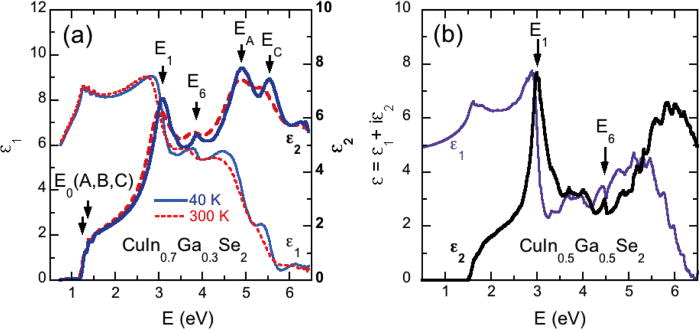
\includegraphics[width=1\textwidth]{111111.png}
     \end{center}
    \caption{Left panel: The real ($\varepsilon_1$) and imaginary ($\varepsilon_2$) part of dielectric function spectra for $CuIn_{0.7}Ga_{0.3}Se_2$ 
at 40 K (solid blue line) and 300 K (dashed red lines). Four prominent CP features are shown. Right panel: the dielectric function spectra for  $CuIn_{0.5}Ga_{0.5}Se_2$
calculated by FPLAPW method at 0 K. The major CP features are identified. }
   \label{df1}
\end{figure}

From \textbf{Fig. \ref{df1}}, one will notice that the general shape between experimental and calculated result is similar. The calculation indicates that there is no big 
difference in the optical properties for those two materials, except the shift of CP energies.
 
The analysis based on experimental work indicates that there are twelve CPs from 2.5 eV to 6.4 eV. The electronic origin for each CP is analyzed based on the calculated 
result. First, the contribution to dielectric function between the valence bands and conduction bands is presented.

 \begin{figure}[H]
    \begin{center}
            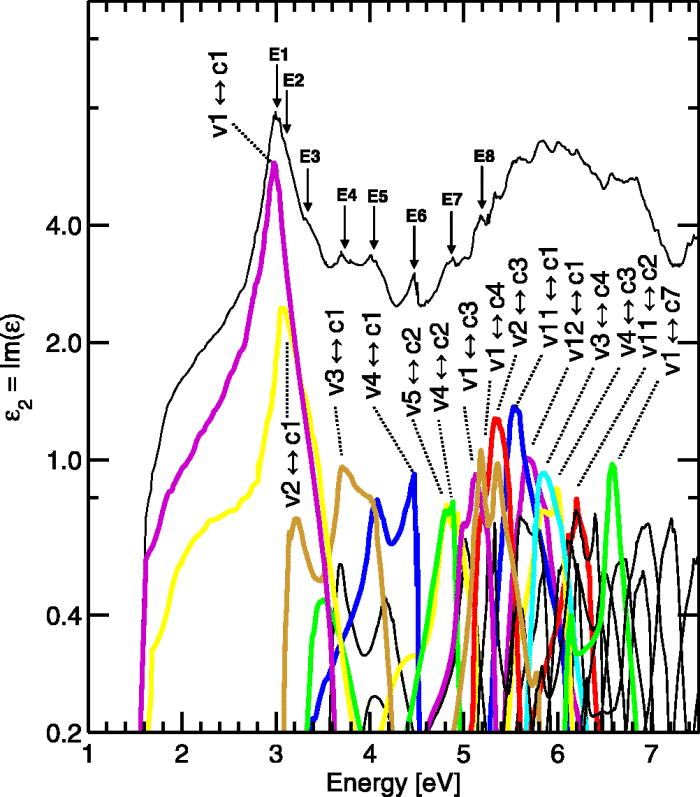
\includegraphics[width=0.5\textwidth]{222222}
     \end{center}
    \caption{Band-to-band analysis of the contribution to the total $\varepsilon_2$ spectrum. The vertical axis is in the log scale.}
   \label{df2}
\end{figure}

Here, $v_1$ and $c_1$ represent the topest valence band and lowest conduction band, respectively. From the \textbf{Fig. \ref{df2}} and \textbf{Fig. \ref{df3}}, one will notice that the $E_1$ CP comes from 
the $v_1 \longrightarrow c_1$
transition near the P(1/2, 1/2, 1/2) point of the brillouin zone (BZ). The $E_2$ and $E_3$ CPs are corresponding to transition of $v_2 \longrightarrow c_1$ in the P point
as well in the BZ.
 The $E_2$ and $E_3$ CPs are small peak in the \textbf{Fig. \ref{df2}}. However, the calculation of $CuInSe_2$ indicates that they happens 0.1$-$0.2 eV higher than 
the $E_1$ CP, which is distinct spectral features (\textbf{Fig. \ref{ccccc}}). The $E_4$ CP comes from the transition of $v_3 \longrightarrow c_1$ at the $M (1,0,0) = M^*(0,0,1)$ point.
The $E_5$ CP is contributed by the transitions $v_4 \longrightarrow c_1$ at the $N (1/2,0,1/2)$ point and $v_3 \longrightarrow c_1$ at the $M/M^*$ point. The $E_6$ CP feature
corresponding to the  $v_4 \longrightarrow c_1$ at the $N$ point. The $E_7$ is from the transitions $v_4 \longrightarrow c_2$ at the $\Gamma (0,0,0)$ and N point, the 
  $v_5 \longrightarrow c_2$ at the $\Gamma$ point is also contributed.
 \begin{figure}[H]
    \begin{center}
            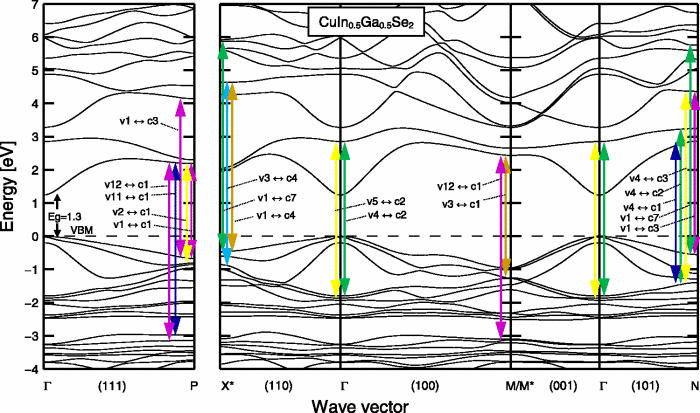
\includegraphics[width=0.8\textwidth]{333333}
     \end{center}
    \caption{Band-to-band analysis of the contribution to the total $\varepsilon_2$ spectrum. The vertical axis is in the log scale.}
   \label{df3}
\end{figure}

\begin{figure}[H]
\begin{center}
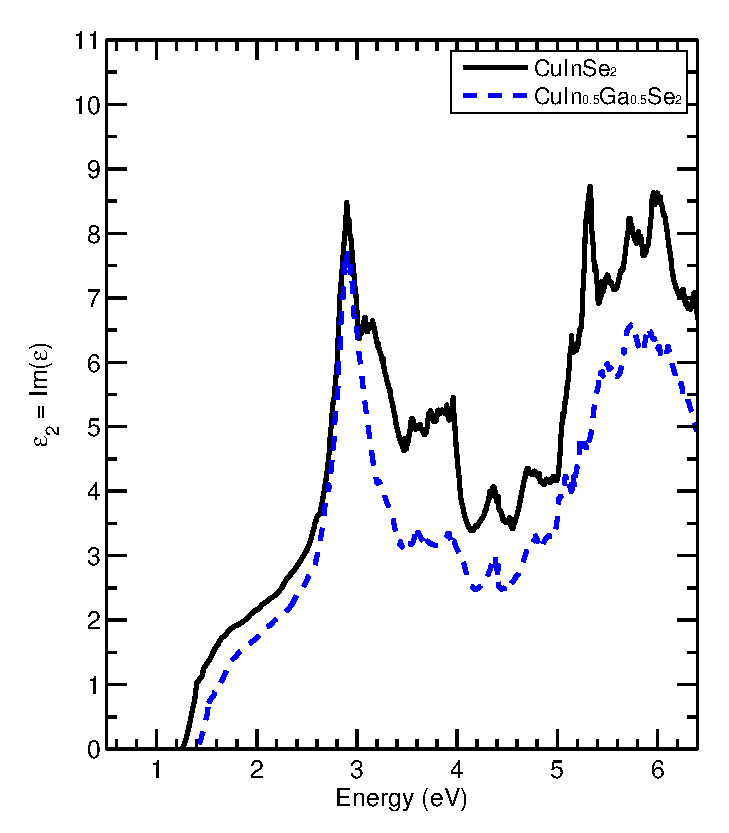
\includegraphics[scale=0.7]{thesis2.eps}
\end{center}
\caption{The $\varepsilon_2$ spectra for ${\mathrm{ CuInSe_2}}$ and $\mathrm {CuIn_{0.5}Ga_{0.5}Se_2}$. }
\label{ccccc}
\end{figure}


\chapter{Summary of the publications}

\begin{comment}
\section{Methodology and implementation}

\subsection{scalar relativistic approximation}

\subsubsection{Implementation}
In this section, the Hamiltonian matrix using scalar relativistic approximation (SRA) term in the Pauli Hamiltonian is derived in the muffin tin (MT) 
region and interstitial region (IR). From the section \ref{srasoc}, the SRA Hamiltonian term is defined:

\begin{equation}
  H_{sra} = - \frac{\bigtriangledown^4}{8c^2} + \frac{\bigtriangledown^2 V(r)}{8c^2}.
\end{equation}

The Hamiltonian matrix can be implemented by:

\begin{equation}
\label{sra1}
 H_{jj'} = \left  < \phi_{j} | H_{sra} | \phi_{{j'}} \right >,
\end{equation}
 
where $\phi_j$ is the basis function. The basis function will be divided into two types in the Exciting code (FPLAPW method), one is in the muffin tin (MT) region, the other is in the interstitial region. Especially,
the basis function has two forms in the MT region, one is augemented plane wave, another is local orbitals. 

In the MT region, the basis function is:
\begin{equation}
\begin{split}
& \phi_{{\textbf{G}}}^{APW} = \sumg<\alpha>\sum\limits_{{\ell}m} A _{{\ell}m}^{\alpha} {(\textbf{k+G})} u_{{\ell}}(r_{\alpha}, E_{\ell}) Y_{{\ell}m}(\hat{\textbf{r}}_{\alpha}), \\
& \phi_{{{p}}}^{lo} = v_p^{\alpha}(r) Y_{{\ell}_p m_p}(\hat{\textbf{r}}_{\alpha} ) = \sum\limits_{j=1}^{M_p^{\alpha}} B _j^{\alpha} w_j(r_\alpha) Y_{{\ell}_p m_p}(\hat{\textbf{r}}_{\alpha} ),
\end{split}
\end{equation}

where $\phi_{{\textbf{G}}}^{APW}$ and $\phi_{{{p}}}^{lo}$ are the basis function in the MT region. The $A _{{\ell}m}^{\alpha} {(\textbf{k+G})}$ and $B _j^{\alpha}$ are
the match coefficient. The $u_{{\ell}}^{\alpha}(r_{\alpha}, E_{\ell})$ and $w_j(r_\alpha)$ are the radial function, the $Y_{{\ell}m}(\hat{\textbf{r}}_{\alpha})$ and $Y_{{\ell}_p m_p}(\hat{\textbf{r}}_{\alpha})$
are spherical harmonics.

In the interstitial region, the basis function is:
\begin{equation}
 \phi_{{\textbf{G}}}^{IR} =  \frac {1}{\sqrt{\Omega}} e^{i({ \textbf {k+G}}) {\textbf r}}. 
\end{equation}

Therefore the standard Hamiltonian matrix (without considering local orbital) in the MT region  is:
\begin{equation}
\label{sra111}
\begin{split}
& H_{jj'}^{MT\_{AA}} =  \left  < \phi_{\textbf{G}}^{APW} | H_{sra} | \phi_{\textbf{G'}}^{APW} \right > 
\end{split}
\end{equation}

In Eq. \ref{sra111}, the main part is to calculate:

\begin{equation}
\label{sra222}
\begin{split}
& \left  < u_{{\ell}}(r_{\alpha}, E_{\ell}) Y_{{\ell}m}(\hat{\textbf{r}}_{\alpha}) | - \frac{\bigtriangledown^4}{8c^2} + \frac{\bigtriangledown^2 V(r)}{8c^2} | u_{{\ell'}}(r_{\alpha}, E_{\ell'}) Y_{{\ell'}m'}(\hat{\textbf{r}}_{\alpha}) \right > \\
& = \left  < u_{{\ell}}(r_{\alpha}, E_{\ell}) Y_{{\ell}m}(\hat{\textbf{r}}_{\alpha}) | - \frac{\bigtriangledown^4}{8c^2} | u_{{\ell'}}(r_{\alpha}, E_{\ell'}) Y_{{\ell'}m'}(\hat{\textbf{r}}_{\alpha}) \right > \\ 
&    + \left  < u_{{\ell}}(r_{\alpha}, E_{\ell}) Y_{{\ell}m}(\hat{\textbf{r}}_{\alpha}) |  \frac{\bigtriangledown^2 V(r)}{8c^2} | u_{{\ell'}}(r_{\alpha}, E_{\ell'}) Y_{{\ell'}m'}(\hat{\textbf{r}}_{\alpha}) \right > \\
& =- \frac{1}{8c^2} \left  < \bigtriangledown^2 \big (u_{{\ell}}(r_{\alpha}, E_{\ell}) Y_{{\ell}m}(\hat{\textbf{r}}_{\alpha}) \big ) | \bigtriangledown^2 \big ( u_{{\ell'}}(r_{\alpha}, E_{\ell'}) Y_{{\ell'}m'}(\hat{\textbf{r}}_{\alpha}) \big )\right > \\
&    + \frac{1}{8c^2} C_{\ell m,\ell'm'}^{\ell_\wedge m_\wedge}\int \limits_{0}^{R_{\alpha}} u_{{\ell}}(r_{\alpha}, E_{\ell}) \overline{V}_{l_\wedge m_\wedge} u_{{\ell'}}(r_{\alpha}, E_{\ell'}) d r \\
& = -\frac{1}{8c^2} \delta_{\ell \ell'}\delta_{m m'} \int \limits_{0}^{R_{\alpha}} \bigtriangledown^2_r u_{{\ell}}(r_{\alpha}, E_{\ell})   \bigtriangledown^2_r u_{{\ell'}}(r_{\alpha}, E_{\ell'}) r_{\alpha}^2 dr \\
& +  \frac{1}{4c^2} \delta_{\ell \ell'}\delta_{m m'} \ell'(\ell'+1) \int \limits_0^{R_{\alpha}} \bigtriangledown_r u_{{\ell}}(r_{\alpha}, E_{\ell}) \bigtriangledown_r u_{{\ell'}}(r_{\alpha}, E_{\ell'}) d r \\
& -  \frac{1}{8c^2} \delta_{\ell \ell'}\delta_{m m'} \ell(\ell+1) \ell(\ell+1) \int \limits_0^{R_{\alpha}}  u_{{\ell}}(r_{\alpha}, E_{\ell})  u_{{\ell'}}(r_{\alpha}, E_{\ell'}) \frac{1}{r_{\alpha}^2} d r \\
& +  \frac{1}{8c^2} C_{\ell m,\ell' m'}^{\ell_\wedge m_\wedge}\int \limits_{0}^{R_{\alpha}} u_{{\ell}}(r_{\alpha}, E_{\ell}) \overline{V}_{l_\wedge m_\wedge} u_{{\ell'}}(r_{\alpha}, E_{\ell'}) r_{\alpha}^2  d r 
\end{split}
\end{equation}

where

\begin{equation}
\begin{split}
& \bigtriangledown^2 \{ V(r) \} \\
& = \bigtriangledown^2 \{ \sum \limits_{\ell_\wedge m_\wedge} V_{\ell_\wedge m_\wedge} Y_{{\ell_\wedge } m_\wedge}(\hat{\textbf{r}}_{\alpha})\} \\
& = \sum \limits_{\ell_\wedge m_\wedge} \overline{V}_{\ell_\wedge m_\wedge} Y_{{\ell_\wedge } m_\wedge}(\hat{\textbf{r}}_{\alpha}),
\end{split}
\end{equation}

and $C_{\ell m,\ell' m'}^{\ell_\wedge m_\wedge}$ in equation \ref{sra222} is the Gaunt coefficients.

It is similar to consider the local orbitals:

\begin{equation}
\begin{split}
& H_{jj'}^{MT\_{ALo}} =  \left  < \phi_{\textbf{G}}^{APW} | H_{sra} | \phi_{p}^{lo} \right > 
\end{split}
\end{equation}

The main part to be calculated is:

\begin{equation}
\label{sra333}
\begin{split}
& \frac{1}{8c^2} \left  < \bigtriangledown^2 \big (u_{{\ell}}(r_{\alpha}, E_{\ell}) Y_{{\ell}m}(\hat{\textbf{r}}_{\alpha}) \big ) | \bigtriangledown^2 \big (w_j(r_\alpha)) Y_{{\ell_p}m_p}(\hat{\textbf{r}}_{\alpha}) \big )\right > \\
&    + \frac{1}{8c^2} C_{\ell m,\ell_p m_p}^{\ell_\wedge m_\wedge}\int \limits_{0}^{R_{\alpha}} u_{{\ell}}(r_{\alpha}, E_{\ell}) \overline{V}_{l_\wedge m_\wedge} w_j(r_\alpha) d r \\
& = -\frac{1}{8c^2} \delta_{\ell \ell_p}\delta_{m m_p} \int \limits_{0}^{R_{\alpha}} \bigtriangledown^2_r u_{{\ell}}(r_{\alpha}, E_{\ell})   \bigtriangledown^2_r w_j(r_\alpha) r_{\alpha}^2 dr \\
& +  \frac{1}{4c^2} \delta_{\ell \ell_p}\delta_{m m_p} \ell_p(\ell_p+1) \int \limits_0^{R_{\alpha}} \bigtriangledown_r u_{{\ell}}(r_{\alpha}, E_{\ell}) \bigtriangledown_r w_j(r_\alpha)   d r \\
& -  \frac{1}{8c^2} \delta_{\ell \ell_p}\delta_{m m_p} \ell(\ell+1) \ell_p(\ell_p+1) \int \limits_0^{R_{\alpha}}  u_{{\ell}}(r_{\alpha}, E_{\ell}) w_j(r_\alpha) \frac{1}{r_{\alpha}^2} d r \\
& +  \frac{1}{8c^2} C_{\ell m,\ell_p m_p}^{\ell_\wedge m_\wedge}\int \limits_{0}^{R_{\alpha}} u_{{\ell}}(r_{\alpha}, E_{\ell}) \overline{V}_{l_\wedge m_\wedge} w_j(r_\alpha) r_{\alpha}^2  d r. 
\end{split}
\end{equation}

And

\begin{equation}
\begin{split}
& H_{jj'}^{MT\_{LoA}} =  \left  < \phi_{p}^{lo}   | H_{sra} | \phi_{\textbf{G}}^{APW} \right > 
\end{split}
\end{equation}
The main part to be calculated is:

\begin{equation}
\label{sra222}
\begin{split}
&  \left  < w_j(r_\alpha) Y_{{\ell_p}m_p}(\hat{\textbf{r}}_{\alpha}) | - \frac{\bigtriangledown^4}{8c^2} | u_{{\ell'}}(r_{\alpha}, E_{\ell'}) Y_{{\ell'}m'}(\hat{\textbf{r}}_{\alpha}) \right > \\ 
&    + \left  <  w_j(r_\alpha) Y_{{\ell_p}m_p}(\hat{\textbf{r}}_{\alpha}) |  \frac{\bigtriangledown^2 V(r)}{8c^2} | u_{{\ell'}}(r_{\alpha}, E_{\ell'}) Y_{{\ell'}m'}(\hat{\textbf{r}}_{\alpha}) \right > \\
& = \frac{1}{8c^2} \left  < \bigtriangledown^2 \big ( w_j(r_\alpha) Y_{{\ell_p}m_p}(\hat{\textbf{r}}_{\alpha}) \big ) | \bigtriangledown^2 \big ( u_{{\ell'}}(r_{\alpha}, E_{\ell'}) Y_{{\ell'}m'}(\hat{\textbf{r}}_{\alpha}) \big )\right > \\
&    + \frac{1}{8c^2} C_{\ell_p m_p,\ell'm'}^{\ell_\wedge m_\wedge}\int \limits_{0}^{R_{\alpha}} w_j(r_\alpha) \overline{V}_{l_\wedge m_\wedge} u_{{\ell'}}(r_{\alpha}, E_{\ell'}) d r \\
& = - \frac{1}{8c^2} \delta_{\ell_p \ell'}\delta_{m_p m'} \int \limits_{0}^{R_{\alpha}} \bigtriangledown^2_r w_j(r_\alpha)   \bigtriangledown^2_r u_{{\ell'}}(r_{\alpha}, E_{\ell'}) r_{\alpha}^2 dr \\
& +  \frac{1}{4c^2} \delta_{\ell_p \ell'}\delta_{m_p m'} \ell'(\ell'+1) \int \limits_0^{R_{\alpha}} \bigtriangledown_r w_j(r_\alpha) \bigtriangledown_r u_{{\ell'}}(r_{\alpha}, E_{\ell'}) d r \\
& -  \frac{1}{8c^2} \delta_{\ell_p \ell'}\delta_{m_p m'} \ell_p(\ell_p+1) \ell'(\ell'+1) \int \limits_0^{R_{\alpha}}  w_j(r_\alpha)  u_{{\ell'}}(r_{\alpha}, E_{\ell'}) \frac{1}{r_{\alpha}^2} d r \\
& +  \frac{1}{8c^2} C_{\ell_p m_p,\ell' m'}^{\ell_\wedge m_\wedge}\int \limits_{0}^{R_{\alpha}} w_j(r_\alpha) \overline{V}_{l_\wedge m_\wedge} u_{{\ell'}}(r_{\alpha}, E_{\ell'}) r_{\alpha}^2  d r 
\end{split}
\end{equation}

And 

\begin{equation}
\begin{split}
& H_{jj'}^{MT\_{LoLo}} =  \left  <\phi_{p}^{lo}  | H_{sra} | \phi_{p'}^{lo} \right > 
\end{split}
\end{equation}
The main part to be calculated is:

\begin{equation}
\label{sra444}
\begin{split}
& \frac{1}{8c^2} \left  < \bigtriangledown^2 \big (w_j(r_\alpha) Y_{{\ell_p}m_p}(\hat{\textbf{r}}_{\alpha}) \big ) | \bigtriangledown^2 \big (w_{j'}(r_\alpha)) Y_{{\ell_{p'}}m_{p'}}(\hat{\textbf{r}}_{\alpha}) \big )\right > \\
&    + \frac{1}{8c^2} C_{\ell_p m_p,\ell_{p'} m_{p'}}^{\ell_\wedge m_\wedge}\int \limits_{0}^{R_{\alpha}} w_j(r_\alpha) \overline{V}_{l_\wedge m_\wedge} w_{j'}(r_\alpha) d r \\
& = - \frac{1}{8c^2} \delta_{\ell_p \ell_{p'}}\delta_{m_p m_{p'}} \int \limits_{0}^{R_{\alpha}} \bigtriangledown^2_r w_j(r_\alpha)   \bigtriangledown^2_r w_{j'}(r_\alpha) r_{\alpha}^2 dr \\
& +  \frac{1}{8c^2} \delta_{\ell_p \ell_{p'}}\delta_{m_p m_{p'}} \ell_{p'}(\ell_{p'}+1) \int \limits_0^{R_{\alpha}} \bigtriangledown_r w_j(r_\alpha) \bigtriangledown_r w_{j'}(r_\alpha) d r \\
& -  \frac{1}{8c^2} \delta_{\ell_p \ell_{p'}}\delta_{m_p m_{p'}} \ell_{p}(\ell_{p}+1) \ell_{p'}(\ell_{p'}+1) \int \limits_0^{R_{\alpha}}  w_j(r_\alpha) w_{j'}(r_\alpha) \frac{1}{r_{\alpha}^2} d r \\
& +  \frac{1}{8c^2} C_{\ell_p m_p,\ell_{p'} m_{p'}}^{\ell_\wedge m_\wedge}\int \limits_{0}^{R_{\alpha}} w_j(r_\alpha) \overline{V}_{l_\wedge m_\wedge} w_{j'}(r_\alpha) r_{\alpha}^2 d r 
\end{split}
\end{equation}

In the interstial region:

\begin{equation}
\begin{split}
& H_{jj'}^{IR} =  \left  < \phi_{\textbf{j}}^{IR} | H_{sra} | \phi_{\textbf{j'}}^{IR} \right > \\
&              = \left  < \phi_{{\textbf{G}}}^{IR}  | H_{sra} | \phi_{{\textbf{G'}}}^{IR} \right > \\
&              =  \frac{1}{{8 {c}^2 }} \{ -(k+G)^2(k+G')^2 \widetilde{\theta}_{I}(G-G') -  \sumg<G''> V_{G''}(G'')^2 \widetilde{\theta}_{I}(G-G'-G'') \}
\end{split}
\end{equation}

where potential is defined in the section \ref{epote}. And if $\theta_{I}(r)$ is the characteristic function of the interstitial region ( $r$ included in MT, $\theta_{I}(r)$ = 0, otherwise it is 1), $\widetilde{\theta}_{I}(r)$ comes from the Fourier transform of $\theta_{I}(r)$:
\begin{equation}
\theta_{I}(r) = \sumg<G> \widetilde{\theta}_{I}(G) \expg<G>
\end{equation}

And $\widetilde{\theta}_{I}(G)$ is defined:
 
\begin{equation*}\label{ap1}
\widetilde{\theta}_{I}(G) =
\begin{cases}  \delta_{G,0}-\sumg<\alpha> \frac{4 \pi R_{\alpha}^{3}}{\Omega} \frac{j_1(|G|R_{\alpha})}{|G|R_{\alpha}} e^{-iGr_{\alpha}} & \quad \mbox{if $\textbf{G} \leqslant \textbf{G}_{max} $}
\\
0  & \quad \mbox{if $\textbf{G} > \textbf{G}_{max} $}\\ 
\end{cases}
\end{equation*}

where $R_{\alpha}$ is the radius of the MT, $r_{\alpha}$ is the position refer to the $\alpha$th atom, and $j_1$ is the ${1}$st order Bessel function.

\subsubsection{Results and discusstion}
It is needed to insert more after getting some results.

\subsection{Scalar relativistic approximation in k $\cdot$ p method}
\subsubsection{Implementation}
One can check the section \ref{kpmaa} for the introduction of \textbf{k $\cdot$ p} method. Here the relativistic KS equation for \textbf{k $\cdot$ p} method in atomic units can be expressed as:

\begin{equation}\label{m1}
\left\{ - \frac{\bigtriangledown^2}{2} + V(r) - \frac{\bigtriangledown^4}{8c^2} + \frac{\bigtriangledown^2 V(r)}{8c^2} \right\} \wfbloch<n>< \bold k> = \ebloch<n><\bold k> \wfbloch<n><\bold k>,
\end{equation}

where 

\begin{equation}\label{m2}
\begin{split}
& \wfbloch<n><\bold k> =  {\sum\limits_{j}} C_{n,j}^{\bold k} \chikp<j><\bold k>, \\
& \chikp<j><\textbf k> = \expg<(\bold k-\bold {k_0})>  \wfbloch<j><\bold {k_0}>.
\end{split}
\end{equation}

One can follow almost the same derivation but with more terms in the section \ref{kpmaa}, which ends up:

\begin{equation}\label{m4}
{\sum\limits_{j}} C_{n,j}^{\bold {k}} \left \{ H_{j',j}- \ebloch<n><\bold {k}> \delta_{j',j} \right \} =0,
\end{equation}

where
\begin{equation} \label{m5}
\begin{split}
& H_{j',j} = \left \{  \ebloch<j><\bold {k_0}>  + \frac{1}{2} { (\bold{k}-\bold{k}_0)^2} - \frac{1}{8c^2}(\bold{k}-\bold{k}_0)^4   \right \} \delta_{j',j} + \left \{ {-i(\bold{k}-\bold{k}_0) + \frac{i}{2c^2}(\bold{k}-\bold{k}_0)^3} \right \} {\textbf p_{j',j}} \\
& \qquad  + \left \{ \frac{3}{4c^2}(\bold{k}-\bold{k}_0)^2  \right \} {\textbf p'_{j',j}} + \left \{ \frac{-i}{2c^2}(\bold{k}-\bold{k}_0) \right \} {\textbf p''_{j',j}}, 
\end{split}
\end{equation}

and

\begin{equation} 
\begin{split}
& {\textbf p_{j',j}} = \langle \wfbloch<j'>< \bold k_0>| {\bigtriangledown} | \wfbloch<j>< \bold k_0>  \rangle, \\
& {\textbf p'_{j',j}} = \langle \wfbloch<j'>< \bold k_0>| {\bigtriangledown^2} | \wfbloch<j>< \bold k_0>  \rangle, \\
& {\textbf p''_{j',j}} = \langle \wfbloch<j'>< \bold k_0>| {\bigtriangledown^3} |\wfbloch<j>< \bold k_0>  \rangle.
\end{split}
\end{equation}

From the above Eq. \ref{m4}, the coefficient $ C_{n,j}^{\bold k}$ and $\ebloch<n><\bold {k}>$ are calculated.

\subsubsection{Results and discussion}

It is needed to insert more after getting some results.

\subsection{Spin-orbit coupling}

\subsubsection{Implementation}
In this section, spin-orbit coupling (SOC) implementation is derived in the muffin tin (MT) region and interstial region (IR). In the MT region, this implementation is compared with 
the method exsiting in the orignal Exciting code.

First, the way to implemente the SOC in the Exciting code is presented, which is included in second-variational scheme, that means it takes use of the basis function which is expanded from the first variational wavefunction.
\begin{equation}
\begin{split}
 & \widehat{H}_{1}   \phi^{i}_{1}  = E^{i}_1  \phi^{i}_{1} \\
 & (\widehat{H}_1+\widehat{H}_{soc})  \Psi  = E \Psi
\end{split}
\end{equation}
\noindent  where $ \widehat{H}_{1}$ and $ \phi^{i}_{1}$ are first variational \hm and wavefunction, respectively, and $\Psi = \sumi<i> c_{i} \phi^{i}_1$.
If  multiply $\phi^{j}_{1}$ on the left side of the second item of the above equation.
\begin{equation}
\begin{split}
 & <  \phi^{j}_1 |(\widehat{H}_1+\widehat{H}_{soc}) | \sumi<i> c_{i} \phi^{i}_1 > = E< \phi^{j}_1 | \sumi<i> c_{i} \phi^{i}_1>
\end{split}
\end{equation}

\noindent After some operations, the above equation becomes:
\begin{equation}
\begin{split}
 &\sumi<i> c_{i} \{ E^{i}_{1} \delta_{i,j} +<\phi^{j}_1 |\widehat{H}_{soc} | \phi^{i}_1  > \} = \sumi<i> c_{i} E \delta_{i,j}
\end{split}
\end{equation}
 
\noindent So finally, the above equation becomes the eigenvalue probelm $H_2 C = E C$.
\begin{equation}\label{ep444}
H_2=\left[
\begin{matrix}
    E_1+H_{11} & H_{12} & \cdots & H_{1N} \\
    H_{21} & E_2 + H_{22} & \cdots & H_{2N} \\
    \vdots               & \vdots               &        & \vdots               \\
     H_{N1} & H_{N2} & \cdots & E_{N}+H_{NN} \\
\end{matrix} \right],
C = \left[ \begin{array}{c} c_1 \\ c_2 \\ \vdots \\ c_N\end{array} \right]
\end{equation}

where $H_{j,j'} = <\phi^{j}_1 |\widehat{H}_{soc} | \phi^{j'}_1  > $. 

In the current Exciting code, the SOC in the MT region is implemented by the term expressed: 
\begin{equation}
 H_{soc}^{1} = \frac{1}{4M^2c^2} \frac{1}{r} \frac{dV(r)}{dr} \boldsymbol{\sigma}{L},
\end{equation}

where $M=1-{V(r)}/{(2c^2)}$ and V(r)=$V_{\ell=0,m=0}(r)$. 

In this section, another expression is utilized, 
\begin{equation}
\label{socterm}
 H_{soc}^2 = \frac{1}{4 c^2} \boldsymbol{\sigma}[\nabla{V(r)} \times \textbf{P}],
\end{equation}

where $V(r)$ is general potential, which means that V(r) = $V_{\ell,m}(r)$, here $\ell$ and $m$ could be greater than zero.


From Eq. \ref{ep444}, one can notice that the main part is to calculate $H_{j,j'} = <\phi^{j}_1 |\widehat{H}_{soc} | \phi^{j'}_1  > $.

Before going furture derivation, first, some equalities need to be presented:

\begin{equation}
\begin{split}
& \sigma \cdot \textbf{h} = \left (  \begin{array}{ccc}
h_z & h_x-ih_y\\
h_x+ih_y & -h_z\end{array} \right ), \\
& \textbf{A} \times \textbf{B} = \left ( A_x B_x, A_y B_y, A_z B_z  \right ).
\end{split}
\end{equation}

Also, there is one way to calculate the gradient of muffin-tin function, for example, 
\begin{equation}
 F(r) = \sum \limits_{\ell m} f_{\ell m}(\textbf{r}) Y_{\ell m} (\textbf{r}_{\alpha}),
\end{equation}

where $F(r)$ is muffin tin function, then, the gradient of this function could be expressed by: 
\begin{equation}
 \bigtriangledown F(r) = \sum \limits_{\ell m} \overline{f}_{\ell m}(\textbf{r}) Y_{\ell m} (\textbf{r}_{\alpha}).
\end{equation}

One will notice that the wavefunction and potential in the MT region here also can be constructed to be similar form like $F(r)$.

Now it is the time to calculate the SOC Hamiltonian matrix (in atomic units):

\begin{equation}
\label{soc12345}
\begin{split}
& H_{j,j'} = <\phi^{j}_1 |\widehat{H}_{soc} | \phi^{j'}_1  > \\
&          = < \sum \limits_{\ell m} G_{\ell m}^j Y_{\ell m} (\textbf{r}_\alpha)| - \frac{i}{4 c^2} \boldsymbol{\sigma} \cdot [\nabla{V(r)} \times \nabla] | \sum \limits_{\ell' m'} G_{\ell m}^{j'} Y_{\ell' m'} (\textbf{r}_\alpha)> \\
&          =  - \frac{i}{4 c^2} < \sum \limits_{\ell m} G_{\ell m}^j Y_{\ell m} (\textbf{r}_\alpha)| \boldsymbol{\sigma} \cdot  \nabla \left ( {\sum \limits_{\ell_\wedge m_\wedge}V_{\ell_\wedge m_\wedge} Y_{\ell_\wedge m_\wedge} (r_\alpha)} \right ) \times \nabla \left ( \sum \limits_{\ell' m'} G_{\ell' m'}^{j'} Y_{\ell' m'} (\textbf{r}_\alpha) \right)> \\
&          = - \frac{i}{4 c^2} \sum \limits_{\ell m, \ell' m'}^{\ell_\wedge m_\wedge} C_{\ell m,\ell' m'}^{\ell_\wedge m_\wedge} < G_{\ell m}^j | \sigma \cdot \overline{V}_{\ell_\wedge m_\wedge} \times   \overline{G}_{\ell' m'}^{j'}> \\
&          =- \frac{i}{4 c^2} \sum \limits_{\ell m, \ell' m'}^{\ell_\wedge m_\wedge} C_{\ell m,\ell' m'}^{\ell_\wedge m_\wedge} < G_{\ell m}^j | \sigma \cdot \overline{M}_{\ell_\wedge m_\wedge}^{\ell' m'} > \\
&          = - \frac{i}{4 c^2} \sum \limits_{\ell m, \ell' m'}^{\ell_\wedge m_\wedge} C_{\ell m,\ell' m'}^{\ell_\wedge m_\wedge} < G_{\ell m}^j | \left (  \begin{array}{ccc}
\overline{M}_z & \overline{M}_x-i\overline{M}_y\\
\overline{M}_x+i\overline{M}_y & -\overline{M}_z\end{array} \right ) >,
\end{split}
\end{equation}

where $\overline{M}_{\ell_\wedge m_\wedge}^{\ell' m'} = \overline{V}_{\ell_\wedge m_\wedge} \times   \overline{G}_{\ell' m'}^{j'}$, and the wavefunction and potential and gradient of them in the MT region are:
\begin{equation}
\begin{split}
& \phi^{j'}_1 = \sum \limits_{\ell' m'} G_{\ell' m'}^{j'} Y_{\ell' m'} (\textbf{r}_\alpha), \\
& \nabla \phi^{j'}_1 = \sum \limits_{\ell' m'} \overline{G}_{\ell' m'}^{j'} Y_{\ell' m'} (\textbf{r}_\alpha), \\
& V(r) = {\sum \limits_{\ell_\wedge m_\wedge}V_{\ell_\wedge m_\wedge} Y_{\ell_\wedge m_\wedge} (r_\alpha)}, \\
& \nabla V(r) = {\sum \limits_{\ell_\wedge m_\wedge} \overline{V}_{\ell_\wedge m_\wedge} Y_{\ell_\wedge m_\wedge} (r_\alpha)}
\end{split}
\end{equation}

Since the there are spin up and spin down, therefore, the Hamiltonian matrix is divided by the 2 $\times$ 2 matrix,
 each block of the matrix means the combination matrix from spin up and down :

\begin{equation}\label{block}
 \left( \begin{array}{cc}
\uparrow \uparrow & \uparrow \downarrow\\
\downarrow \uparrow & \downarrow \downarrow \end{array} \right)
\rightarrow \left (  \begin{array}{ccc}
\overline{M}_z & \overline{M}_x-i\overline{M}_y\\
\overline{M}_x+i\overline{M}_y & -\overline{M}_z\end{array} \right ) 
\end{equation}

where $\downarrow$ and $\uparrow$ represent spin down and up, respectively.

Therefore, the Eq. \ref{soc12345} could be further derived:

For the case of spin up to spin up ($\uparrow \uparrow$):
\begin{equation}
H_{j,j'} =  - \frac{i}{4 c^2} \sum \limits_{\ell m, \ell' m'}^{\ell_\wedge m_\wedge} C_{\ell m,\ell' m'}^{\ell_\wedge m_\wedge} < G_{\ell m}^j | \overline{M}_z>
\end{equation}

For the case of spin down to spin down ($\downarrow \downarrow$):
\begin{equation}
H_{j,j'} =  - \frac{i}{4 c^2} \sum \limits_{\ell m, \ell' m'}^{\ell_\wedge m_\wedge} C_{\ell m,\ell' m'}^{\ell_\wedge m_\wedge} < G_{\ell m}^j | -\overline{M}_z>
\end{equation}

For the case of spin up to spin down ($\uparrow \downarrow$):
\begin{equation}
H_{j,j'} =  - \frac{i}{4 c^2} \sum \limits_{\ell m, \ell' m'}^{\ell_\wedge m_\wedge} C_{\ell m,\ell' m'}^{\ell_\wedge m_\wedge} < G_{\ell m}^j | \overline{M}_x-i\overline{M}_y>
\end{equation}

From now on, the SOC implementation in the IR is derived. The Hamiltonian matrix utilizing the SOC term in Eq. \ref{socterm} is not Hermitian matrix. Therefore, here a new 
method is imported, named ZORA term. It has the following form:

It is not finished yet this part! and the non-hermitian using the SOC term in Eq. \ref{socterm} needs to be tested carefully!!! 





\subsubsection{Results and discussion}
It is needed to insert more after getting some results.

\end{comment}


\chapter{Concluding remarks and future work}

\chapter*{Acknowledgements} \addcontentsline{toc}{chapter}{Acknowledgements}

\chapter{Appendices}

In order to solve the Hartree, Hartree-Fock and Kohn-Sham equation, some mathematical knowledge are need to be introduction in this section, that is, Lagrange multiplier and functionals.

\textbf{Lagrange multiplier}

Lagrange multiplier is a method which can maximize or minimize functions with the constraint. In order to maximize or minimize a function $f(x,y,z)$ with constraint $g(x,y,z) = c$,  the generalized format of lagrane multiplier
method is given as

\begin{equation}
\begin{split}
& \frac{\partial \left( f(x,y,z) - \lambda g(x,y,z)\right)}{\partial x} = 0 \\
& \frac{\partial \left( f(x,y,z) - \lambda g(x,y,z)\right)}{\partial y} = 0 \\
& \frac{\partial \left( f(x,y,z) - \lambda g(x,y,z)\right)}{\partial z} = 0 \\
& \frac{\partial \left( f(x,y,z) - \lambda g(x,y,z)\right)}{\partial \lambda} = 0.
\end{split}
\end{equation}


For example, assume that the ground state wavefunction is $\Psi_0$, and ground state total energy $E_0$ is give as

\begin{equation}
 E_0 = \min(E) = \min<\Psi (\textbf{r}) | \widehat{H} | \Psi (\textbf{r})>, \mathrm{and} \  \Psi(\textbf{r}) \longrightarrow \Psi_0(\textbf{0}).
\end{equation}

The constraint of wavefunction is normalization
\begin{equation}
 <\Psi(\textbf{r}) |  \Psi(\textbf{r})> = 1.
\end{equation}

Therefore, problem of the ground state total energy can be solved by Lagrange multiplier method
\begin{equation}\label{lagmul}
\begin{split}
&  \frac{\partial \left( E - \lambda g \right)}{\partial \Psi(\textbf{r})} = \frac{\partial \left( <\Psi (\textbf{r}) | \widehat{H} | \Psi (\textbf{r})> - \lambda (<\Psi(\textbf{r})|\Psi(\textbf{r})>-1) \right)}{\partial \Psi(\textbf{r})} = 0, \\
&  \frac{\partial \left( E - \lambda g \right)}{\partial \lambda} = \frac{\partial \left( <\Psi (\textbf{r}) | \widehat{H} | \Psi (\textbf{r})> - \lambda (<\Psi(\textbf{r})|\Psi(\textbf{r})>-1) \right)}{\partial \lambda} = 0.
\end{split}
\end{equation}

\textbf{Functional}

A functional takes a function as an input, and output is a number. In previous section, the total energy $E$ is the function of wavefunction $\Psi(\textbf{r})$, which is a functional. In order to solve the \textbf{Eq. \ref{lagmul}}, 
basic properties of functionals and their derivatives are needed to introduced.

Assume that a set of points are defined as $y^0 = (y_1^0, y_2^0, \cdots, y_N^0)$. A function with multivariables is given as $F(y_1, y_2, \cdots, y_N)$, then a small change away from $y^0$ leads to the change of
function $F(y_1, y_2, \cdots, y_N)$ by 

\begin{equation}\label{functional1}
\delta F(y_1, y_2, \cdots, y_N) = \sum\limits_{i=1}^N \frac{\partial F(y_1, y_2, \cdots, y_N)}{\partial y_i} {\Big |}_{y_i^0}  \delta {y_i}.
\end{equation}

A one-to-one map $y_n = g(x_n)$ is defned where $g(x_n)$ has $N$ finite number of variables. In order to be utilized in physics, the $g(x_n)$ can be allowed all the real numbers in certain interval, such as $[x_0, x_N]$, that is,
$N$ is allowed to be infinite number ($\infty$). 

Assume that $x_n$ is defined within interval $[x_0, x_N]$, and there are $N$ points in this interval, as well as $x_{n+1}-x_{n} = \varepsilon$. Therefore, $x_N-x_0 = N \varepsilon$, that is, $x_n = n \varepsilon + x_0$, 
and $y_n = g(x_n) = g (x_0+n \varepsilon)$. Therefore, $g(x_n) = g(x)$ with the limit $\varepsilon \rightarrow 0$ and $N \rightarrow \infty$,  where $x$ can be any real number in the interval. That is, $F(g(x_1), g(x_2), \cdots, g(x_N))
= F(g(x))$ under the limit of $N \rightarrow \infty$, which is a functional.

The derivative of function can lead to the derivative of functionals. If the $y_n$ is substituted for $g(x_n)$ in \textbf{Eq. \ref{functional1}}, the new equation is given as


\begin{equation}\label{functional2}
\delta F(g(x_1), g(x_2), \cdots, g(x_N)) = \sum\limits_{i = 1}^N \frac{\partial F(g(x_1), g(x_2), \cdots, g(x_N))}{\partial g(x_i)} {\Big |}_{g^0(x_i)}  \delta {g(x_i)}.
\end{equation}


Recall the definition of integral for function

\begin{equation}
 \int_{x0}^{x_N} f(x)dx = \lim\limits_{\varepsilon_{i} \rightarrow 0} \sum\limits_{i = 1}^{N} \varepsilon_{i}f(x_i), \mathrm{where}\ N \rightarrow  \infty.
\end{equation}


Therefore, the \textbf{Eq. \ref{functional2}} is equivalence to

\begin{equation}\begin{split}
& \delta F(g(x_1), g(x_2), \cdots, g(x_N)) \\
& = \sum\limits_{i = 1}^N \frac{\partial F(g(x_1), g(x_2), \cdots, g(x_N))}{\partial g(x_i)} {\Big |}_{g^0(x_i)}  \delta {g(x_i)} \\
& = \sum\limits_{i = 1}^N \varepsilon_i \frac{\partial F(g(x_1), g(x_2), \cdots, g(x_N))}{\varepsilon_i \partial g(x_i)} {\Big |}_{g^0(x_i)}  \delta {g(x_i)} \\
& =  \int_{x0}^{x_N} \frac{\partial F(g(x))}{\partial g(x)} {\Big |}_{g^0(x)} \delta g(x) dx \\
& = \int \frac{\partial F(g(x))}{\partial g(x)} \delta g(x) dx \\
& = F[g(x) + \delta g(x)] - F[g(x)]
\end{split}
\end{equation}

In order to calculate the derivative of a functional in reality, first, $F[g(x) + \delta g(x)] - F[g(x)]$ is solved using Taylor expansion; 
Second, the result from first step is compared with $\int \frac{\partial F(g(x))}{\partial g(x)} \delta g(x) dx $. For example, a funcional $F[g(x)] = \int f(g(x)) dx$  is defined, and  

\begin{equation}
\begin{split}
& F[g(x) + \delta g(x)] - F[g(x)] \\
& = \int f(g(x)+\delta g(x)) dy - \int f(g(x))dy \\
& = \int ( f(g(x))+ \frac{\partial f(g(x))}{\partial g(x)} \delta g(x) + O(\delta g(x))^2)dx - \int f(g(x))dx \\
& = \int \frac{\partial f(g(x))}{\partial g(x)} \delta g(x) dx
\end{split}
\end{equation}

Therefore, 

\begin{equation}
\frac{\partial F(g(x))}{\partial g(x)} \delta g(x) = \frac{\partial f(g(x))}{\partial g(x)} \delta g(x)
\end{equation}

That is, 

\begin{equation} \label{functional3}
\frac{\partial F(g(x))}{\partial g(x)} = \frac{\partial f(g(x))}{\partial g(x)}
\end{equation}

The result in \textbf{Eq. \ref{functional3}} is useful to derive the solution in Hartree, Hartree Fock and Kohn-Sham equation.


\end{document}
